%Bech11.tex
\documentclass[a4paper]{report}

\usepackage{url} % formatting urls
\usepackage[utf8]{inputenc} % unicode characters
\usepackage[T1]{fontenc}
\usepackage[pdftex,bookmarksnumbered=true]{hyperref} % pdf links
\hypersetup{
    pdftitle={Metamodel based Code Generation in DPF Editor}, pdfauthor={Anders Sandven},     % author
    pdfsubject={Master Thesis},   % subject of the document
    pdfkeywords={DPF, EMF, Xpand, Xtend, Play! Framework}, % list of keywords
    colorlinks,%
    citecolor=black,%
    filecolor=black,%
    linkcolor=black,%
    urlcolor=black
}

\usepackage[all]{xy}
\usepackage{subfigure}
\usepackage{graphicx}
\usepackage{listings}
\usepackage{amsmath}
\usepackage{amssymb}
\usepackage[english]{babel}
\usepackage{bera} % Font
% DPF definitions content:
\usepackage{macros/mymacros}
\usepackage{multirow}

\usepackage{changepage}
%\usepackage{lipsum}% just to automatically generate some text
\usepackage{sectsty}
\chapterfont{\huge}

\let\olditemize=\itemize
\def\itemize{
\olditemize
\setlength{\itemsep}{1pt}
\setlength{\parskip}{0pt}
\setlength{\parsep}{0pt}
}

\let\oldenumerate=\enumerate
\def\enumerate{
\oldenumerate
\setlength{\itemsep}{-1pt}
\setlength{\parskip}{0pt}
\setlength{\parsep}{0pt}
}


% ------------------------------------------------------
% Variable names
% ------------------------------------------------------

\newcommand{\sketcherAppName}{Sketcher95}
\newcommand{\pluginName}{DPF Editor}
\newcommand{\pluginNameAbbreviated}{DPFE}
\newcommand{\pluginNameDefArticle}{The \pluginName{}}
\newcommand{\thesistitle}{Metamodel based Code Generation in~DPF~Editor}

\newcommand{\codeText}[1]{\texttt{#1}}

\lstset{
	language=Java,
	basicstyle=\ttfamily\small,
	frame=lines,
	literate={«}{{\flqq}}1 {»}{{\frqq}}1}

\newtheorem{mydef}{Definition} %Definition definition

\newcommand{\captionfonts}{\footnotesize} %smaller captions
\makeatletter  % Allow the use of @ in command names
\long\def\@makecaption#1#2{%
  \vskip\abovecaptionskip
  \sbox\@tempboxa{{\captionfonts #1: #2}}%
  \ifdim \wd\@tempboxa >\hsize
    {\captionfonts #1: #2\par}
  \else
    \hbox to\hsize{\hfil\box\@tempboxa\hfil}%
  \fi
  \vskip\belowcaptionskip}
\makeatother   % Cancel the effect of \makeatletter
% Code Generation in DPF Editor using the Xpand Framework  
% Generating Code: A model-to-text approach in DPF Editor using the Xpand Framework
% Model-to-text transformations using the Xpand Framework 
% Constraint-aware Code Generation in DPF Editor
% Metamodel based code generation in DPF Editor
% Metamodel based model-to-text transformations in DPF Editor
% An approach to metamodel based code generation in DPF Editor
\title{\thesistitle}
\author{Anders Sandven\\
    Høgskolen i Bergen\\
    \small{Draft date \today}}

%Apace between paragraphs
\setlength{\parskip}{1.3ex plus 0.2ex minus 0.2ex}

% ------------------------------------------------------
% Environments
% ------------------------------------------------------
\lstnewenvironment{plainlisting} {
    \lstset{title=,caption=, breaklines=true, showstringspaces=false}
} {}



\begin{document}
%\maketitle
\begin{titlepage}
\begin{center}

\hspace*{\fill} \\[1.5cm]


\bfseries{\LARGE{\thesistitle{}}}\\[1cm]
% \bfseries{\Large{\thesistitle{}}}\\[1cm]

\normalsize Anders Sandven \\[0.5cm]

{\normalsize Master's Thesis in Informatics -- Program Development}\\[5cm]


\includegraphics[width=0.25\textwidth]{images/uib_logo.pdf}\\
{\normalsize Department of Informatics}\\
{\normalsize University of Bergen}\\[1cm]


\includegraphics[width=0.3\textwidth]{images/hib_logo.pdf}\\
{\normalsize Department of Computer Engineering}\\
{\normalsize Bergen University College}\\[1cm]

\normalsize March 2012
% 
\includegraphics[width=0.82\textwidth]{images/uib_hib_logo.pdf}\\[1.5cm]
% 
% \thispagestyle{empty}
% \begin{adjustwidth}{-2cm}{-2cm}
% \begin{center}
% \normalsize Master's Degree programme in Informatics -- Program Development.\\
% \normalsize Joint degree between the University of Bergen and Bergen University College.\\[.5cm]
% \large May 2011
% \end{center}
% \end{adjustwidth}

\end{center}
\end{titlepage} 


\pagenumbering{roman}
\setcounter{tocdepth}{1}
\tableofcontents

\cleardoublepage
\phantomsection
\addcontentsline{toc}{chapter}{List of Figures}
\listoffigures

%%%%%%%%%%%%%%%%%%% MAIN %%%%%%%%%%%%%%%%%%%%
\pagestyle{headings}

\cleardoublepage
\phantomsection
\addcontentsline{toc}{chapter}{Preface}
\chapter*{Preface}
\section*{Foreword}
This is submitted as my master's thesis in the Master's Degree programme in Informatics -- Program Development, at the University of Bergen and Bergen University College.

Through the work on this thesis I have had the opportunity to learn something completely new. The first years as an IT student introduced me to software modelling with UML; class, activity, sequence, and use case diagrams presented as a single language. It was confusing and hard to see the real use for these diagrams beyond serving as documentation. 

The introduction of model-driven engineering introduced me to software modelling in a way that one easily can understand the practical applications. Creating languages fitted for specific domains was an idea that really sparked an interest in me. To me, it is a whole new way of thinking programming. 

The DPF project has introduced me to a lot of skilled and interesting people who really cares about what they do. Working with people like this makes it a lot more fun and interesting for myself, as one always have someone to discuss a problem with.

\section*{Acknowledgements}
This thesis has been conducted by myself, but it would not be possible without the help of several people. The feedback and support from my supervisor Yngve Lamo has been invaluable. A special thanks goes to Florian Mantz for providing feedback and help on the technical side of things. I would also like to thank Adrian Rutle who (together with Florian) helped me figuring out the direction of my project. Øyvind Bech has also deserved a big thank you for always being helpful and providing me with \LaTeX{} sources for this thesis. I would like to thank the rest of the DPF project: Suneetha Sekhar, Xiaoliang Wang, and Alessandro Rossini.

Lastly, I want to thank my parents and my good friend and cousin, Håkon Botnen, who has helped me proofreading this thesis.

\begin{flushright}Bergen, 23 March 2012\end{flushright}
\pagenumbering{arabic}
\chapter{Introduction}

\section{Motivation}
Modelling languages has been used since the 1960's when the Entity-Relationship (ER) model was conceived ~\cite{Chen:1976:EMU:320434.320440}. Around the same time, the programming language Simula ~\cite{Dahl:1966:SAS:365813.365819} was launched as the first object-oriented language which triggered the interest in object-oriented design and analysis. In the 1980's CASE tools were the next big thing, and was by some predicted to completely replace textual programming. The use of these tools never really took off, but we see the legacy of these tools today through software such as intergrated development environments (IDE). With the adoption of UML~\cite{OMG07UML} 1.1 in 1997 as a standard by the Object Management Group (OMG)~\cite{OMG}, there was an increased interest in modelling. 

Model-driven engineering (MDE) is influenced by lessons learned from previous efforts. What modelling languages and CASE tools tried to achieve in the 80-90's was systems based entirely on models, which would generate runnable code. This is a difficult task, and is probably even harder today due to the increased complexity in software. MDE addresses this complexity with raising the level of abstraction.

The primary artefact in MDE is models. These models can be graphical and textual, but they serve the same purpose; creating an abstraction of the system which can be standardized and easily communicated with non-programmers. The MDE field has in the recent years gained new popularity, with ideas like \emph{domain-specific languages} (DSL), \emph{domain-specific modelling languages} (DSML) and meta-modelling as important concepts. MDE encourages a narrow and clearly defined problem domain which can be expressed with concise and expressive languages based on models. 

When using a diagrammatic approach to MDE, one create models which usually has no meaning to a computer (semantics). To address this issue, we need a transformation engine or generator that can help us transform our model into something usable that the computer understands. A common solution to this problem is model-to-text transformation; generating code to a target language, which in its turn is interpreted, or compiled and executed. 

This thesis will focus on facilitating model-to-text transformations in DPF Editor, the reference implementation of \emph{Diagram Predicate Framework (DPF)}. DPF is a formal diagrammatic approach to MDE. DPF Editor has at this point roughly implemented the metamodelling aspects of DPF, but lacks any form of model transformation support. To tackle this problem, one needs a general approach which can be used to facilitate code generation for all the languages created, not a specific solution targeting one DSML. This thesis will try to answer the research question: \emph{is it possible to create a general code generation facility for modelling languages specified in DPF?} Through the thesis there will be introduced a general solution for creating code generators in the DPF Editor based on the Xpand framework~\cite{xpand}. In the end the tool will be demonstrated with the building of a code generator for web applications, based on the Play Framework~\cite{playframework}.


% \section{Software Engineering Research}
% In classic research, the research method is centered around creating a hypothesis and then trying to prove or disprove it through experiments and observations~\cite{SolheimStolen07}.
% 
% -what is research
% -kvalitativ/kvantitativ?


\section{Structure of Thesis}
The thesis is structured in the following way:

\begin{description}
\item[Chapter 2 -- Model-based Development] \hfill \\
This chapter gives an introduction to Model-driven Engineering, Domain-specific languages, Diagram Predicate Framework and more. We will investigate the concept of \emph{language workbenches} and take a look at some of the existing model-based solutions which we find on the market today. We will finish up with a presentation of the DPF Editor, and compare it with the reviewed tools.

\item[Chapter 3 -- Code Generation] \hfill \\
We will introduce code generation as a general activity, and look at why it is interesting. The problem which this thesis tries to solve will be presented. At the end we will compare different code generation solutions and introduce the chosen framework.

\item[Chapter 4 -- Design and Development] \hfill \\
As the chapter title suggests, this chapter will describe the development of the code generation tool. We will take a closer look at how the chosen code generation framework works on the inside, and how this applies to our solution. In the end of the chapter there will be an overview covering what has been achieved, as well as the shortcomings of the tool.

\item[Chapter 5 -- Demonstrating the Tool] \hfill \\
This chapter will demonstrate the tool with the creation of Java code from a simple model. We will investigate the developed tool's features as well as the framework it is based on.

\item[Chapter 6 -- Conclusion] \hfill \\
We will conclude the thesis with a summary of what the developed solution is capable of. At the very end there is suggestions for further work, both in the direction of code generation and as a \emph{language workbench}.
\end{description}
% In \textbf{Chapter~\ref{chap:research_method}: \nameref{chap:research_method}}, we give a short presentation of the research method on which this thesis is based and briefly describe how this method has been applied to the thesis.


% \subsection{A note on definitions}
% All definitions and diagrams given in chapter \ref{chap:background} of this thesis, directly relating to DPF, are taken from \textsc{Rutle}~\cite{rutle_thesis_2010}. DPF is still a work in progress, and definitions given in other articles and presentations may differ slightly in form and/or content.

\chapter{Model-based Development}\label{chap:model_based_development}
This chapter will give an introduction to some of the terms and ideas surrounding MDE. We will give an introduction to the concept of \emph{language workbenches} and demonstrate a few of the leading products on the market today. In the end we show what features the DPF Editor has to offer, and perform a comparison between all the products.

\section{Model-driven Engineering}
In the last decades we have seen a dramatic increase in software complexity. This complexity has been handled by more expressive and improved general programming languages, but has failed to keep up with the vast increase in functionality. The consequence of this is that developers are struggling to learn to new platforms, and often only learning a subset of what it has to offer. Another problem is that the developer misses the big picture, and forgets system-wide issues such as performance. MDE can help fight these issues with a higher level of abstraction. This abstraction yields advantages such as increased productivity, code quality/consistency and improved communication with domain experts, as well as programmers~\cite{rutle_thesis_2010}\cite{fowler2010domain}.

Model-driven engineering is a model-centric approach to software development, using models as first-class entities. This is in contrast to the classic code-centric approach, where models sometimes are used for describing design and is implemented by code, or the code \emph{is} the design and the implementation (agile principle). The MDE process defines models which capture the concepts of certain parts in a computer system and some kind of transformation which makes it understandable by a computer. The models need to have a narrow focus on the problem domain to reach its full potential. If the models are too general, it will become very hard to create an expressive model transformation. 
% and you could probably use a general modeling language like UML instead.

Models can be categorized as \emph{prescriptive} or \emph{descriptive}. A prescriptive model gives a description of the system before it is produced and works as a blueprint, while a descriptive model works as documentation for the system that is created~\cite{Gonzalez-Perez:2007:MSD:1290192.1290209}. In MDE, models act as both descriptive and prescriptive in the sense that the model is a replacement for the traditional code, and it also acts as a guide for understanding the system at a higher level.

\subsection{Domain-Specific (Modelling) Languages}\label{subsec:dsml}
\subsubsection{Domain-Specific Languages}
There are different ways to create a model in MDE, but in common is the need for a language in which you can specify models. A popular approach, which is often not regarded as MDE, is the creation of textual \emph{domain-specific languages} (DSL). These languages have the trait of focusing on a particular domain, where their source files acts as the model. DSLs has been used for a number of years, and are used in everything from software build tools (e.g. Ant~\cite{apache_ant}) to HTML and SQL.
Fowler~\cite{fowler2010domain} defines a few key elements for a DSL:
\begin{description}
  \item[Programming language:] A DSL is not a \emph{general programming language}, but it shares a lot of properties; it should be formal to be understood by a computer, but also be intuitive for a human being.
  \item[Language nature:] A DSL should not consist of separate expressions, but have a syntax that can be composed by several expressions put together.
  \item[Language expressiveness/focus:] The language should only support the absolute minium of features needed for a limited part of a system. The expressiveness of a good DSL comes from a clear focus on a limited domain.
\end{description}

A DSL usually consists of a grammar (that defines the language), a parser (which conforms to the grammar) and a \emph{semantic model}. Fowler defines the semantic model as "the model that is populated by a DSL", i.e. one directly populate a framework or API.\newline

\begin{figure}[h]
    \centering
    \centerline{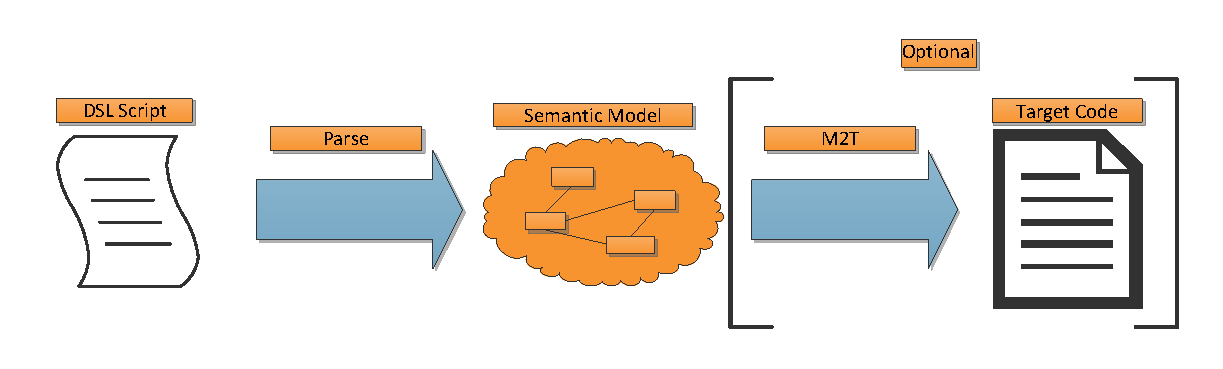
\includegraphics[scale=0.65]{images/dslm2t.pdf}}
    \caption[Domain Specific Language concept]{Figure shows how a DSL works.}
    \label{fig:dslm2t}
\end{figure}
\newpage
Figure \ref{fig:dslm2t} shows how a typical DSL works. Usually a DSL script is parsed and used to populate a semantic model which defines the semantics behind the script. As shown, model-to-text transformations are an optional part of DSLs. This is because DSLs are often used to allievate the configuration of a piece of software, and can be regarded as a thin wrapper around an API. Such DSLs are not necessarily focused on raising the level of abstraction, but rather to create a more convenient syntax for an API. In a MDE context, we want to raise the level of abstraction and provide the concrete semantics through model transformations.

Fowler~\cite{fowler2010domain} lists four main types of domain-specific languages:
\begin{description}
  \item[Internal DSLs] Internal DSLs are languages which are created within the host programming language. The host language is formed in a way that create a fluent syntax.
  \lstset{language=Java,caption=Simple internal DSL for creating specifications in DPF,label=list:internaldslexample,captionpos=b}
%   \begin{table}[ht]
%     \centering
  \begin{lstlisting}[showstringspaces=false]
builder
  .specification()
    .graph("m1")
      .node("DomainClass")
      .node("Type")
      .arrow("Attribute", "DomainClass", "Type")
      .arrow("Reference", "DomainClass", "DomainClass")
    .endgraph()

  .specification()
    .typeGraph("m1")
      .graph("instance")
	.node("Post", "DomainClass")
	.node("User", "DomainClass")
      .endgraph()
  \end{lstlisting}
%   \end{table}
  Listing \ref{list:internaldslexample} shows a simple internal DSL created in Java for populating a DPF model. This particular example uses \emph{method chaining}, a technique where a method (e.g. node()) returns its class instance when called.
  
  \item[External DSLs] External DSLs are the most common DSLs. These languages use external DSL scripts which are not bound be the host language's syntax and thus have a lot more syntactic freedom. Text files are parsed and used to either populate a semantic model, or do a model transformation (see figure \ref{fig:dslm2t}). Examples of such languages are SQL, HTML, XAML, Make etc.
 \lstset{caption=External DSL for creating specifications in DPF,label=list:externaldslexample,captionpos=b}
%   \begin{table}[ht]
%     \centering
    \begin{lstlisting}[showstringspaces=false]
mm:=TGraph<DPF>{
  z:Node-e0:Arrow->b:Node,
  a:Node-e1:Arrow->b:Node-e2:Arrow->c:Node-t:*->String,
}

m:=TGraph<mm>{
  b:c-y@1:t->["Hallo"],
  b:c-y@2:t->["Test"],
  f:a-l:e1->o:b,
}

ecore(mm)
    \end{lstlisting}
%   \end{table}
  Listing \ref{list:externaldslexample} shows an external DSL for defining \emph{DPF specifications}\footnote{The textual DPF tool is part of Florian Mantz' Ph.D. work.}. This example shows model \codeText{m} being typed by a metamodel \codeText{mm}, and then serializing the model. DPF is explained in section~\ref{sec:dpf}.
  \item[Fragmentary DSLs] These are DSLs which are embedded in the host programming language, such as \emph{regular expressions}.
  \item[Language workbenches] Discussed in section~\ref{sec:language_workbenches}.
\end{description}

\subsubsection{Domain-Specific Modelling Languages} 
DSMLs serve the same purpose as a DSL, but is usually presented in a visual manner. These languages are specified according to a \emph{metamodel}, sometimes defined as a "model of models"~\cite{rutle_thesis_2010}. The DSMLs are usually defined by domain experts and experienced developers to ensure that the domain concepts are properly described. The languages are then used by other developers as a programming tool. These languages are dependent on surrounding functionality and tooling, e.g. graphical editors, code generators and model validation. Workflow and tooling are further discussed in section~\ref{sec:language_workbenches}, Language Workbenches. 
\begin{figure}[htpb]
    \centering
    \centerline{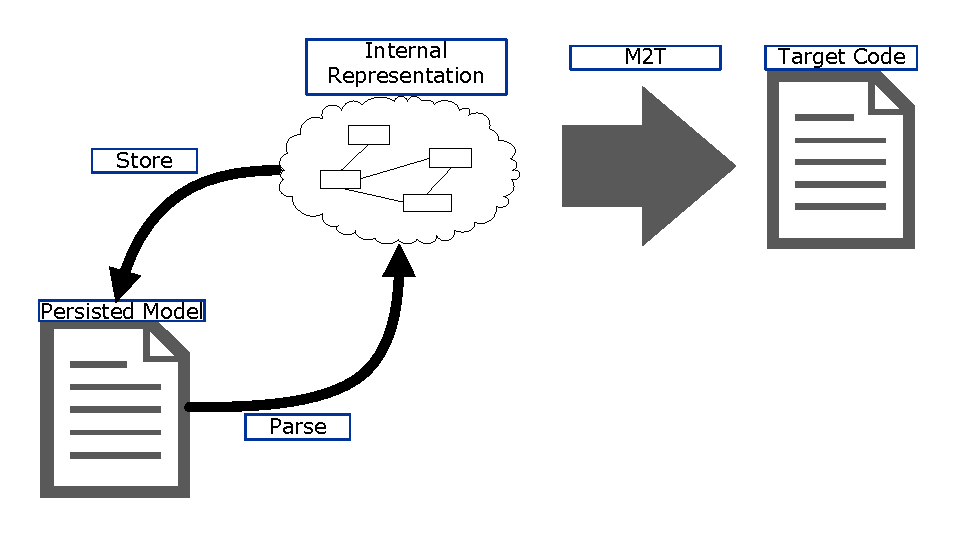
\includegraphics[scale=0.7]{images/dsml2.pdf}}
    \caption[Domain Specific Modelling Language tool]{An abstract view of a Domain Specific Modelling Language tool.}
    \label{fig:dsml2}
\end{figure}

The main difference between DSLs and DSMLs are the inner workings of the modelling environment. Both DSLs and DSMLs needs a parser which can translate the source file to an internal representation. The DSL's parser usually produce an abstract syntax tree or it populates a semantic model. 

Figure \ref{fig:dsml2} shows how the equivalent of the DSL script is the internal representation in a DSML-tool. The internal representation of the model is the model; the persisted model are only a means for the computer to understand the model. The model-to-text transformation (M2T) is not marked as optional as in figure \ref{fig:dslm2t}, because DSMLs require some kind of model transformation to have any meaning to a computer. 

The DSML is dependent on tooling, e.g. a visual editor which has an internal representation of the model. Usually this model also has an external representation in the form of a file. A popular format for this is the XML Metadata Interchange (XMI), a XML-based format that is tailored for representing models. Furthermore DSMLs are purely a MDE concept, and are rarely used to populate semantic models.
Model transformations with DSLs and DSMLs are discussed further in chapter~\ref{chap:code_generation}.

% Ein figur som viser DSML(persistence) -> parsing -> inner representation/semantic model -> m2t/m2m
% Ta med noko om korleis ein DSML er representert innad i verktøy

%that DSLs are constrained by a grammar that defines the language. This grammar is centered around the key concepts of a domain. 
% A DSML uses a base language in which you specify your metamodel(s) that in its turn defines the key concepts in the domain. 

% - dslar mot dsml \newline MOAR?

\subsection{Model-driven Architecture}
Model-driven Architechture is the Object Management Group's (OMG)~\cite{MDA} model-driven development initiative and can be regarded as a predecessor to MDE. It was launched as a standard in 2001. Even though the concepts of domain-specific modelling was known, OMGs MDA created new interest in the subject. Its core principle is to abstract away technology details of a specified system with the use of platform-independent models (PIM). PIMs contain business functionality and behaviour, and are reusable across any operating system/architecture. Before generating any code from a MDA project to a target environment, a platform-specific model (PSM) is created through \emph{model-to-model transformations}. A PSM is generated for each target environment. 
\begin{quote}
``The primary goals of MDA is portability, interopability and reusability through architectural separation of concern.~\cite{MDA}''
\end{quote}
MDA meets a lot of critique for different reasons. MDA uses model-to-model transformations to generate more detailed models as you go, i.e. from a PIM to a PSM resulting in the need to maintain more models than necessary. Another problem arise when you edit the PSM; how is this reflected in the PIM?

The MDA spec is centered around OMG's own standards. The modelling language used is very often UML, but it can be any \emph{Meta-Object Facility (MOF)} compliant modelling language. MOF is a closed metamodel hierarchy with four levels (see more in next section).

\section{Metamodelling}
Metamodelling is an important concept in MDE, yet its definition is highly debated~\cite{rutle_thesis_2010}~\cite{rossini_thesis_2011}. A metamodel is sometimes referred to as a "model of models"; Cook and Kent~\cite{cook:domainspecificide} claims this is a bad definition and should rather be ``a model of the concepts expressed by a modelling language''. A suitable definition could also be ``a model of a modelling language''. 

\begin{figure}[h]
    \centering
    \centerline{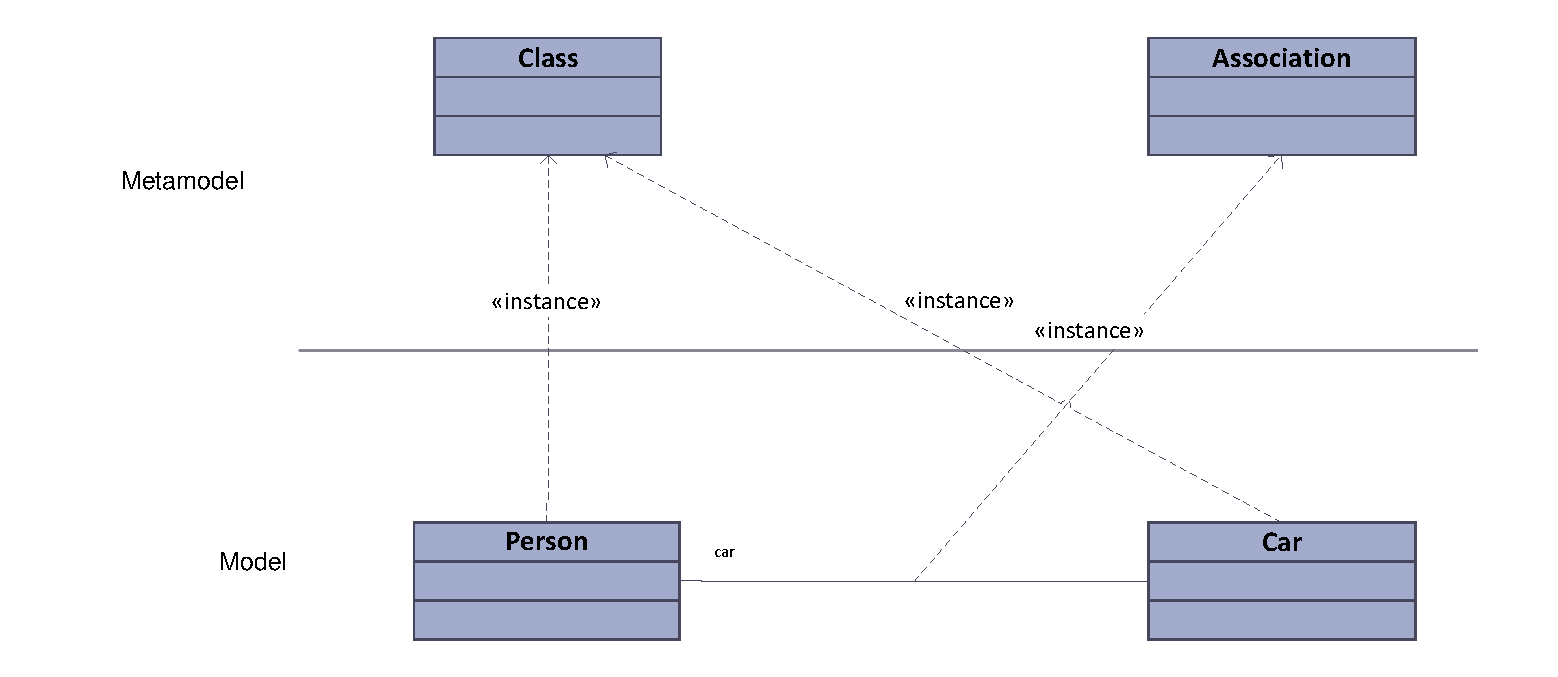
\includegraphics[scale=0.6]{images/uml_metamodel_example.pdf}}
    \caption[UML metamodel example]{A simple metamodel/model example.}
    \label{fig:uml_metamodel_example}
\end{figure}

Figure \ref{fig:uml_metamodel_example} shows a simple metamodelling example where each of the modelling constructs is an instance of a concept from the metalevel. A metamodel specifies the abstract syntax of a modelling language. This syntax defines the concepts, attributes, their relationships and how they fit together to create a valid model~\cite{rutle_thesis_2010}. A model's available features is defined by what features its metamodel defines. Metamodels has their own \emph{meta-metamodel} which define the syntax they must adhere to as well. The metalayer on top of the hierarchy is usually defined by a \emph{reflexive} modelling language, a language which is defined in itself.

In 1997 OMG adopted MOF 1.1 as a standard, around the same time as UML 1.1 was adopted. The goal of MOF is to create a common way of describing model metadata (data about models). This is done through a number of specifications such as MOF Core, MOF IDL Mapping, MOF XMI Mapping, MOF Model to text (MOFM2T) among others.

\begin{figure}[htpb]
    \centering
    \centerline{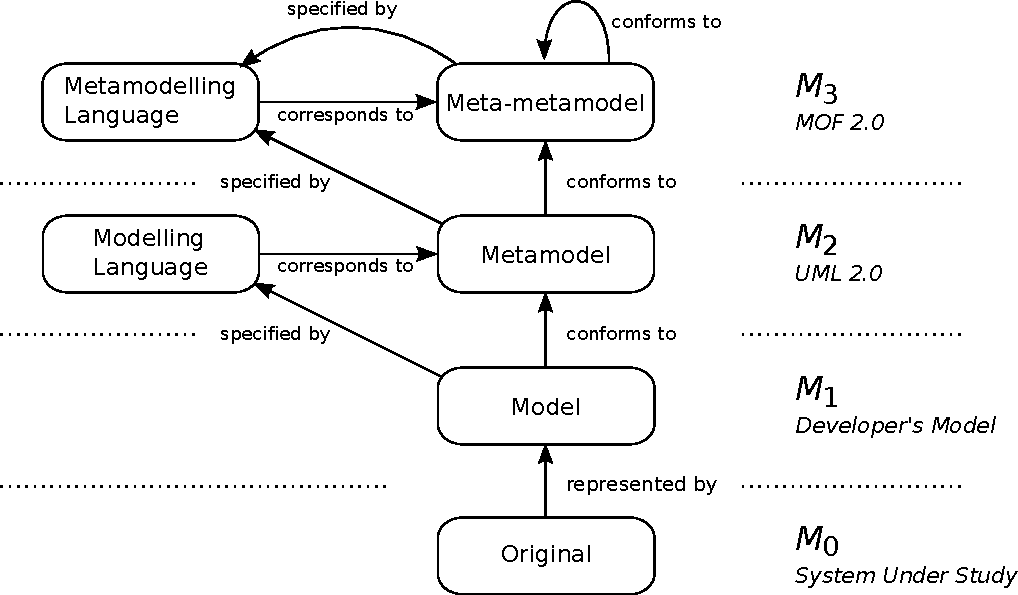
\includegraphics[scale=0.5]{images/omg_hierarchy.pdf}}
    \caption[MOF hierarchy]{Figure shows the four layer hierarchy defined in MOF.}
    \label{fig:mof}
\end{figure}

MOF defines a metamodel hierarchy with four layers (M$_{3}$ to M$_{0}$) where each level conforms to the level above it. MOF's goal is to create a "grammar" for how the models should be formed. MOF has two variants; Complete MOF (CMOF) and Essential MOF (EMOF). EMOF contains only the most basic constructs, which in broad strokes is classes, relations, types, packages and operations. Even though an EMOF compliant modelling language is enough for a lot of use cases, the language is fixed and thus falls short compared to the expressiveness of a DSML created without an EMOF compliant modelling language.

Figure \ref{fig:mof} shows that the M$_{3}$ level, the meta-metamodel, is defined in itself (\emph{reflexive layer}). This is done through constructs which the MOF specification provides. This layer is the metamodel for the UML language. The M$_{2}$ level is the instance of M$_{3}$, and is the model which implements UML, adhering to the abstract syntax of the layer above. The M$_{1}$ layer is where UML concepts such as Class, Atttribute and Operations are used to create a comprehensible model of the system which is then instantiated by level M$_{0}$, the \emph{system under study (SUS)}. M$_{0}$ contains the original, real world object, e.g. "Ford" would be instance of a M$_{1}$ class Car.

MOF is often under criticism in the literature for beeing, rigid because of a fixed number of metalevels (MOF is sometimes referred to as the four-layered hierarchy). This criticism is somewhat incorrect as the MOF specification does not restrict the number of layers~\cite{OMG07UML}. %7.12 i uml ref

% - Why several layers -> abstraction
% - fleirnivå grafisk modellering

\section{Constraints}
A constraint helps us to specify complex requirements beyond what basic modelling constructs can offer. In UML we have the option to apply constraints to our models. Unfortunately only simple constraints like multiplicity and uniqueness can be applied directly in the metamodel. These constraints are called \emph{structural constraints}. If we want to create a constraint which cannot be declared in the model, we need to create these externally. 

The "external" constraints are called \emph{attached constraints}, and are created using a declarative language like \emph{Object Constraint Language (OCL)}~\cite{OMG06OCL}. A solution like this is problematic; a UML model is a graph based model and OCL is textual language, making it harder to reason about the models. Not only for the developer, but also for the domain expert(s). There are also issues with reflecting changes in the model against the OCL constraints, creating synchronization issues~\cite{rutle_thesis_2010}. OCL is an OMG standard and is the recommended attached constraints facility used in combination with UML and MDA. 

\section{Language Workbenches}\label{sec:language_workbenches}
Language workbench is a term coined by Martin Fowler~\cite{fowler2010domain} that describes an environment for creating DSML/DSLs and corresponding tools. The workbenches should provide an IDE-like environment for creating DSML/DSLs, and in addition to generate code it should generate tooling for the specified language. Language workbenches are a relatively new concept which has been increasingly popular the last few years, and is under heavy research and changes. 
When working with language workbenches, the development process are divided into two phases. Figure~\ref{fig:lwusecase} shows how the DSML is created along with relevant tooling, such as editors and code generators. This activity should be performed by domain experts, as well as developers with experience. Using experienced developers will ensure that the tooling for the language is tailored to the users (which are developers). The figure also illustrates that developers utilize the domain-specific environment created from the DSML. \newline
\begin{figure}[hp]
    \centering
    \centerline{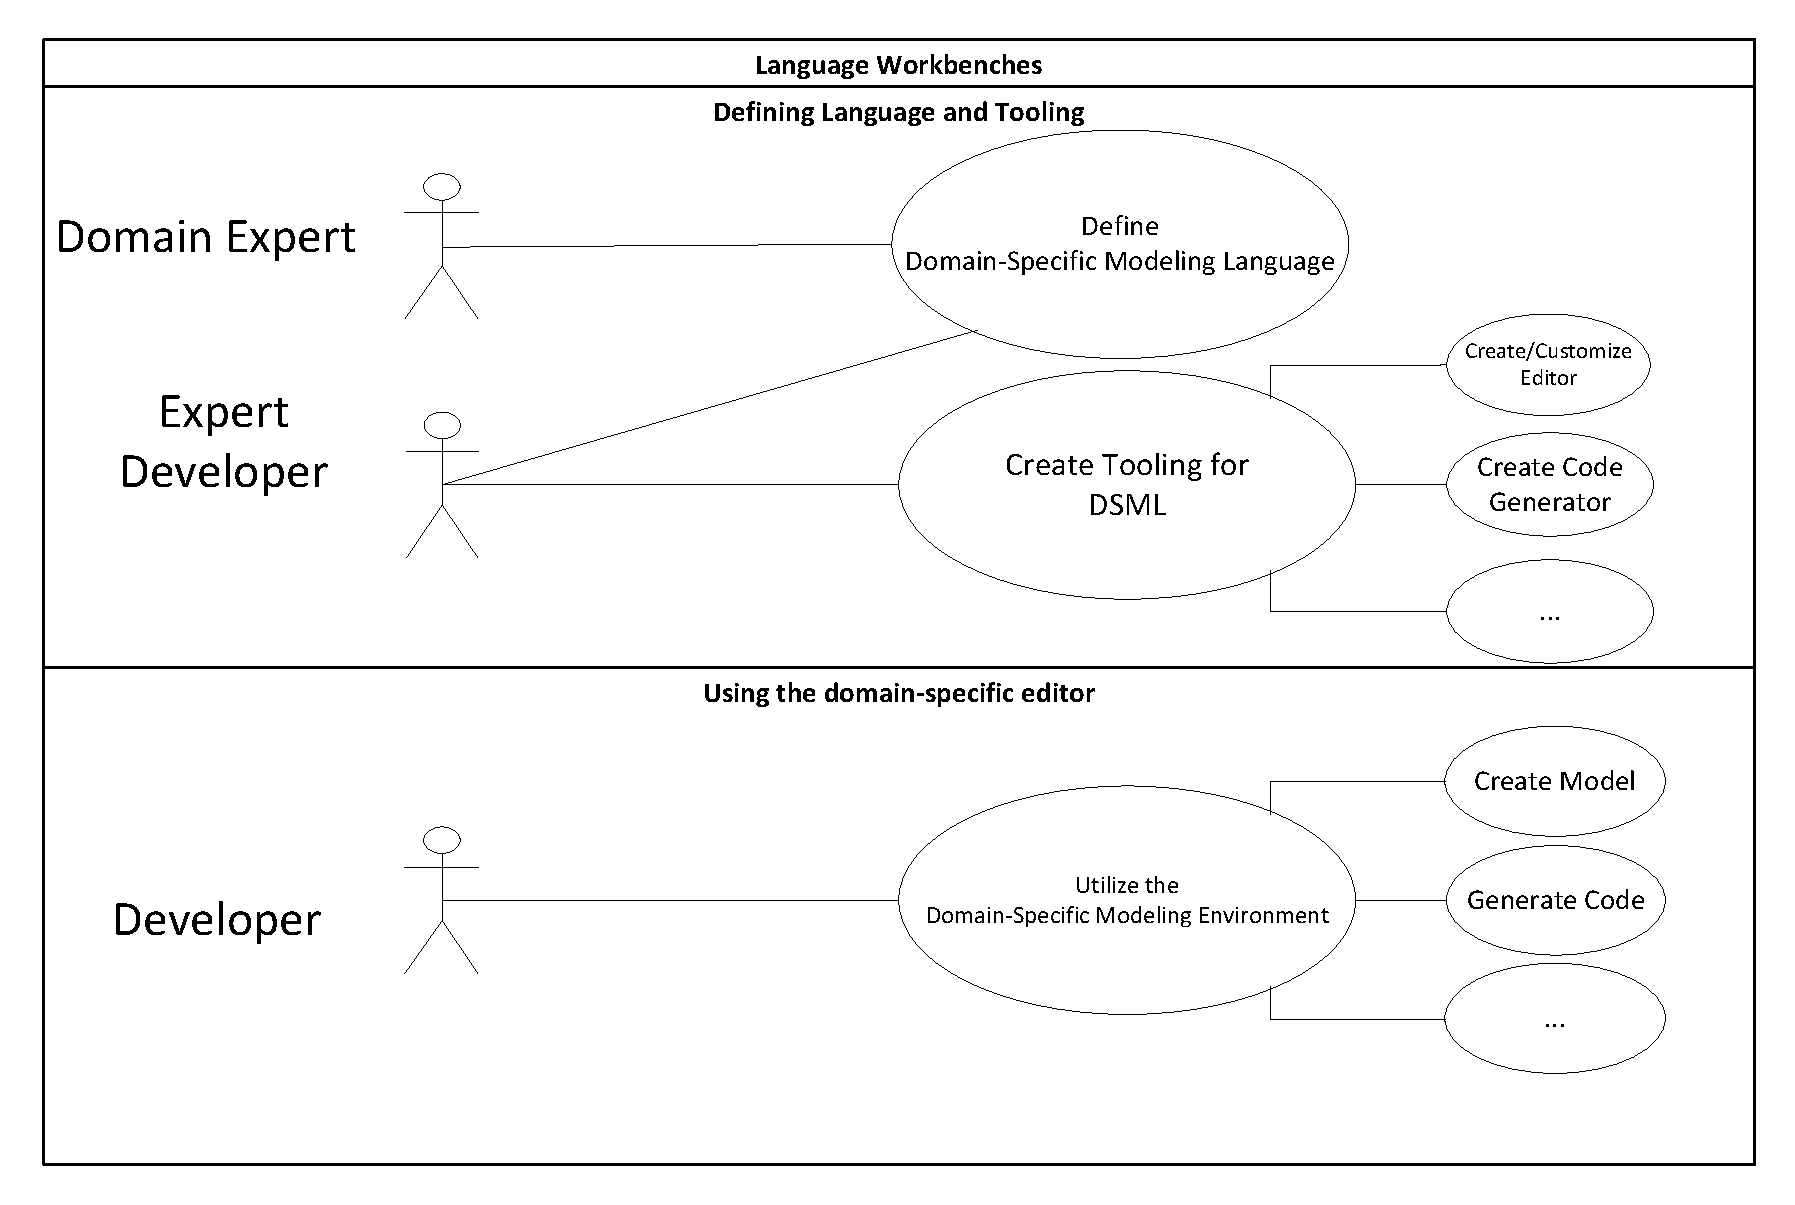
\includegraphics[scale=0.5]{images/LanguageWorkbenchUseCase.pdf}}
    \caption[Language workbench workflow]{Figure shows the intended workflow for a language workbench.}
    \label{fig:lwusecase}
\end{figure}

Martin Fowler describes a few common elements in a language workbench~\cite{fowler2010domain}:
\begin{description}
  \item[\emph{Semantic Model} schema] defines the structure of the \emph{Semantic Model}, based on a metamodel. In language workbenches the semantic model is the metamodel used for the model. Fowler uses the term \emph{schema} for the metamodel, or DSML if you like. The base model of the tool is called a \emph{schema definition language}.\newpage
  \item[DSML editing environment] defines an IDE-like experience when editing a DSML/DSL, often through \emph{projectional editing}.
  Projectional editing provides some kind of interface where we edit our models. Besides the diagrammatic approach, there are also schemas, forms, hierarchies etc. The counterpart of projectional editing is source editing, which is traditional programming using text files. Some language workbench solutions gives the opportunity of using multiple projections for your model, i.e. you can get a schema representation of a diagram based model, or a text representation.
  \item[Semantic Model behaviour] defines the semantics of the language specified. Usually this is achieved through code generation.
  Although the model is stored in the language workbench, the computer does not understand the intent of the model initially. The semantics of a DSML is defined through model transformations. The model can configure an API, create an interpreter, do a model-to-model transformation, but most often generating executable code (model-to-text transformation) is the chosen solution.
\end{description}

\begin{figure}[htpb]
    \centering
    \centerline{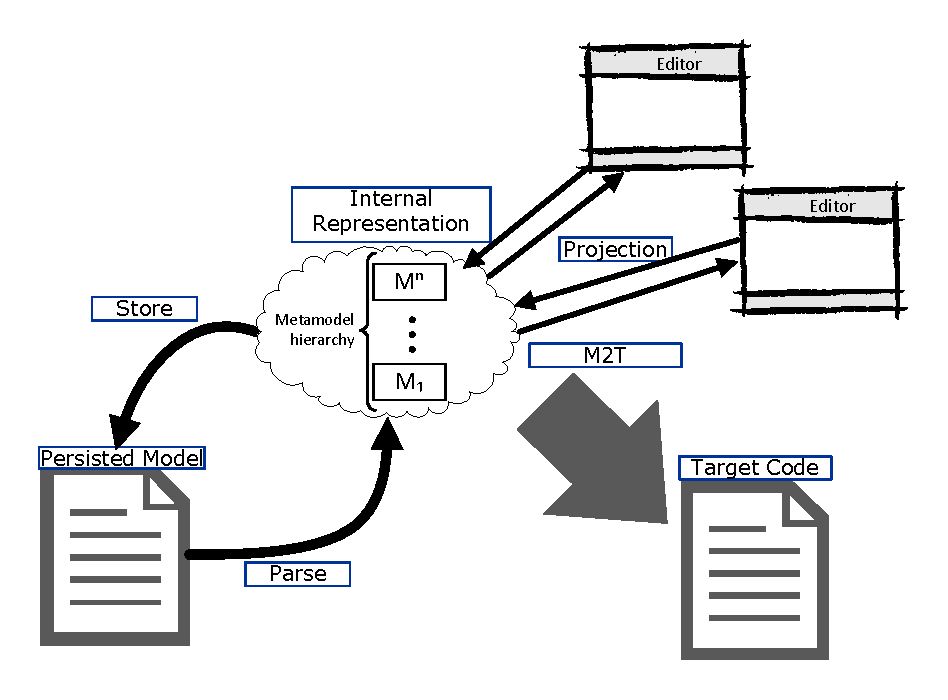
\includegraphics[scale=0.8]{images/dsml3.pdf}}
    \caption[Language workbench]{Figure shows a conceptual view of a language workbench.}
    \label{fig:dsml}
\end{figure}

Figure \ref{fig:dsml} shows how a language workbench work conceptually. At the heart of the language workbench, we find an internal representation of any models we operate on. This might be a single model, or a complete metamodel hierarchy. It forms the basis for the tools built around it. The tooling in a language workbench is defined as anything from the concept of a schema-definition language to code generators and constraint validation. The figure shows the most basic parts needed for a functional language workbench. As discussed in section~\ref{subsec:dsml} the internal representation of the model is the model. A persistence facility is needed for reuse and storing of the models. The persisted version of the models are not meant for hand editing, this should be done through the editing environment. 

% Rich tooling can enhance the modeling experience, but.

% In contrast to figure \ref{dslm2t} we see some differences; the equivalent of the DSL script is the internal representation of a DSML where persistence of the model is only used because we want the model to exist beyond the memory of a computer. The model is often stored in XMI, and is not made for handediting.
% MODELL SOM VISER KORLEIS SCHEMA LANG-> METAMODELL ->MODELL
% Figure [lol] shows 
% Along with tools like Obeo Designer and MetaEdit+, we find that DPF Editor fits these critera and introduces a new approach to domain-specific modeling. //MEH\newline
% define tooling\newline
% - Components: Model, generator, model framework/semantic model, target environment, dsm tooling, schema-definition language,\newline

\section{Existing Language Workbench Solutions} 
This section gives a brief overview of some of the more popular projection based language workbench solutions on the market today. 
% We will present some of the features of each solution.

\subsection{Eclipse and Eclipse Modeling Framework}
The Eclipse Foundation~\cite{Eclipse} is a non-profit organization which was established in 2004 with the goal of creating a vendor-neutral, transparent and open community around the Eclipse projects. The Eclipse eco-system consists of a vast amount of projects, everything from development tooling to SOA and web related projects. A common misconception is that when people think of Eclipse, they have Eclipse Java Development Tools (JDT) in mind. Eclipse JDT is a combination of different Eclipse projects, and provides a feature rich Integrated Development Environment for the Java programming language. This means Eclipse JDT is a collection of (in)dependent plug-ins which ultimately results in the IDE. The philosophy behind Eclipse is modularity; at the heart of Eclipse lies Equinox, an implementation of the OSGi core framework specification, which facilitates the modular nature of the \emph{Eclipse Platform}~\cite{eclipse_whitepaper}. All functionality in Eclipse is provided through plug-ins.

\subsubsection{EMF} \label{subsub:emf}
EMF (or rather EMF Core) is the project at the center of Eclipse's modelling technologies. The framework aims to unite Java, XML and UML; models in EMF can be expressed either way, where one can generate one representation from the other~\cite{BudinskyMerksS06}. EMF is a modelling tool which can be found in the middle of a pure modelling tool and Java code. Instead of following the "raising abstraction" mantra of pure modelling tools, EMF recognizes the need for a tool where the programmer can easily understand the mapping between model and code. EMF provides a modelling environment based on its own metamodel Ecore (which is a reflexive model). Ecore contains a basic set of modelling constructs that corresponds to EMOF. EMF also provide persistence and a code generation facility that can generate Java code from your metamodel, unit-tests for said code, and the possiblity to generate a simple hierarchy based editor. EMF does not facilitate code generation from the model instance level. This is handled by other modelling components, such as tools from the M2T (model-to-text) project.

\begin{figure}[htpb]
    \centering
    \centerline{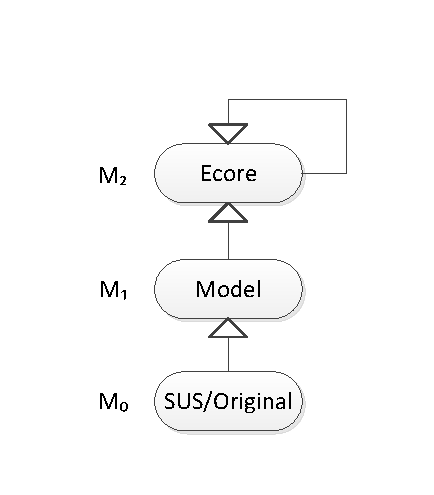
\includegraphics[scale=0.8]{images/ecoremof.pdf}}
    \caption[Ecore and MOF]{Figure shows a how Ecore fit into the MOF hierarchy.}
    \label{fig:ecoremof}
\end{figure}
Figure~\ref{fig:ecoremof} shows how Ecore fit into the MOF hierarchy. As the figure shows, EMF does not give you the possiblity of multiple metalevels. Although this restriction strengthens the intent of a comprehensible mapping between model and code, it makes it hard to create a DSML that can be substituted for code. An important note about Ecore's MOF hierarchy is that the levels vary based on what you try to achieve. With the use of the UML2 support, one have four levels as usual, but if you use Ecore to model a system directly, you only have three levels.

\begin{figure}[htpb]
    \centering
    \centerline{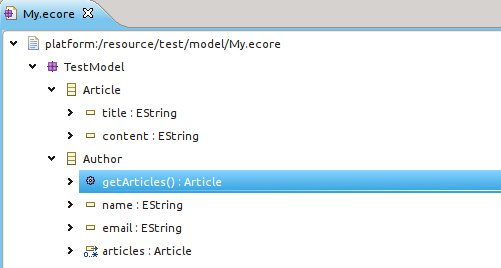
\includegraphics[scale=0.8]{images/emf_hierarchy.jpeg}}
    \caption[Creating an Ecore file]{Figure shows editing an Ecore file using the hierarchy view.}
    \label{fig:emf_hierarchy}
\end{figure}

\begin{figure}[htpb]
    \centering
    \centerline{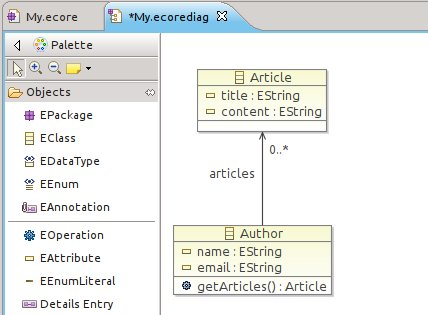
\includegraphics[scale=0.8]{images/emf_diagram.jpeg}}
    \caption[Creating an Ecore file diagramatically]{Figure shows editing an Ecore file using the graph based view.}
    \label{fig:emf_diagram}
\end{figure}

Figure \ref{fig:emf_hierarchy} and \ref{fig:emf_diagram} shows how the creation of a metamodel in Ecore. You can choose between the hierarchy solution, or a projectional view which requires the generation of an Ecore Diagram file.

EMOF defines a limited amount of modelling constructs, among them classes, attributes, references, packages and operations. These concepts are easy to understand for any programmer with a background in object oriented languages, and thus creating a clear understanding of the mapping between model and code. As the MOF standard~\cite{OMG06MOF} defines, constraints beyond cardinality and uniqueness are defined externally. In EMF one can define \emph{invariants} which are defined as a boolean method in the model, or a constraint which is defined as a method on a validator class, not in the model itself. Either way, hand editing is required to define what the constraint/invariant actually constrains. The implementations can use OCL if desired.

\subsection{Obeo Designer}
Obeo Designer is the product of a french company named Obeo. Obeo is a consulting company which has a strong focus on MDE and MDA. The company is an Eclipse Foundation Strategic Member and a contributor on many Eclipse Modelling projects. Obeo Designer is based on Eclipse EMF, which means it uses \emph{Ecore} as its modelling language. The tool's main focus is on creating visualizations for your model, as well as generators. 

\begin{figure}[hp]
  \centering
  \centerline{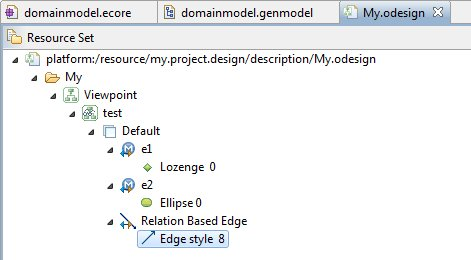
\includegraphics[scale=0.8]{images/obeo_graph_example.jpeg}}
  \caption[Creating graphs in Obeo Designer]{Example of creating a custom visualization for an Ecore model in Obeo Designer.}
  \label{fig:obeo_graphvisual}
\end{figure}

\begin{figure}[hp]
  \centering
  \centerline{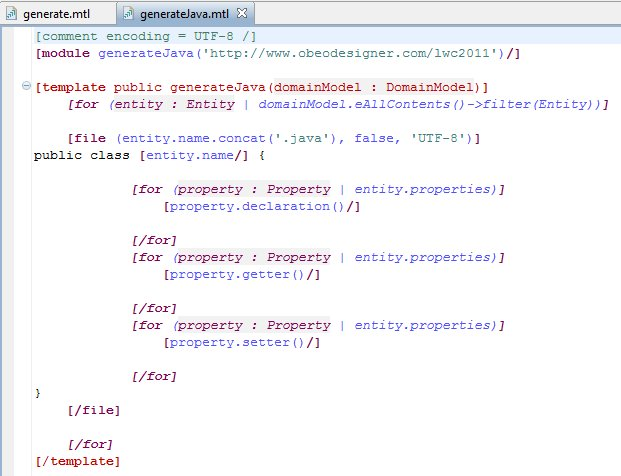
\includegraphics[scale=0.7]{images/obeo_generate_code.jpeg}}
  \caption[Creating templates using Acceleo]{Creating Acceleo templates for code generation.}
  \label{fig:obeo_code}
\end{figure}

Figure \ref{fig:obeo_graphvisual} shows the editor for creating custom visualizations for your Ecore model. There is no graphical editor for creating graphics, one have to choose from a set of pre-defined ones or use an external image. 

\newpage

One of the promoted features of Obeo Designer is the option of creating layers in your graph visualizations. This means you can create visualizations which fulfill a certain criteria. Take a family tree (a simple hierarchy) DSML as example; if we detect that two people are cousins, we can create a visualization that shows this by placing an arrow between them or similar.
% [set inn bilete med og utan layer] ?

Figure ~\ref{fig:obeo_code} shows Obeo's own code generation facility Acceleo~\cite{acceleo}. Acceleo is further reviewed in section~\ref{subsec:acceleo}.

Obeo Designer is split up in three products, based on what you need:
\begin{description}
  \item[Architect Edition] Full set of features. Suitable for creating editors and generators.
  \item[Developer Edition] Not possible to create editors. Intended for code generation template developers.
  \item[Standard Edition] Not possible to create either editor nor templates. This is edition is intended for \emph{using} the editors and generators.
\end{description}
% 
% -define visualisations and palettes based on ecore metamodel\newline
% -different visualisations (graph, table,tree,) \newline
% -code generation with acceleo\newline
% -different editions\newline
% -layers in the visualisation
% \newpage
\subsection{MetaCase MetaEdit+}
MetaCase's MetaEdit+~\cite{metacase} products are one of the most mature solutions on the market today. The company started out in 1991, having its roots in work from the University of Jyväskylä in Finland. The schema-definition language is based on the \emph{Object-Property-Role-Relationship (OPRR)} model. A MetaEdit+ metamodel consists of three parts; a GOPRR model, a code generator (specified with a custom DSL), and a graphical notation for the OPRR model. MetaEdit+ is split up in two different products, MetaEdit+ Workbench and MetaEdit+ Modeler. The workbench is used by the "metamodeler" to create a language, generator and graphical notation. The MetaEdit+ Modeler is used by developers to utilize the languages created in the Workbench, or with a pre-defined metamodel as basis. This follows the workflow shown in figure \ref{fig:lwusecase}.

\begin{figure}[hp]
  \centering
  \centerline{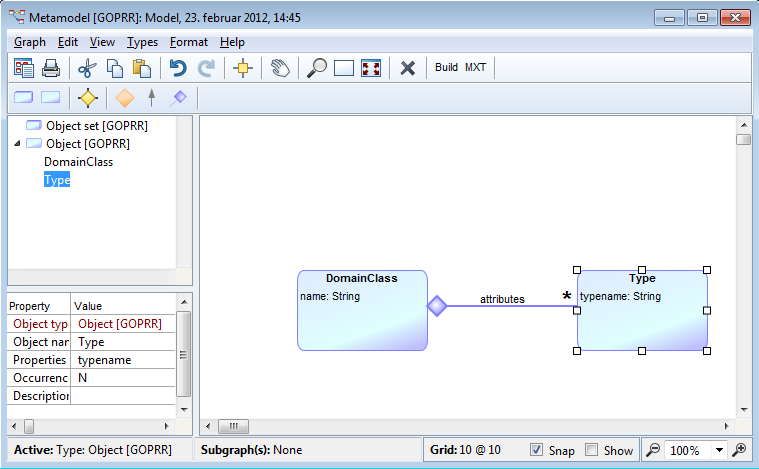
\includegraphics[scale=0.8]{images/me_mm_editor.png}}
  \caption[MetaEdit+ metamodel editor]{Figure shows the editor for metamodelling.}
  \label{fig:metacase_metamodel}
\end{figure}

Figure \ref{fig:metacase_metamodel} shows the editor where metamodels are created using \emph{GOPRR} which consists of the following modelling concepts~\cite{oprrmanual}:
\begin{description}
  \item[Graph] Specifies a modelling language.
  \item[Objects] This is the main type which is the node in the graphs. Used to model e.g. classes and states.
  \item[Object set] A collection of objects.
  \item[Property] This defines a property on a object. E.g name and ID.
  \item[Relationship] Connection between two or more objects. The relationships are connected to objects with roles. This is equivalent to an association in UML. 
  \item[Role] A role defines how an object behaves in a relationship. Each object in the relationship has a defined role. E.g. in an inheritance relationship, you have two roles: ancestors and descendants.
\end {description} 
GOPRR follows the four level hierarchy the same way Ecore does. You may model your system directly and "skip" a level, or specify another language. MetaCase includes a lot of languages for some more or less popular domains for reference and use. Among them we find DSMLs for insurance, UML, state machines, family trees, home automation etc.

\begin{figure}[hp]
  \centering
  \centerline{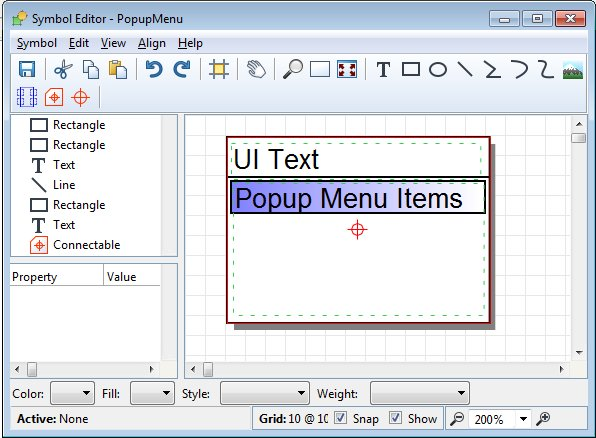
\includegraphics[scale=0.8]{images/me_symbol_editor.jpeg}}
  \caption[MetaEdit+ symbol editor]{Figure shows the editor for creating custom symbols.}
  \label{fig:metacase_symbol}
\end{figure}

One of the biggest features in MetaEdit+ is the ability to create custom symbols for the metamodel. These symbols can greatly improve the modelling experience for users of the DSML. Figure \ref{fig:metacase_symbol} shows the symbol editor where it is possible to draw a symbol or import graphics. This particular example shows a menu entry with a list of items in a Symbian Series 60 application DSML. The symbols can utilize particular aspects of the object entities.

\begin{figure}[hp]
  \centering
  \centerline{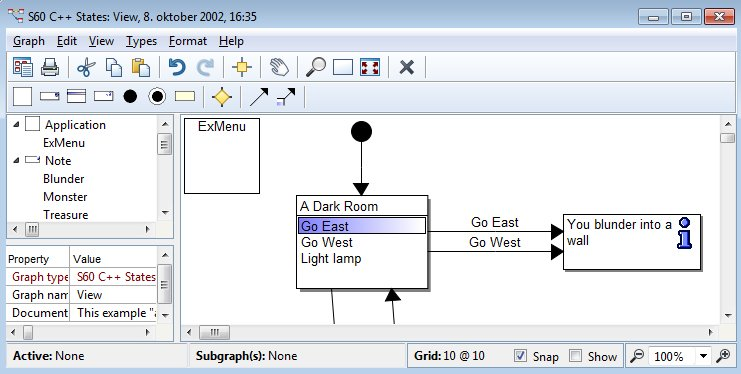
\includegraphics[scale=0.6]{images/me_instance_model_editor.jpeg}}
  \caption[MetaEdit+ instance model editor]{Editing an instance model of the Series 60 language in MetaEdit+.}
  \label{fig:metacase_metamodel}
\end{figure}

Figure~\ref{fig:metacase_metamodel} shows the creation of a Series 60 mobile application using the DSML defined in MetaEdit+. 

\begin{figure}[hp]
  \centering
  \centerline{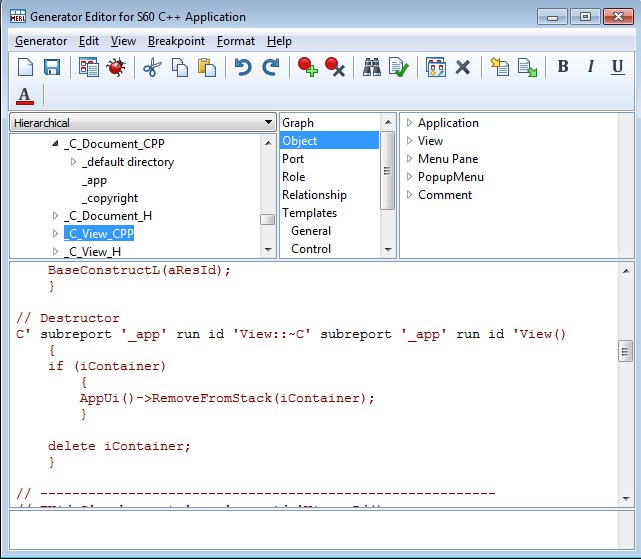
\includegraphics[scale=0.6]{images/me_template_editor.jpeg}}
  \caption[MetaEdit+ template editor]{Template editing in MetaEdit+.}
  \label{fig:metacase_template}
\end{figure}

Figure \ref{fig:metacase_template} shows the code generation template editor for the Series 60 example in \ref{fig:metacase_metamodel}. A metamodel can have several code generators associated with it.

Constraints in MetaEdit+ are created inside the model, which means that there is no support for \emph{attached constraints} (e.g. OCL). Unfortunately all constraints are pre-defined and there is no possiblity of creating custom constraints with corresponding symbol. All constraints are validated when modelling. A few of the pre-defined constraints include:
\begin{description}
  \item[Multiplicity]
  \item[Uniqueness]
  \item[Connectivity Constraints]
  \item[Explosions and Decomposition] \hfill \\
  A state in state diagram may be expanded into a separate diagram.
\end{description} 

The MetaEdit+ products are stand-alone proprietary software and is not built on Eclipse or similar platforms. It does however provide plug-ins for both Visual Studio and Eclipse with its new 5.0 release. MetaEdit+ supports Windows, Linux and Mac, but the latest beta release (which the illustrations are from) only supports Windows.

\section{Diagram Predicate Framework}\label{sec:dpf}
Diagram Predicate Framework (DPF) is an ongoing project at Bergen University College and the University of Bergen. The project started in 2006 with the aim to create a formal approach to MDE, with features as metamodelling, model transformations and model management. The framework is based on the Generalised Sketches formalism by Zinovy Diskin~\cite{DiskinKadish03}, and relies heavliy on mathematical concepts like category theory and graph transformations.

DPF facilitates a completely diagrammatic approach to MDE. DPF provides a multi-layer diagrammatic metamodelling hierarchy, where the need for attached constraints are removed. One of DPF's strengths is its general nature; it can be used as pattern to model other modelling language like UML, petri-nets and ER diagrams~\cite{RutleWolterL08TR367UIB}.

\begin{itemize}
  \item A DPF model consists of a \emph{specification $\spec{S}$} which consists of an underlying graph $S$, along with a set $\aconst{S}$ of \emph{atomic constraints $(\pi, \delta)$}.
%   \item A constraint $\pi \in \pred{\Sigma}$
  \item A signature $\sig{\Sigma} = \sigf{\Sigma}$ consists of a collection of predicate symbols $\pred{\Sigma}$.
  \item The constraints are instances of predicates $\pred{\Sigma}$.
\end{itemize}

A \emph{predicate} consists of a symbol, shape graph, visualization and a semantic interpretation. Predicates are defined within a \emph{signature}. Listing~\ref{list:multconstraint} shows the XML based definition of a multiplicity predicate. It defines a shape graph with two nodes and an arrow, a textual symbol \codeText{[mult(m,n)]}, and the semantic interpretation which is a Java based validator.

\lstset{language=xml,caption=A predicate for a multiplicity constraint.,label=list:multconstraint,captionpos=b}
\begin{table}[ht]
  \centering
  \begin{lstlisting}[showstringspaces=false]
<predicates symbol="[mult(m,n)]">
  <shape id="41921737-3a3a-4404-8d2a-a4ffe39da992" name="Default name">
    <nodes id="0867fde8-4eb6-4d42-be2d-715540a584d6" name="n_1"/>
    <nodes id="c4cce51b-3ab0-4e96-970a-18849131cbb3" name="n_2"/>
    <arrows id="554183df-2788-4469-ba63-84973bbb1d17" 
	target="//@predicates.10/@shape/@nodes.1" 
	source="//@predicates.10/@shape/@nodes.0" name="a_1"/>
  </shape>
  <semanticsValidator xsi:type="no.hib.dpf.core:MultiplicitySemantics"/>
</predicates>
  \end{lstlisting}
\end{table}

A central concept in DPF is graphs and graph homomorphisms. A graph homomorphism $\varphi$ is a mapping from a graph $G$ to another graph $H$, where the mapping preserves the source and target of each arrow. An atomic constraint $(\pi, \delta)$ in DPF consists of a predicate symbol as well as a graph homomorphism which defines what parts of the graph it constrains.

DPF defines two types of conformance relations which is \emph{typed by} and \emph{conforms to}. A meta-level $\spec{S}[i]$ is typed by the meta-level above $\spec{S}[i+1]$ if there is a graph homomorphism (also called \emph{typing morphism}) between the two meta-levels' underlying graphs: $\iota[i] : S[i] \rightarrow S[i+1]$. A specification $\spec{S}[i]$ at metalevel $i$ is said to conform to a specification $\spec{S}[i+1]$ at metalevel $i + 1$ if there exists a typing morphism $\iota[i] : S[i] \rightarrow S[i+1]$ such that $(S[i], \iota[i] )$ is a valid instance of $\spec{S}[i+1]$ ; i.e.  $\iota[i]$ satisfies the atomic constraints $\aconst{S}[i+1]$~\cite{dpf_editor_article}~\cite{rutle_thesis_2010}. See ~\cite{rutle_thesis_2010}~\cite{rossini_thesis_2011} for further discussions on DPF.

% A graph homomorphism consists of a pair of maps from the nodes and arrows of a graph to those of another graph, where the maps preserve the source and target of each arrow.
%  A specification Si at metalevel i is said to conform to a specification Si+1 at metalevel i + 1 if there exists a typing morphism ιi : Si → Si+1 such that (Si, ιi ) is a valid instance of Si+1 ; i.e.such that ιi satisfies the atomic constraints C Si+1 

% n DPF, two kinds of conformance relations are distinguished: typed by and conforms to. A spe-cification Si at metalevel i is said to be typed by aspecificationSi+1 at metalevel i + 1 if there exists a graph homomorphism ιi : Si → Si+1 , called the typing morphism, between the underlying graphs of the specifications. 
% - models are represented by diagrammatic specifications
% - specifications consists of a graph and a set of atomic constraints
% - Constraints are specifified in a predicates
% - predicates are defined in a signature
% - each predicate has an arity, a visualisation and a semantic interpretation
% - a dsl is a diagrammatic editor which consists of a signature and a metamodel
% -constraints and ocl\newline
% -grafhomomorfismar -> direkte typing frå ein node til ein anna node elns

\section{DPF Editor}

The DPF Editor is the reference implementation of DPF and its concepts~\cite{DPF_web}. There have been a few attempts the last years to implement earlier versions of DPF. The first attempt was performed by Ørjan Hatland in 2006~\cite{Hatland06}, a tool based on Microsoft .NET technology. This implementation was never completed and was not considered to be a good foundation for further development. In 2008, Stian Skjerveggen began the work on an Eclipse based solution~\cite{Skjerveggen08}. The core technology in this project was Graphical Modelling Framework (GMF)~\cite{GMP}, a framework that facilitates generation of graphical editors and tooling, based on EMF and Graphical Editing Framework (GEF). GEF facilitates creating rich graphical editors in Eclipse. This technology is somewhat "low-level", and requires a bit of work to achieve the same level of functionality which GMF can generate. GMF was at the end of the project deemed unsuitable for an implementation of DPF.

In 2010, Øyvind Bech and Dag Viggo Lokøen started the work on the current implementation of DPF, the DPF Editor~\cite{Bech11}. It is written from scratch using EMF and GEF and supports the most essential features concerning metamodelling:

\begin{itemize}
  \item Graph based projectional editing of models
  \item Storing/loading the models as XMI
  \item Arbitrary number of metalevels
  \item Checks typing between metalevels if there exists a graph homomorphism
  \item Checks constraints between metalevels
  \item Creation of predicates and corresponding Java validators
  \item Different simple symbols on nodes (circle, ellipse, rectangle etc.)\footnote{The creation of predicates and visualizations are later work by Ph.D. student Xiaoliang Wang.}
\end{itemize}
% \footnotetext[2]{The creation of predicates and visualisations are later work by Ph.D. student Xiaoliang Wang.}

None of the previous attempts to create DPF based software has reached a level of maturity where facilitating code generation was considered. 

\begin{figure}[htpb]
  \centering
  \centerline{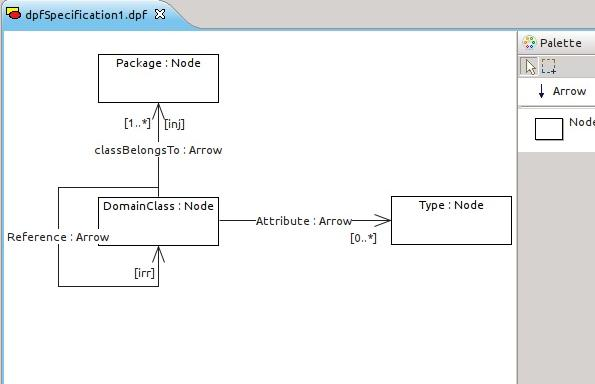
\includegraphics[scale=0.6]{images/dpf_editor.jpeg}}
  \caption[DPF Editor]{Creating a DSML in the DPF Editor.}
  \label{fig:dpf_editor}
\end{figure}

Figure~\ref{fig:dpf_editor} shows the editor view in the DPF Editor. We start off with only \codeText{Node} and \codeText{Arrow} when creating a DSML. The figure depicts a simple language for creating domain classes in web application. This model forms the basis for the tool demonstration i chapter~\ref{chap:case_study} and will then be explained further. Figure~\ref{fig:dpf_hierarchy} shows a subset of the DSML in figure~\ref{fig:dpf_editor} and how the different metalayers are typed by each other. The dotted lines shows conformance between the types levels.

\begin{figure}[htpb]
  \centering
  \centerline{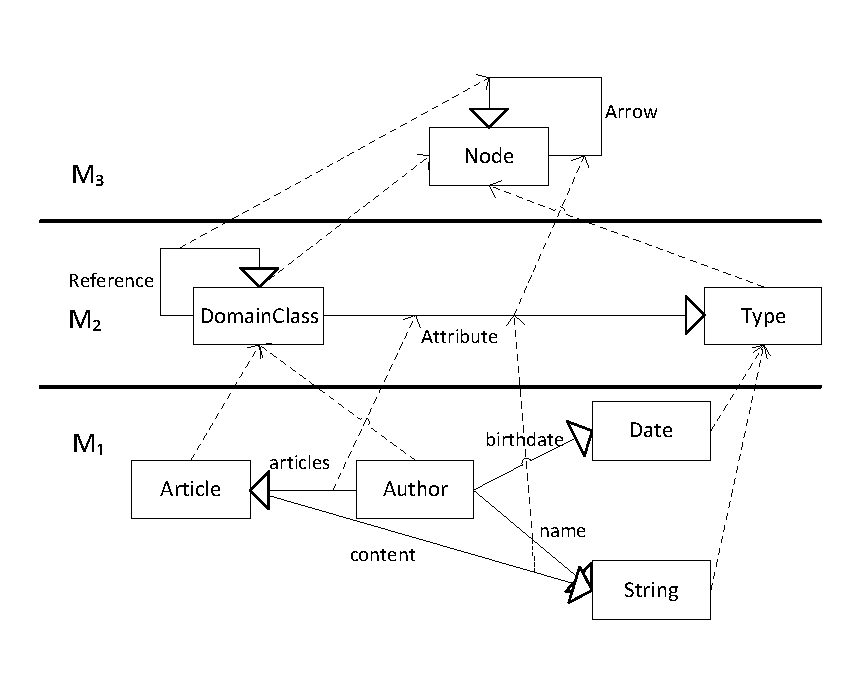
\includegraphics[scale=0.8]{images/dpf_hierarchy.pdf}}
  \caption[DPF DSML example]{Shows how the different DPF layers of a simple domain class DSML conforms to each other.}
  \label{fig:dpf_hierarchy}
\end{figure}

% The DPF Editor is under heavy development with the addition of new functionality all the time.
% [bilete av editor med model]
% [teikna eit hierarki elns]
% [bilete av predicat editor]
% [Klassediagram som viser dpf metamodell?]
% \begin{itemize}
%   \item Illustration showing the tool
%   \item Graphic editing of models
%   \item Metamodelling and typing of specifications
%   \item Constraints
% \end{itemize}
\newpage
\section{Comparison}
The evaluated tools has its strengths and weaknesses from a language workbench point of view. The concept of a language workbench is a pragmatic one, and this emphasizes usability of the tools. Even though EMF, Obeo Designer and MetaEdit+ are all mature products with a lot of users, they do not necessarily do everything right. A common problem is messy unintuitive user interfaces which significantly raises the bar for learning the software. 

The most complete (and most mature) tool, is MetaCase's MetaEdit+. It supports a wide variety of pre-defined popular modelling languages, but also has its own schema definition language, GOPRR. Obeo Designer improves on the shortcomings of plain EMF, with the possiblity of creating custom visualizations and support for code generation on the model level with Acceleo. Table~\ref{tab:lw_features} shows that a common trait between the three evaluated solutions; all support different forms of projections. The \emph{Projection Types} row use capital letters for describing a projection type:
D for diagrammatic, H for hierarchy, M for matrix and T for table.

Of the reviewed solutions we see that only the DPF Editor provides multi-level metamodelling, while the other adheres to the levels of MOF. As described, all three reviewed tools have a fixed number of metalevels. The metalevels may vary, because one can define e.g. UML through MOF's modelling facilities as shown in figure~\ref{fig:mof}. When it comes to constraints, we see that EMF only have support for \emph{structural constraints} inside the model and is dependent on external functionality for more advanced constraints. Since Obeo Designer is built around EMF, the same applies. MetaEdit+ has, like the DPF Editor, support for more advanced constraints within the model. There is however no option for defining constraints like in the DPF Editor, as they are fixed.

The DPF project can learn from other tools as there is a lot of room for improvement. The lessons learned are both good and bad; the tools studied all have usability issues, mostly related to complicated user interfaces. Having to use OCL for constraints also complicates the modelling process. Ideas like the symbol editor and multiple ways of projecting the model are some of the interesting features which the other tools more or less provide. 

A "projection" which none of the tools provide, are textual representation of the models (beyond serializing). The \emph{Language Workbench Competition (LWC)} which is a part of the \emph{Code Generation}~\cite{lwc} conference, refers to a language workbench that supports both diagrammatic and textual representation of a model as "the one language workbench to rule them all"\footnote{Florian Mantz has created a textual version of DPF in his Ph.D. thesis work. This work is currently not integrated with the DPF Editor.}. 

\let\Oldarraystretch\arraystretch
\renewcommand*\arraystretch{1.5}

\begin{table}[htb]  
  \flushleft
  \resizebox{1\textwidth}{!}{
    \begin{tabular}{|p{34mm}|p{26mm}|p{30mm}|p{22mm}|p{23mm}|}
      \hline
      \textbf{Tool}                   & \textbf{EMF}  & \textbf{Obeo Designer}  & \textbf{MetaCase MetaEdit+} & \textbf{DPF}\\
      \hline
      \textbf{Schema~Definition
	  \newline Language}          & Ecore                  & Ecore                             & GOPRR                    & DPF \\
      \hline
      \textbf{Symbol Editor}          & No                     & No                                & Yes                      & No \\
      \hline 
      \textbf{Projection
	\newline Types}               & D/H\footnotemark       & D/H/M/T                           & D/H/M/T                  & D \\
      \hline
      \textbf{Code~Generation
	\newline Facility}            & Yes\footnotemark       & Yes (Acceleo)                     & Yes                      & No \\
      \hline
      \textbf{Multi-level 
	\newline metamodelling}       & No                     & No                                & No                       & Yes \\
      \hline
      \textbf{Constraints}            & OCL                    & OCL                               & Model-based/Fixed        & Model-based/Custom \\
      \hline
      
    \end{tabular}
  }
%    \scalebox{0.77}{
%     \begin{tabular}{|p{26mm}|p{34mm}|p{25mm}|}
%       \hline
%       \textbf{Tool}                   & \textbf{Multi-level metamodelling}  & \textbf{Constraints}  \\
%       \hline
%       \textbf{EMF}                    & No                        & OCL                     \\
%       \hline 
%       \textbf{Obeo Designer}          & No                        & OCL                     \\
%       \hline 
%       \textbf{MetaCase MetaEdit+}     & No                        & Model-based/Fixed      \\
%       \hline
%       \textbf{DPF}                    & Yes                       & Model-based/Custom     \\
%       \hline
%     \end{tabular}
%   }
  \caption {Language workbench features}
  \label{tab:lw_features}
\end{table}
\footnotetext[4]{EMF provides a diagrammatic view for the metamodel, but not for the models.}
\footnotetext{EMF generates editors and code for your metamodel, but does not facilitate code generation from the instance model.}
% template language, profiler, template editor, custom generator metamodel, 
\let\arraystretch\Oldarraystretch




\chapter{Code Generation}\label{chap:code_generation}
This chapter will give an understanding of the concept code generation, as well as the motivation behind it. The section Framework Analysis (\ref{sec:framework_analysis}) will evaluate a few chosen code generation solutions, with a comparison at the end. Lastly, the Xpand code generation framework will be introduced. 

% Things to add:
% \begin{itemize}
%     \item Conceptual -> What is CG? figur som viser m2t?
%       \begin{itemize}
% 	\item Benefits (1.2 Herrington)
% 	\item efficiency (4.4.2 Tolvanen)
%       \end{itemize}
%     \item How to do CG
%     \item model transformations in DSLs and DSMLs
%     \begin{itemize}
%       \item Templated Generation - source listing/eksempel, figur som på wikip.
%       \item Transformer Generation - source listing/eksempel
%     \end{itemize}
%     \item what to generate -> everything? configuration code for a framework? Target framework?	
%     \item editing generated code -> gen code analogous to compiled c code
%     \item more about workflow?
%     \item samanlikningstabell på botn
%     \item rename chapters
% \end{itemize}
% Figur som viser den forskjellen mellom vanlig templateengine og den tolka approachen i Xpand. Må visa at templaten conforme til tolka typar istadenfor "ekte" typar
% Døme på figurar i herrington 2.2 og figur 12.1 i DSMbook
% Dropper diskusjon om kodegenering er beneficial, kostnad osv sidan CG er "oblig". Den diskusjonen høyrer til MDE
\section{What is Code Generation?}
Code generation, also called \emph{automatic programming}, is the process of automatically generate source code from some kind of specification (e.g. models). The user specifies \emph{what} to do, the computer generates source code which perform the task. Generating code is a common practice in todays software development, where modern IDEs in particular take advantage of this technique. The popularity of large middleware platforms, such as Java EE and Spring, has shown the advantages of code generation with its extensive need for configuration. These configuration files are often written in XML and are tedious and time consuming to write by hand. Another example is project wizards in IDEs which generate the needed configuration and templates for your project. The focus in this thesis will not be on generating specific configuration files for an arbitrary framework, instead we will focus on a general solution for creating production code from domain-specific models. These models can indeed result in build scripts or XML, however we want to generate production grade code for certain aspects of a system.

Generating code is done through a model transformation, more specifically model-to-text transformations. Through a set of transformation rules, we generate text which results in usable code. A transformation rule could be an expression in a template, or simply plain Java code that outputs a string based on some satisfied statement. In language workbenches code generation is very common, as the tool itself usually do not run the DSML which is created. DSLs on the other hand, is very often used as a wrapper around an API.

\section{Why use Code Generation?}
Using code generation yields a lot of advantages not only in the context of MDE, but also as a general technique in the programmers toolbelt. Herrington~\cite{herrington:codegeneration} lists a few: 
\begin{description}

\item[Consistency]
The generated code has a consistent feel, using the same naming conventions and style. This results in familiar interfaces for the users.

\item[Quality]
Having many programmers creating handwritten code may result in an inconsistent code base that must be updated manually on API changes. If this code can be generated, the generator has the advantage of generating all the classes at once which reflects the changes made.

\item[A single point of knowledge]
A change within e.g. a database, can have a chain reaction in your project; code, documentation and build scripts needs to be changed. This can be avoided using code generation.

\item[More time for development]
After spending the initial time-cost of creating proper models and generators, one can save a lot of development time. This is time that can be spent creating new features, and/or fixing existing ones.

\item[Abstraction]
The power of domain-specific modelling enables us to express more functionality in a consise manner.

\end{description}

Even though the benefits are big, there are always concerns about the code being generated, such as quality and efficiency. In the CASE-tools era, the fixed general modelling languages made it difficult to generate anything other than static code/schema definitions. With domain-specific modelling we are now able to generate both the static and functional code. This contrast may be the source to some of the skepticism we see today. The efficiency concern is about generating code for e.g. an embedded system with very limited resources, where handwritten code often is optimized with different workarounds and hacks. 

These concerns are as old as computing; when programming languages with a higher abstraction level came to existence, there was always concern that these languages could never generate code as good as hand written machinecode. History has shown that if given enough time, compilers become so advanced and effective that it is not feasible to hand write low level code for the sake of efficiency. Compilers do a lot of optimizing on its own, and any particular hacks used could easily be included in the generator, and thus creating as efficient code as the handwritten counterpart. The expressiveness of models gives us the power to create functional code which is safe and efficient; it really comes down to how the model and generator is defined. 

Tolvanen and Kelly~\cite{tolvanen:dsm} claims boldly:
\begin{quote}
``When code is produced by a generator made by an experienced developer, it will always produce better code than the average programmer writes manually.'' 
\end{quote}

\section{Creating a Code Generator}\label{sec:create_generator}
In a MDE environment, we need our models understood by a computer. The usual way of doing this is to either generate code, generate an interpreter or populate a semantic model. The last option is more likely to be used with textual DSLs rather than a DSML created in a language workbench, and is less relevant in the context of the \pluginName.
When creating a code generator, there are two things that is needed; the input (DSML) and a sample output of what you want to generate. After all, code generation is a model transformation. Through our generator, we express rules that maps our input to the output. If you attempt to create the generator first, you can end up creating a language that is to general for your domain. When you have both the output and the model in place, the generator creation will be a much simpler task. 

\begin{description}
  \item[Transformer Generation]
  This method uses a programmatic approach, where a generator traverses an input model directly in the programming language, and creates code statements. This approach is suitable when targeting one specific environment (although it can be generalized) and most of the code is generated from the model, i.e. low amount of static code.
\lstset{language=Java,caption=Example showing a Java method building code.,label=list:transformergeneration,captionpos=b}
% \begin{table}[ht]
%   \centering
\begin{lstlisting}[showstringspaces=false]
public String buildClass(Node n) {
    StringBuffer buf = new StringBuffer();
    
    buf.append("public class " + n.getName() + " {");
    
    for(Attribute a : n.getAttributes()) {
	buf.append("private " + a.getType() + " " + a.getName() ";");
    }
    
    buf.append("public " n.getName() + "{");
    buf.append("}");
    buf.append("}");
    
    return buf.toString();
}
\end{lstlisting}
% \end{table}
  Listing \ref{list:transformergeneration} shows a simple Java example where we build a class with private instance variables and a default constructor. Although easy to understand, these classes can grow very big when generating advanced functionality. Another issue is formatting the output; one needs to either format it as you create the code, or after. Formatting as you go, requires a way to keep track of indents and newlines. Formatting after the code is generated can be achieved by exploiting an existing formatter, like what Eclipse Java Development Tools provides, instead of creating one from scratch.
  \item[Templated Generation]
  Templated generation consists of a \emph{template engine}, a template language and sometimes a standard library that provides simple functionality for use within the templates. A template engine uses external files, called the templates, which uses a template language. This language uses markers to identify where certain parts of the code should be insterted. A template based solution is recommended when you have a lot of static code and/or configuration code, or you want to target several environments. This approach is the one chosen for this thesis and is investigated more in section \ref{sec:framework_analysis}.
\end{description}

Another issue that needs to be addressed is what you want to generate with your generator. Most of the time, there is no need to generate a complete runnable application. A common practice is to generate code for a \emph{domain framework} in your target environment. If no such framework exists, it might be a good idea to investigate the possibility of creating one. Such frameworks can greatly simplify the generated code by abstracting away repeated concepts.

\subsubsection{Model-to-model Transformations (M2M)}
Creating textual output from a generator is not always the best solution. Sometimes generating a new model might fit the development workflow better. A motivation for such a scenario is that the model is not descriptive enough to directly generate code. A real world example of this is the MDA workflow, where PIMs are transformed into PSMs as a step on the path to textual output.

\section{Editing Generated Code}
Ideally the generated code should work on its own, without any editing. This is a consequence of the effort put in when creating the DSML and associated tools. According to Kelly and Tolvanen~\cite{tolvanen:dsm}, a proper DSML should be analogous to compiling general programming language code.
The reality is somewhat different as the need for mixing generated and handwritten code is not seldom. The general rules are not to modify generated code and keeping generated code separated from handwritten code. To achieve these goals there are a few techniques~\cite{fowler2010domain}:
\begin{description}
  \item[Keep generated code in a separate folder] \hfill \\
  This reduces the risk of editing code and losing the changes upon regeneration.
  \item[Partial classes] \hfill \\
  Partial classes provides the option of splitting classes into separate files. This is supported by Smalltalk and C\#. This is however not supported in Java, C++ etc.
  \item[Generation gap pattern] \hfill \\
  Generation gap pattern is probably the most general solution for this problem. It uses inheritance to extend functionality; a generated class acts as a superclass which you inherit with a handwritten class. The only drawback is the need for relaxing visibility rules in the superclass.
  \item[Annotations] \hfill \\
  This approach lets you mix handwritten and generated code using annotations (Java) or attributes (C\#). In some cases this might be the best solution. E.g. when generating code from an EMF model, it is often necessary to hand code some of the functionality in declared operations. It is then possible to use annotations to mark which methods should be generated or not with the \codeText{@generated NOT} annotation.
  \item[Protected Regions] \hfill \\
  With protected regions you place a marker, often a start marker and an end marker, in the source code where you want the generator to not re-generate. This can be seen as a general approach to annotations based protection.
\end{description}

\section{Metamodels and Code Generation}\label{sec:metamodels_and_cg}
So far the discussion has revolved around general principles and techniques concerning code generation. When using template based solutions (see \ref{sec:framework_analysis}) one operate directly on objects in the host language. The template engines were probably not built with MDE in mind and are thus more general. One of the biggest uses are rendering web pages. In the context of models, one would work directly on the model's internal representation, like listing~\ref{list:smalljet} shows. 
\lstset{caption=Simplified Java Emitter Templates (JET) example of using an object directly.,label=list:smalljet,captionpos=b}
\begin{table}[ht]
  \centering
\begin{lstlisting}[showstringspaces=false]
<% Node n = (Node)argument;%>
class <%=n.getName()%> 
\end{lstlisting}
\end{table}
There is one big drawback of this approach, and when our solution is supposed to facilitate code generation for any arbitrary model, it is quite essential: there is no way of expressing domain concepts in a simple elegant manner. Giving the user a template engine and a clean template for their DSML would work, but do not address the problem at all. We need to express the most essential part of MDE, the \emph{domain concepts}, in such a way that it is intuitive and easy to create code generators.

To express the domain concepts we need to look at the DSML, not the model (instance). The goal is to express an arbitrary DSML and its concepts in a chosen template language. Creating such a solution from the beginning would entail a lot more work than the time-frame of this thesis would allow. Luckily, the Eclipse M2T project has addressed this issue with a few solutions described in the next section. 

% \begin{itemize}
%   \item Creating generator before model (results in general model)
%   \item Fear of creating model thats hard to map against code
%   \item Useful to have example input/output before creating generator
%   \item Generated code not always runnable on its own, often configuration code for domain framework or target environment
%   \item Generated code is analogues to compiled C.
%   \item Code example listings in both transformer generation and templated generation.
% \end{itemize}


\section{Framework Analysis}\label{sec:framework_analysis}
This section gives a brief overview of the different code generation solutions that was considered in this project. The chosen solution, Xpand, is introduced with a short overview of features. This will be discussed in detail in section \ref{sec:xpand}.

\subsection{Template Engines}
Both JET and Velocity are simple template engines, which provide nothing more than an engine, a template language and a “standard library” with functions to alleviate the use of Java code in the templates. Choosing these solutions would entail the creation of an API that exposed the desired functionality; the domain concepts of the DSML and associated operations/methods. Creating an API like this would be a messy complicated solution. 

Creating editor support which exposed the DSML properly would not be an easy task to achieve as these engines have no interpreter which could interpret the models during runtime.
\begin{figure}[pb]
    \centering
    \centerline{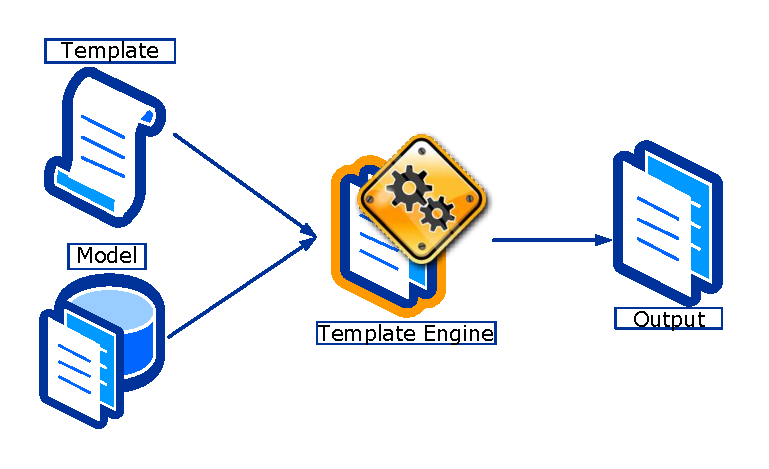
\includegraphics[scale=0.8]{images/TemplateGeneration.pdf}}
    \caption[Template engine]{Figure shows a conceptual view of a template engine.}
    \label{fig:template_engine}
\end{figure}
Figure~\ref{fig:template_engine} depicts the idea behind a template engine. You have some kind of data source (e.g. a model) which get matched towards a template that have markers on where to insert data. After the compilation, the engine outputs what is defined in the template.

\subsubsection{JET}
Java Emitter Templates is a template engine in the M2T (model-to-text) project within the Eclipse ecosystem. JET provides a well known syntax based on JSP, which  has a standard tag library included, that can be extended with custom tag libraries. It comes with editor support and integration with the Eclipse UI.

\lstset{caption=Simple example showing the JSP like syntax in JET,label=list:jetexample,captionpos=b}
\begin{table}[htbp]
  \centering
\begin{lstlisting}[showstringspaces=false]
<%@ jet package="generator.dpf"
  class="DpfGen" 
  imports ="generator.dpf.blog.Article no.hib.dpf.core;"
%>
<% Article art = (Article)argument;%>
public class <%=art.getName()%> {
    public <%=art.getName()%>() {

    }
}
\end{lstlisting}
\end{table}

Listing \ref{list:jetexample} shows a very basic example on how a JET file could look like. We also see that objects are used directly, and not interpreted as the generator frameworks.

\subsubsection{Apache Velocity}
Velocity shares a lot of the same properties that JET possesses. The main difference is the template language, where Velocity provides its own. The language is simple, yet powerful, and provides the same functionality that JET can offer. If the standard functionality is not enough, there are sub-projects like VelocityTools that solves problems like date and number formatting, math operations and more. There is a strong focus on separating code from the templates, thus enforcing patterns like MVC. There is no editor support for Eclipse out of the box, this is achieved using third party plug-ins. 

\lstset{language=HTML,caption=Example showing the Velocity template language,label=list:velocityexample,captionpos=b}
\begin{table}[ht]
  \centering
\begin{lstlisting}[showstringspaces=false]
<HTML>
<BODY>
Hello $customer.Name!
<table>
#foreach( $mud in $mudsOnSpecial )
   #if ( $customer.hasPurchased($mud) )
      <tr>
        <td>
          $flogger.getPromo( $mud )
        </td>
      </tr>
   #end
#end
</table>
\end{lstlisting}
\end{table}

\subsection{Code Generation Frameworks}
A code generation framework is more than a simple template engine. The biggest difference lies with the additional tooling around the engine, like debugging, editor support and profiling of templates. The problem identified in section~\ref{sec:metamodels_and_cg} is addressed in these tools through a built-in interpreter which interprets the DSML, and creates a template editing environment where the editor support reflects the domain concepts of the DSML.

\subsubsection{Acceleo}\label{subsec:acceleo}
Acceleo~\cite{acceleo} is the product of Obeo, the same company that is behind Obeo Designer. The project has been in development 
since 2006, and was incorporated into the Eclipse M2T project in 2009. Acceleo is the reference implementation of 
Object Management Group's MOF model to text transformation language (MOFM2T)~\cite{MOFM2T}. It has full integration with EMF, 
which means you can use Ecore, UML2, etc. The framework has support for debugging and profiling templates, as well 
as editor support with auto completion and content assist. The debugger has its own Eclipse view where you can debug the templates directly using breakpoints. You can also step over/into/return functions like Eclipse JDT provides for Java. 

Another notable feature is the generator module system. A generator module is a plug-in with pre-defined generator templates for a particular domain. This enables the users of Acceleo to take advantage of available generators for popular domains. The drawback of this system is that the generators are (of course) bound to a specific type of metamodel, and might not be tailored to the specified requirements.

\lstset{caption=Example showing the MOFM2T language used in Acceleo,label=list:acceleoexample,captionpos=b}
\begin{table}[ht]
  \centering
\begin{lstlisting}[showstringspaces=false]
[template public generate(aClass : Class)]
  [file (aClass.name.concat('.java'), false)]
    public class [aClass.name.toUpperFirst()/] {
    [for (p: Property | aClass.attribute) separator('\n')]
      private [p.type.name/] [p.name/];
    [/for]
  [/file]
[/template]
\end{lstlisting}
\end{table}

\subsubsection{Xpand}
Xpand~\cite{xpand} is a framework under the Eclipse M2T project that facilitates MDE activities such as code generation, model validation and model transformations. The company behind Xpand is Itemis~\cite{itemis}, a german consulting company focusing on utilizing MDE in projects. Xpand has a wide variety of features which makes it a good fit for this projects requirements. Most notably, you can create editors (with code completion and syntax highlighting) from metamodels specified in EMF Ecore, UML2, XSD and JavaBeans. Besides the predefined metamodels, it is possible to define a custom metamodel that is based on an arbitrary modelling language. Xpand is discussed in detail in section~\ref{sec:xpand}\newline

\subsubsection{Comparison}
Table \ref{tab:gen_features} gives an overview of the different features in the evaluated solutions: 
\begin{description}
  \item[Template Language] The language used in the templates.
  \item[Editor Support] All the considered solutions provide some kind of editor support with syntax highlighting and template validation. The difference from the template engines to generator frameworks lies with how this editor support is provided. Xpand and Acceleo interprets the input models and provide an environment for creating templates, extensions and validation based on the metamodel. In a DPF context this means you operate on the concepts of the DSML, rather than the instance model's actual Java objects. This is discussed in detail in section \ref{sec:xpand}.
  \item[Custom Metamodel] Xpand and Acceleo provide support for EMF and UML models out of the box. This means an UML model will act as a metamodel, i.e. expose its domain concepts in the editor environment. This is discussed in detail in section \ref{sec:xpand}.
  \item[Profiler/Debugger] Profilers are used to optimize your templates and extensions, and gives an overview of which parts of the system that is slow. Both Acceleo and Xpand has a profiler.
  A debugger is useful for finding bugs inside the templates. Acceleo allows you to debug templates like Java classes in Eclipse, with a debug view, breakpoints and stepping over/into/return functions.
\end{description}
\let\Oldarraystretch\arraystretch
\renewcommand*\arraystretch{1.5}

\begin{table}[htb]  
  \centering
  \resizebox{1\textwidth}{!}{
    \begin{tabular}{|p{32mm}|p{22mm}|p{27mm}|p{27mm}|p{27mm}|}
      \hline
      \textbf{Tool}                   & \textbf{Template\newline Language}  & \textbf{Editor Support}  & \textbf{Custom\newline Metamodel} & \textbf{Profiler/\newline Debugger}\\
      \hline
      \textbf{Apache Velocity}       & VTL                   & No                                       & No                      & No \\
      \hline
      \textbf{Eclipse JET}           & JSP                   & No                                       & No                      & No \\
      \hline
      \hline
      \textbf{Acceleo}               & MOFM2T                & Yes                                      & No                      & Yes \\
      \hline
      \textbf{Xpand}                 & Xpand                 & Yes                                      & Yes                     & No \\
      \hline
    \end{tabular}
  }
  \caption {Feature comparison in template engines}
  \label{tab:gen_features}
\end{table}
% template language, profiler, template editor, custom generator metamodel, 
\let\arraystretch\Oldarraystretch
The reason for choosing Xpand is together with the rich tooling, the possibility of creating a custom metamodel. The included profiler is a welcomed feature, but was not critical to the choice of solution. The choice of template language was not crucial either, but a language with its foundation in a standard is a positive trait. Acceleo is providing the same functionality as Xpand with some minor differences in the tooling. A simpler choice would have been either JET or Velocity, but this would be a poor solution for the end-users because of the lack of tooling. Both Acceleo and Xpand provides a "sandboxed" editor environment, which means the template coder only has access to the DSML concepts which is defined through a Xpand/Acceleo metamodel.

\section{Xpand}\label{sec:xpand}
% OAW og naming
Xpand is created and maintained by the german consulting company Itemis~\cite{itemis}. Before the project was included into the Eclipse M2T project, it was called \emph{openArchitectureware (oAW)}~\cite{OAW08Manual}. The functionality is the same, but the project has been split up into different Eclipse projects. Xpand is under the M2T project, while the \emph{Modeling Workflow Engine (MWE)} is under \emph{Eclipse Modeling Framework Technology (EMFT)}. The workflow engine connects the different components in Xpand and executes them. Even though the components have a clear separation, we will use Xpand for all of the included technologies, and explain them when needed.

The biggest difference from a simple template engine, is the built-in interpreter that interprets a DSML and provides functionality based on what a Xpand metamodel dictates. In Xpand, the metamodel is the internal mapping from types in the DSML to types that Xpand understands. Xpand comes with metamodels for the most popular modelling facilities today; EMF, UML2, XSD and plain Java classes. Although these metamodels covers the most used languages, it lacks support for DSMLs specified in anything besides what Xpand has to offer. There are a lot of proprietary DSMLs out there which is not modeled in any of the mentioned languages. Acceleo solves this by saying you need to specify your DSML in EMF/EMOF. This is not a generic solution, and requires the users to create a new EMF/EMOF implementation for each new language that is created. A solution to this problem is to create a model-to-model transformation which can transform your DSML to EMF. The disadvantage is that you are still restricted to the functionality that the Acceleo metamodel defines (which is the EMF concepts), when you perhaps would want to define your own.

DPF is a framework for creating DSMLs, and as discussed in chapter \ref{chap:model_based_development}, DPF Editor falls under the language workbench category. The use case for the DPF project is to generate tooling based on a specified DSML; we want a generic way to define generators for an arbitrary DSML. This use case is a bit narrow, and is probably why Acceleo has not facilitated custom metamodels. Xpand fits our criteria nicely with the ability to create custom metamodels with custom attributes and operations. Xpand lets us create a separate API used only in the templates and extensions, on top of the existing functionality that resides in the DPF Core API. The metamodel defines a mapping from DPF types to Xpand types which is reflected in the template/extension editor. 

Xpand is a feature rich framework with features as \emph{aspect-oriented programming (AOP)}, functional extensions, model-to-model transformations, model-to-text transformations and model validation. The framework provides three different languages that has separate functionality; Xpand, Xtend and Check.
% Noko om namnet
% Må eg sei at metamodel betyr Xpand metamodel?
% javabeans er internal
\begin{description}
  \item[Xpand] \hfill \\
    Xpand is the template language that controls the output of the generator. Apart from the usual control flow statements, it supports lazy evaluation, \codeText{let} statements, aspect oriented programming and extensions created using Xtend and/or Java.
\newpage
\lstset{caption=Example showing the Xpand syntax,label=list:xpandexample,captionpos=b}
% \begin{table}[ht]
%   \centering
  \begin{lstlisting}[showstringspaces=false]
«IMPORT dpf
«EXTENSION org::eclipse::xtend::util::stdlib::io»
 
«DEFINE main FOR dpf::Specification»
  «EXPAND graph FOR this.graph»
«ENDDEFINE»
 
«DEFINE graph FOR dpf::Graph»
  «EXPAND domainclasses FOREACH this.getDomainClasses()»
«ENDDEFINE»
 
«DEFINE domainclasses FOR dpf::DomainClass»
  «syserr(this.name)»
«ENDDEFINE»
  \end{lstlisting}
% \end{table}
    This listing shows a simple template where we traverse our DPF Specification and print out the name of a DSML type called \emph{DomainClass}. We also see how the inclusion of extensions are performed. These extensions are defined in Xtend and/or Java.
  
  \item[Xtend] \hfill \\
    Xtend is used as an extension language. It follows the functional paradigm and provides features like type inference, recursion, caching of methods and calling external Java extensions. It also provides ways to perform model-to-model transformations. This language helps to enforce the separation between program logic and template code; it is strongly encouraged to perform logic in an extension, and call the extension from the template. Such extensions are called \emph{embedment helpers}~\cite{fowler2010domain}.
\lstset{caption=Example showing Xtend extensions,label=list:xtendexample,captionpos=b}
% \begin{table}[ht]
%   \centering  
  \begin{lstlisting}[showstringspaces=false]
importDate(dpf::DomainClass this) :
  if this.getAAttributes().exists(e | e.target.name == "Date") then
	"import java.util.Date;";

String paramList(List[dpf::DomainClass] this) :
  JAVA no.hib.dpf.codegen.generator.extensions.
	StringUtil.getAttributeList(java.util.List);
  \end{lstlisting}
% \end{table}
    Listing~\ref{list:xtendexample} shows the Xtend language, with two Xtend methods. \codeText{importDate} shows how we detect a \emph{Date} type defined in our DPF model. If such a type exists, we return a string that contains an import statement. This example demonstrates the type inference by not declaring a return value. It also showcases some of the functional syntax with the \codeText{exists} statement, which returns a boolean value based on the expression within.
    The last example shows how a Java extension is called from Xtend. Type inference from these extensions are not supported, so we explicitly need to declare the return type. We also observe the need to use fully qualified method names for the extension class. This method in particular returns a \codeText{String} that has been constructed from a list of \codeText{DomainClass} types.
% Reducing \emph{foreign code} in the templates improves readability drastically. 
  \item[Check] \hfill \\
    The Check language handles constraint checking on the model.
\lstset{caption=Example showing a simple constraint check,label=list:checkexample,captionpos=b}
% \begin{table}[ht]
%   \centering  
  \begin{lstlisting}[showstringspaces=false]
import dpf;

context Attribute ERROR
  "Name of " + name + "too short." : name.length > 1;
  \end{lstlisting}
% \end{table}
    Listing \ref{list:checkexample} shows a simple constraint check. The first line imports the metamodel. The second and third line checks the length of property \emph{name} in \codeText{Attribute}, and returns an \codeText{ERROR} if the test fails. Denoting the Check statement with \codeText{ERROR} will abort the workflow and print the error to a console. Alternatively, one can use \codeText{WARNING}, which will print the warning and continue the workflow.
    In the DPF Editor the constraint checking is done within the DPF model, but all validation could happen in the generation phase using Check if desired.
\end{description}
These languages are built upon the same type system, and share a lot of the syntax. The shared syntax is called the \emph{expression sub-language} and provides the basic flow control constructs of all the three languages (e.g. if-conditions, switch statements, casting). The expression sub-language syntax is a mix between Java and OCL.

\subsubsection{Workflow}\label{subsub:workflow}
The Modeling Workflow Engine (MWE) provides a way to execute different Eclipse modelling components in a sequential manner. The execution environment can be inside Eclipse or standalone. Modelling components do not have to be part of the Xpand framework; a component needs to adhere to an interface which MWE provides.

A workflow is defined in a XML file, where each component has its own configuration. Some of the components in Xpand are shown in listing \ref{list:workflowexample}. A workflow do not have to include all of the components shown; a typical workflow for generating code only consists of a reader and generator component.
\newpage
\lstset{language=XML,caption=An example MWE workflow file,label=list:workflowexample,captionpos=b,breaklines=true}
\begin{table}[htpb]
  \centering  
  \begin{lstlisting}[showstringspaces=false]
    <?xml version="1.0"?>
    <workflow>
(1)	    <property name="model" value="path/to/model/Model.xmi" />
	    <property name="src-gen" value="src-gen" />
	    
(2)	    <bean class="org.eclipse.emf.mwe.utils.StandaloneSetup" >
		    <platformUri value=".."/>
	    </bean>
	    
(3)	    <bean id="mm_emf" class="org.eclipse.xtend.typesystem.emf.EmfRegistryMetaModel"/>

(4)	    <component class="org.eclipse.emf.mwe.utils.Reader">
		    <uri value="platform:/resource/${model}" />
		    <modelSlot value="model" />
	    </component>

(5)	    <component class="org.eclipse.xtend.check.CheckComponent">
		    <metaModel idRef="mm_emf"/>
		    <checkFile value="metamodel::Checks" />
		    <emfAllChildrenSlot value="model" />
	    </component>

(6)	    <component class="org.eclipse.xtend.XtendComponent">
		    <metaModel class="org.eclipse.xtend.typesystem.emf.EmfRegistryMetaModel">
			  <metaModelFile value="${model}"/>
		    </metaModel>
		    <invoke value="test::Trafo::duplicate(rootElement)"/>
		    <outputSlot value="newModel"/>
	    </component>

(7)	    <component class="org.eclipse.xpand2.Generator">
		    <metaModel idRef="mm_emf"/>
		    <expand
			    value="template::Template::main FOR model" />
		    <outlet path="${src-gen}" >
			    <postprocessor class="org.eclipse.xpand2.output.JavaBeautifier" />
		    </outlet>
	    </component>
    </workflow>
  \end{lstlisting}
\end{table}

Listing \ref{list:workflowexample} shows a workflow file where an Ecore model is used for input:
\begin{enumerate}
  \item The first lines declares properties for model location and the output folder for the results.
  \item \codeText{StandaloneSetup} is used to initiate EMF specific functionality, like \codeText{platform:/resource} URIs.
  \item Initiation of the Xpand metamodel. The handle \codeText{mm\_emf} is used to refer the metamodel throughout the workflow definition.
  \item The \codeText{Reader} component is used to read the input model's Ecore, and then create a \emph{slot} which stores the model in a named attribute.
  \item This is the configuration of the \codeText{Check} component. We define the EMF metamodel to operate on, as well as the name of the Check file.
  \item The \codeText{Xtend} component performs a model-to-model transformation based on the rules specified in the Xtend file.
  \item The generator component is the one generating code. We start off by defining the EMF metamodel, then we define the entry point in the templates, and also refer the model that the template should be run on. Finally, we define an outlet path where the resulting code should be written to. We also apply a postprocessor to our output, in this case a \codeText{JavaBeautifier}. The \codeText{JavaBeautifier} is a class which format the generator output to our needs. There are postprocessors included in Xpand for C++, Java and XML.
\end{enumerate} 

It is important to point out that the order of the components matter. Before using a Xpand metamodel it is necessary to use its corresponding reader component first (if it has one). Using a metamodel dependent component with an uninitalized metamodel will result in errors.

\begin{figure}[htpb]
  \centering
  \centerline{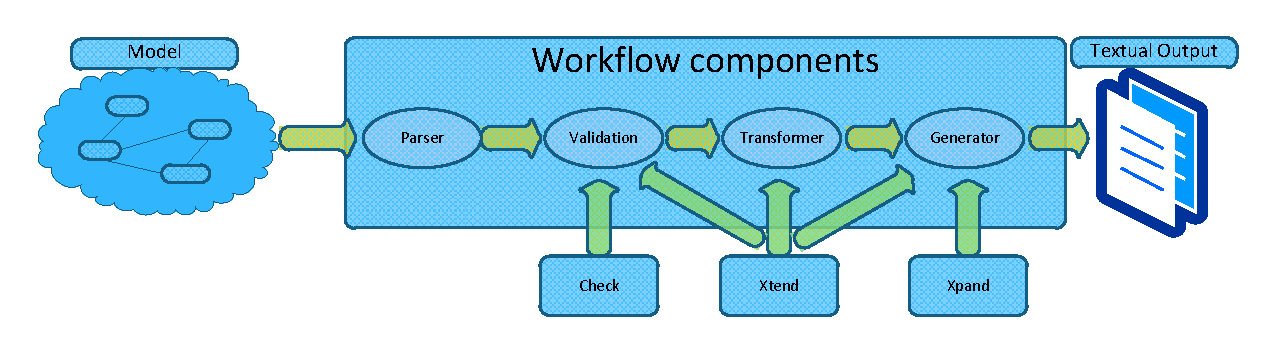
\includegraphics[scale=0.8]{images/xpandworkflow.pdf}}
  \caption[Workflow in Xpand]{Figure shows how the workflow engine works.}
  \label{fig:xpand_workflow}
\end{figure}

Figure \ref{fig:xpand_workflow} depicts a workflow in Xpand. Although a usual workflow, all of the components are optional, and could be replaced by something else.
\newpage
\subsection{Xtend 2}\label{subsec:xtend2}
In December 2011, version 2.2 of Xtend~\cite{xtend2} was released. This is Xpand's successor, and is the main focus for Itemis from now on.  Xpand will be maintained for a while, but will probably be dropped in favour of Xtend 2 in the longterm. 

The naming is a bit confusing, as the Xpand framework has a separate language called Xtend (see listing \ref{list:xtendexample}). Xtend 2 is a complete rewrite and is not compatible with older versions of Xpand. It is based on Xtext~\cite{xtext}, another Eclipse project created by Itemis. Xtext is a language workbench for textual languages where one can create editors and generators from a grammar. Currently Xtend 2 is a part of the Xtext project, but will in time become a separate project. The reason for this re-implementation is mentioned in the lead developer Sven Efftinge's blog~\cite{efftinge_blog}; performance issues, poor tooling and shortcuts in the language.

Xtend 2 is a fully-fledged programming language, which compiles to readable Java code. The language aims to reduce the verbosity of Java, and support features like type inference, closures and operator overloading. Generating code is done through what is called \emph{template expressions}, which is the syntax from Xpand embedded into the Xtend 2 language. Instead of the interpreter based approach of Xpand, the template expressions are compiled to Java code. At the time of writing, Xtend 2 do not provide the same functionality as Xpand as it has no support for loading custom models.

Xtend 2 can work on a grammar defined in Xtext, which in its turn has its foundation in EMF Ecore. More information on this works can be found in the Xtext/Xtend documentation~\cite{xtend_codegen}. Further information on Xtend 2 can be found at Xtend web site, and Sven Efftinge's blog as well ~\cite{xtend2}~\cite{efftinge_blog}.

% Det er mogleg med interpreters i xtext
% Lage figur som viser korleis ein får editor support frå Xpand metamodel
% http://www.eclipse.org/forums/index.php/m/798256/#msg_798256
%     \item Xpand successor: http://blog.efftinge.de/2010/12/xtend-2-successor-to-xpand.html
%     \item Xpand artiklar: http://blog.efftinge.de/search?q=xpand
% http://www.eclipse.org/Xtext/documentation/2_0_0/040-first-code-generator.php
% http://www.eclipse.org/Xtext/documentation/2_0_0/210-emf-integration.php#emf_codegen
% Xpand interpreted
% Xtend compiled
\chapter{Design and Development}\label{chap:design_and_development}
This chapter gives an in-depth look at how the implementation of the code generation tool works, and how it fits together with the DPF Editor and the Xpand framework. The different components and their function will be explained. In the end of the chapter there will be an overview of what has been achieved throughout the development, and what the tool's shortcomings are.

In the Xpand documentation, the mapping between a DSML and the Xpand types are referred to as the metamodel. Hence we will use \emph{metamodel} when describing the \emph{DPF Xpand type mapping}. When referring to the Ecore metamodel in which DPF is specified, we will describe it as \emph{DPF Ecore metamodel}. 

\section{Development Process}
\subsubsection{Development Methodology}
This project has chosen to use \emph{Agile} development methodologies. The methodology chosen for this project is Extreme Programming (XP), although following it completely by the book has not been possible. XP was created by Kent Beck~\cite{Beck:2004:EPE:1076267} which is one of the pioneers in the Agile movement~\cite{agile_alliance}. The reason for choosing XP over other agile methodologies is that it is tought in the MOD251 class at Bergen University College. There are a few constraints which hindered following XP properly; the project had no clearly defined requirements, lack of time and no one else working on the same problem (pair-programming).

In the development phase of the project, the aim was to deliver working software every two weeks coinciding with DPF project meetings. The meetings gave a chance to review what had been done, and the focus area for the next iteration.
  
% Even though some of the 
% \begin{itemize}
%   \item Methodology
%   \item Infrastructure, trac
%   \item No tdd, time
%   \item Learning project. Ingen visste noko om verktøy og korleis ting skulle sjå ut. Difor vanskelig med klar prosess.
% \end{itemize}
\subsubsection{Coding Convention}
XP dictates that one should use a predefined coding convention before starting the development. Such standards aim to result in code that is consistent from developer to developer. It defines how the code looks, but can also include guidelines on which patterns to use and avoid. Although this project was developed by one developer, it needs to be maintained by someone else in the future.
   
The code convention used in this project is Eclipse Naming Conventions~\cite{eclipse_naming_conventions_web}. This convention defines how Eclipse specific elements should be named (e.g. plug-ins and package names). The code convention in general uses Oracle's own guidelines~\cite{java_naming_conventions_web}. The reason for choosing these conventions are that the DPF Editor itself uses them throughout, as well as beeing de-facto standard in the Java ecosystem. Having a completely consistent codebase will improve readability and thus make it easier for new project participants to get started.
  
\subsubsection{Tools}
The development process has been aided by different tools to create an environment which enhances productivity and provides structure. An important tool, even when programming alone, is a bug tracker. Using a bug tracker helps structuring ideas, as well as keeping track of defects. The tool chosen for this task was Trac~\cite{trac}, a lightweight Python based bug tracker with wiki functionality, integration with version control systems (VCS) and the possibility of creating milestones from feature requests and bugs. Along with Trac, Mercurial~\cite{mercurial} was chosen as the VCS. 

The development process was aided by the Eclipse Modeling Tools (Eclipse Java Development Tools with modelling components), using the latest version \emph{Indigo} (3.7)~\cite{Eclipse}. The metamodel is based on the latest released Xpand SDK (1.1.1) which can be found in the modelling components installer inside Eclipse. Logging is used throughout the project for debugging purposes. The logging facility used is called Apache Log4j~\cite{l4j}.

\section{Project Overview}
\subsubsection{Naming Components}
This project uses the same naming conventions which the DPF Editor code base uses. This means all packages starts with \codeText{no.hib.dpf} to denote it is a part of the DPF project. As the sub-project name, \codeText{codegen} is chosen. In time there might be other code generation solutions based on other frameworks than Xpand, and it is suitable to put such projects under the same name. Furthermore, as a component name, \codeText{xpand} is chosen. This is to denote that the particular solution is based on Xpand. \codeText{metamodel} is chosen as sub-component name following the convention used in the Xpand project.
  
The following plug-in projects are defined:
\begin{description}
  \item[\codeText{no.hib.dpf.codegen.xpand.metamodel}]
  \item[\codeText{no.hib.dpf.codegen.xpand.metamodel.test}]
  \item[\codeText{no.hib.dpf.codegen.xpand.metamodel.ui}]
\end{description}
    
% Figure~\ref{fig:dpf_workbench_overview} shows the current architecture of the tools in the DPF Editor, included the code generation component described in this chapter (denoted Xpand and Xpand Extensions).
% 
% \begin{figure}[htpb]
%   \centering
%   \centerline{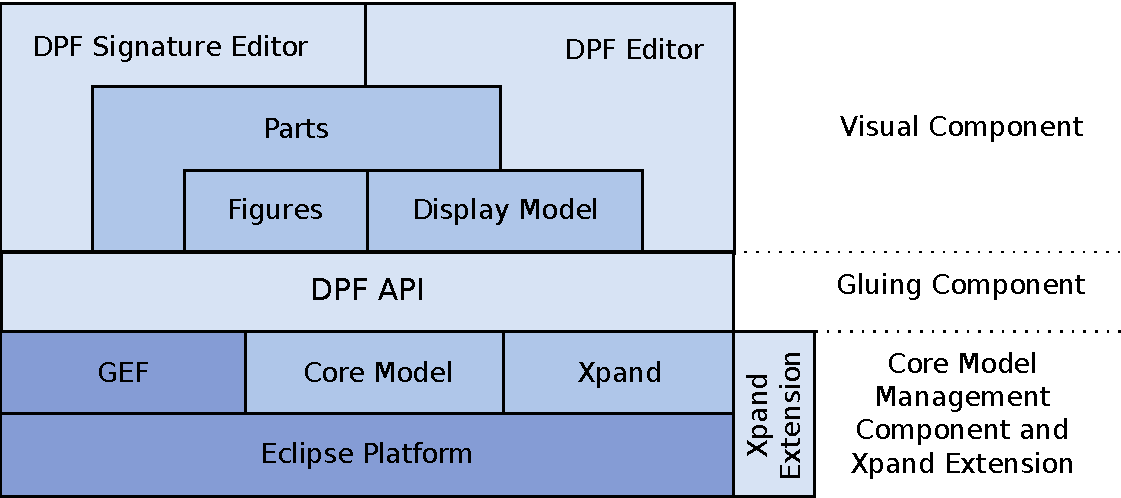
\includegraphics[scale=0.5]{images/component_architechture_r.pdf}}
%   \caption[DPF Editor Architecture]{Architecture of the DPF Editor.}
%   \label{fig:dpf_workbench_overview}
% \end{figure}
% 
% Kodegenerering pluggable component

\section{Problem Description}\label{sec:problem_description}
As discussed in section \ref{sec:metamodels_and_cg}, the DPF Editor is in need for a general solution to creating code generators. Using regular template engines will result in a code generator that would not convey the domain concepts of a DSML. An ideal solution would have the following traits:
\begin{description}
  \item[Clear expression of domain concepts] \hfill \\
  The concepts of the DSML should form the basis for the constructs used in creating templates.
  \item[Integration with Eclipse] \hfill \\
  Editor support is an important feature which makes the template creation process more user-friendly and intuitive. Features like template debugging and profiling are features which also improves the user experience with the tool.
  \item[Standalone generator] \hfill \\
  A generator which does not have to many dependencies are more portable and reusable. With dependencies directly on Eclipse, one would make the solution hard to use in other contexts.
\end{description}

These goals are more or less already achieved in Acceleo and Xpand, but only for the predefined model types which are EMF, UML2 and XSD. This chapter will describe a solution that facilitates the use of DPF models in a custom Xpand metamodel.

\lstset{caption=An example of a Xpand template using the DPF Ecore metamodel as basis.,label=list:xpand_domainconcept,captionpos=b}
\begin{table}[ht]
  \centering
\begin{lstlisting}[showstringspaces=false]
«DEFINE gettersAndSetters FOR core::Node»
	«IF this.getTypeName() != "DomainClass"»
		public «this.getTypeName()» «getter(this)»() {
			return «this.name.toFirstLower()»;
		}
	«ELSE»
		public «this.name.toFirstUpper()» «getter(this)»() {
			return «this.name.toFirstLower()»;
		}
	«ENDIF»
«ENDDEFINE»
\end{lstlisting}
\end{table}

Listing~\ref{list:xpand_domainconcept} shows an example where we use the DPF Ecore metamodel with the EMF metamodel. For each \codeText{DEFINE} block in the templates we need to iterate over \emph{all} nodes of the DPF model, and not the particular collection of nodes conforming to a metatype. This example shows the creation of Java \emph{get} methods from a DSML which contains a \codeText{DomainClass} entity. What we want to achieve is a \codeText{DEFINE} block where we iterate over \emph{only} the nodes that conforms to the \codeText{DomainClass} metatype.

\section{Metamodels in Xpand}
The introduction of this chapter mentions that metamodels in Xpand are a mapping from types in an actual model language (like Ecore) to the Xpand type system. This naming is somewhat confusing, but one can think of it as a metamodel for Xpand's understanding of a model. The metamodel dictates how the input model should be mapped to the Xpand type system, and what kind of mapping this is.

As stated in section \ref{sec:xpand}, Xpand supports a number of predefined metamodels, namely UML2, EMF, XSD and Java beans. Besides these, we have the built-in Xpand types which also can be regarded as a metamodel. In a MWE workflow (from now referred to as workflow, see~\ref{subsub:workflow}) one can take advantage of multiple metamodels at the same time, making each metamodel handle different aspects of the model. 

An important note is that the order of the metamodels is crucial. As an example we can define a workflow which uses three different metamodels (from the Xpand documentation~\cite{xpand}): 
Let us assume that our model element is an instance of the Java type org.eclipse.emf.ecore.EObject and it is a dynamic instance of an EMF EClass Car.
\begin{itemize}
  \item Built-in metamodel (always first)
  \item Java beans metamodel
  \item EMF metamodel
\end{itemize}
If we want to match \codeText{Car} against \codeText{EObject} in the EMF metamodel we bump into a problem: the first match we get is from the built-in metamodel where we get the Xpand type \codeText{Object}. This is now our \emph{best-fit} as every metatype has to extend \codeText{Object}. We then proceed to the Java beans metamodel which will return a \codeText{org::eclipse::emf::ecore::EObject} which is a specialized version of \codeText{Object}. The EMF metamodel would have returned \emph{Car}, but was unable as we got a match before the metamodel was queried. This example illustrates how important the proper order of metamodels is. If we had changed the order of the Java beans metamodel and EMF metamodel, the proper value would have been resolved. Note that using e.g. a UML2 and EMF metamodel to handle different parts of a model is a rare scenario. The example shown is relevant because most metamodels take advantage of the JavaBeans metamodel to provide functionality in a Java class without the need for any hand coding.

Figure~\ref{fig:xpand_overview} shows how Xpand works in principle. The figure shows how the DSML initializes one or more metamodels which creates custom Xpand types (henceforth referred to as types). More specifically, the DSML are \emph{interpreted} at runtime by Xpand and mapped to types defined in the metamodel. When the workflow is executed, Xpand will parse and validate the templates, this is done with the help from the metamodel which decides which types should be applicable where. When the code generation phase starts, Xpand will match a defined input model against the template. This is done through calls against the metamodel as well.

\begin{figure}[h]
  \centering
  \centerline{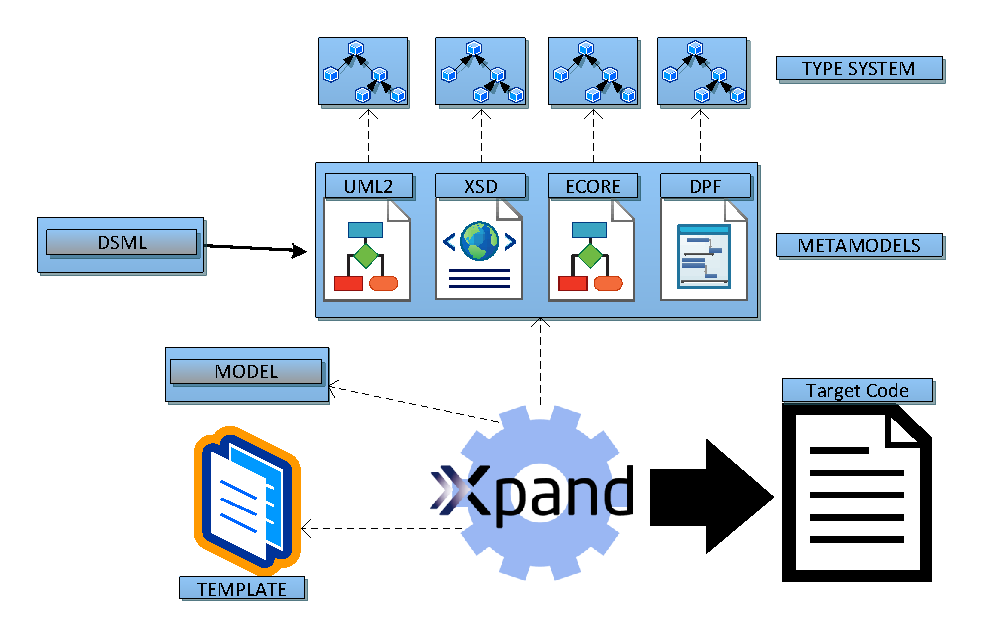
\includegraphics[scale=0.7]{images/xpand.pdf}}
  \caption[Xpand metamodels]{Figure shows how the Xpand metamodels work.}
  \label{fig:xpand_overview}
\end{figure}

A metamodel in Xpand must implement the \codeText{MetaModel} interface. The most important methods that needs implementing are the following:
\begin{description}
  \item[\codeText{getKnownTypes()}] Returns a set of types which represents all of the types the system know of.
  \item[\codeText{getType(Object type)}] Returns a corresponding type which the parameter object is matched against. The objects which is matched against \codeText{getType} are the model objects from either the DSML or instance model. We have to check the object's DPF type to decide how to handle it using the Java operator \codeText{instanceof}.
  \item[\codeText{getTypeForName(String typeName)}] When processing a template, there are type identifiers in the different statements. An example of this is:
  \begin{plainlisting}
«DEFINE test FOR my::namespace::StateType»
  \end{plainlisting}
  The type identifier \codeText{my::namespace::StateType} would be queried against the metamodel to retrieve its designated type, or create a new type if it do not exist.
  \item[\codeText{getNamespaces()}] Returns a set of strings which defines what namespaces the metamodel should handle.
\end{description}

% - figur som viser modell -> interpreter -> conforms til metamodell (vis alle typar) -> lagar typar... conceptual model
% - figur som viser DPF model/metamodel -> DPF Xpand metamodel (Vis internal mm og internal m) -> types?
% -
\subsection{The Xpand Type System}\label{sub:type_system}
The purpose of the type system is to create a common representation of the input models, which can be used as a basis for creating tooling. I.e. rather than creating specialized solutions for a particular model type, we have a general "model" to adhere to. Creating types is also a way to extend the existing functionality in a model; the type system is a \emph{reflection}\footnote{Reflection is the process of dynamically load classes and functionality at runtime.~\cite{reflection_tutorial}} layer which can be extended with the implementation of metamodels. A type in Xpand contains a name, properties and operations, as well as information about inheritance. The type system in Xpand provides access to types based on the metamodels which are used.

Names have the option of using namespaces, which are delimited using "::". In the EMF metamodel, the package name(s) in a model is used as the namespace(s). E.g. with the DPF Ecore metamodel one would have \codeText{no::hib::dpf::core} as the namespace prefix to a type. When using these types in the templates one can import the namespace so that the namespace prefix can be omitted.

When creating a metamodel for Xpand, the types may contain primitives, like string, integer or floats. These types can be wrapped in a tailored solution, e.g. creating a type for floats with operations focused on a particular domain like finance. Often the existing functionality is the best fit to handle primitives as Xpand contains additional functionality for the primitives string, boolean, real and integer. The string class in particular provides methods that is useful in a code generation context, like the "+" operator for string concatenation, regular expressions and more. In addition to the primitives, Xpand has defined a few collection types: Collection, List and Set which corresponds to their Java counterpart (\codeText{java.util.*}). To implement a general approach for the collection types, Xpand uses the concept of \emph{parameterized types}\footnote{A parameterized type in Xpand is a type which has an inner type. The inner type defines what type a collection can contain and must be a Xpand type.}.

As mentioned a Xpand type contains properties and operations based on reflection. Along with static properties, they are what is called \emph{features}. 
\newpage
The features are defined as following:
\begin{description}
  \item[Attribute] \hfill \\
  An attribute contains a name and a return value which is another type.
  \item[Operation] \hfill \\
  An operation is structurally identical to Attributes with the addition of parameters.
  \item[Static Property] \hfill \\
  A static property provides the same functionality as enums or constants. It has no parameters.
\end{description}

In Ecore, every attribute can have a specified type (like \codeText{EString}), and the \codeText{EClasses} can inherit a super-type. When mapping types which have its foundation in a Java class, we can take advantage of the JavaBeans metamodel for providing the functionality it contains. Instead of defining the JavaBeans metamodel within the workflow, it is possible to use it directly in our own metamodel. E.g. the EMF metamodel relies on the JavaBeans metamodel for handling types which is external to the Ecore model.

\section{DPF Xpand Metamodel}
As the problem description (\ref{sec:problem_description}) suggests, using the DPF Ecore with the Xpand EMF metamodel will result in a tedious and unintuitive solution that does not convey the domain concepts of a DSML. As the predefined metamodels do, the DPF metamodel must implement the \codeText{MetaModel} interface. The DPF metamodel behaves like any other metamodel, and can be used in the same manner. Although not properly tested, the metamodel should work seamlessly with all of the predefined components in Xpand.

\subsection{Considered Approaches}\label{subsec:considered_approaches}
Before initiating the work on creating a Xpand metamodel, a different approach was considered due to the high learning curve of Xpand's internals. Since EMF is supported "out of the box", the first thought was to create a model-to-model transformation from DPF to EMF. This approach is valid, but as we discussed in section \ref{sec:xpand} it would restrict the functionality provided to what was defined in the EMF metamodel. A model-to-model transformation from DPF to EMF is probably work worth a master's thesis by itself, and was thus not considered to be a viable solution. 

Another approach considered (see figure~\ref{fig:xpand_dpf_m2m}) was a simplified model-to-model transformation where an Ecore model was built programmatically from a DPF specification focusing on the basic constructs like nodes and arrows. To make this work, we would have to create an (dynamic) Ecore model on the fly and generate a .ecore file which would provide editor support. To make things worse, dynamic EMF does not support creating custom operations like regular EMF does. The biggest problem with this approach however, is that the operations which would be provided through Xpand, would be the generic EMF API. This means we would be back to comparing \codeText{EClass} entities with their name to find a specific DSML node and thus provide no benefit at all.

\begin{figure}[htpb]
  \centering
  \centerline{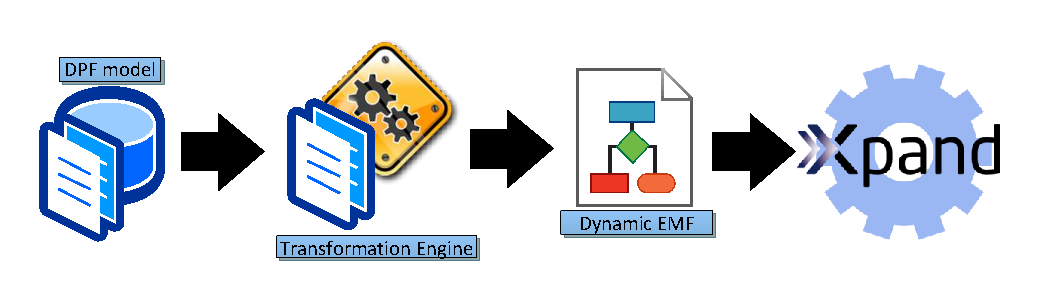
\includegraphics[scale=0.8]{images/dpf_to_emf.pdf}}
  \caption[Model-to-model tranformation from DPF to EMF]{Figure shows the idea behind one of the considered solutions.}
  \label{fig:xpand_dpf_m2m}
\end{figure}

% m2m->emf->xpand->output figur?

\subsection{Packages}
The basic structure of the \codeText{no.hib.dpf.codegen.xpand.metamodel} project contains four different packages.
\begin{description}
  \item[no.hib.dpf.codegen.xpand.metamodel] \hfill \\
  Contains the metamodel class which perform and store all the mappings towards our custom types. It also contains an interface which defines the names of the entities in DPF (e.g. Node, Constraint, Arrow etc.).
  \item[no.hib.dpf.codegen.xpand.metamodel.typesystem] \hfill \\
  The type system package contains utility functionality which are used by the type classes and other parts of the system.
  \item[no.hib.dpf.codegen.xpand.metamodel.typesystem.types] \hfill \\
  This subpackage contains classes for all the custom types. This package is internal, and is not exposed to other plug-ins.
  \item[no.hib.dpf.codegen.xpand.metamodel.workflow] \hfill \\
  This package contains the workflow component \codeText{DpfReader} which handles the initialization of the metamodel, i.e. it loads the DSML's and the model's specification.
\end{description}

\subsection{Structure of the Metamodel}
A way of looking at the metamodel is a black box where you insert the DSML and its instance, and are then able to query it with objects or names which then returns a corresponding type.

\begin{figure}[htpb]
  \centering
  \centerline{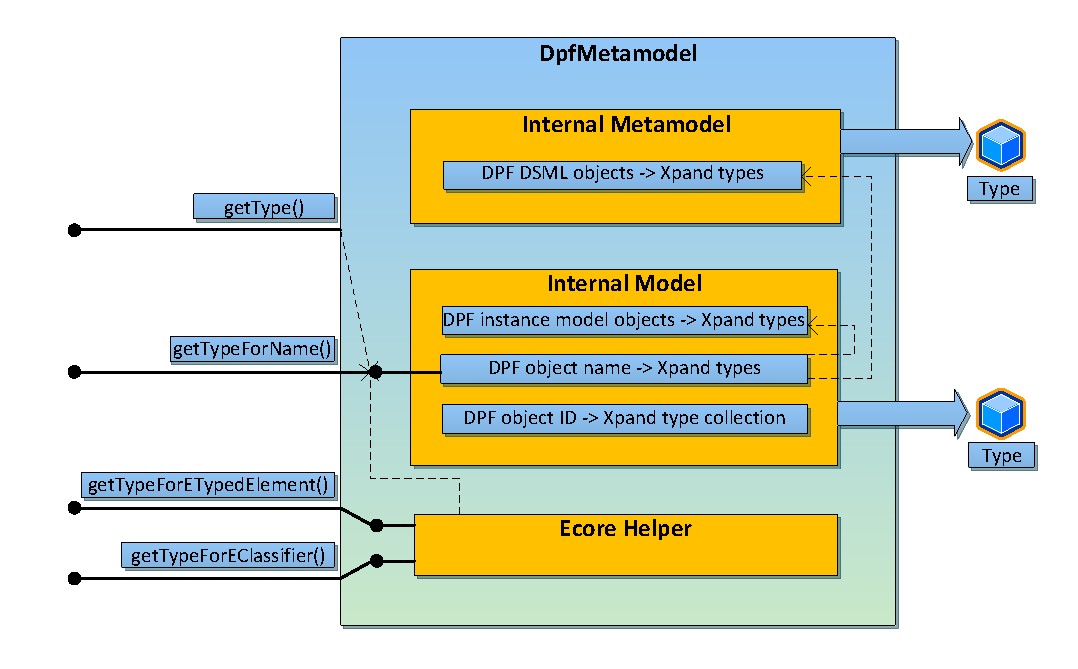
\includegraphics[scale=0.8]{images/metamodelcomponent.pdf}}
  \caption[View of the structure of the metamodel]{Figure shows the internals of a DPF metamodel.}
  \label{fig:metamodel_component}
\end{figure}

The metamodel class has three internal classes with their own responsibility. Figure~\ref{fig:metamodel_component} shows a \emph{internal metamodel}, an \emph{internal model} and what is called the \emph{Ecore helper}. The predefined metamodels in Xpand usually match an object to its metaobject and return that, but in DPF we have a lot of idiosyncrasies which makes it easier to have a representation of the model as well. An important observation is that every call to the metamodel will ultimately go through \codeText{getTypeForName}, and return a result from the internal metamodel \emph{or} the internal model.

There is no validation of the models implemented in the metamodel. The DPF Editor enforce the consistency and validity of the DSML's typing through checking for graph homomorphisms~\cite{Bech11}. Even though we reflect both the DSML and instance model in the metamodel, we do not check for graph homomorphisms between them. When a DSML or instance model is used within the metamodel it is assumed to be valid, both concerning constraints and typing.

\subsubsection{Internal Metamodel}
The internal metamodel represents the DPF DSML and its concepts. When the method \codeText{addDpfMetaModel(Specification)} is called, the \codeText{Specification} object representing the DSML is iterated over, and each DPF type gets matched through a map structure called \codeText{metaModelCache}. This particular mapping is mapped with the DPF model objects from the DSML as keys, and a corresponding type as value. If the type does not exist, a new one will be created with the DSML entity's name as name. In addition to the DSML types, we add two "dummy types", namely \codeText{Node} and \codeText{Arrow} for reasons explained in the next section. Each DSML entity gets stored with its namespace prefixed, although it is hardcoded for DPF models at this point (see~\ref{subsub:namespaces}).
\begin{figure}[h]
  \centering
  \centerline{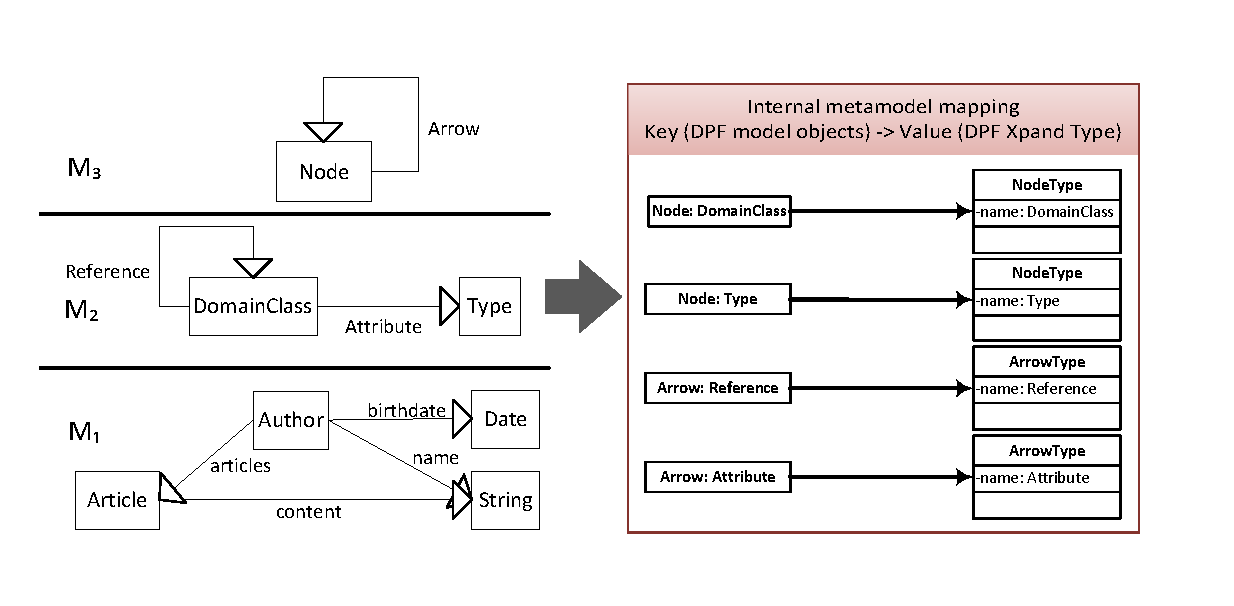
\includegraphics[scale=0.8]{images/dpf_to_type_mapping.pdf}}
  \caption[Mapping from DPF types to DPF Xpand metamodel types]{Figure shows a simple mapping between a DSML and Xpand types.}
  \label{fig:dpf_to_type_mapping}
\end{figure}

Figure~\ref{fig:dpf_to_type_mapping} shows how a simple DSML is mapped to corresponding types within the type system. 

\subsubsection{Internal Model}
An internal model represents the DPF instance model of the DSML. This class is initiated when \codeText{addDpfModel(Specification)} is called. As with the internal metamodel, we create a object to type mapping, but this time with the instance DPF specification as the basis. The reason for mapping the instance model is that we need to retrieve the correct object when traversing the graph. When chaining method calls, we would have returned the DSMLs objects rather than the instance, thus looking up the wrong objects in the metamodel.

Next we create a DPF type ID\footnote{Each node, arrow, constraint and graph has a unique id within the \codeText{Specification} object.} to list of DPF objects mapping. The list of objects is built using all the objects in the instance model which has the same metatype (ID). This is not necessary, but retrieving all instances of a DSML type is a common operation, and a collection simplifies that process. 

The last and most important mapping is the type name to type mapping, which is used for resolving every query to the metamodel. This mapping points to both the internal metamodel mapping \emph{and} the internal model's DPF object to type mapping. As figure~\ref{fig:metamodel_component} shows, the Ecore helper also uses the name to type mapping. Using names to identify objects is unfortunate due to its ambiguity, but necessary as all type definitions in the templates are simple names. An example issue is when nodes and arrows, or more than one node or arrow has the same name: which type is the correct one? The only way to deal with this is to check if the object retrieved from a mapping corresponds with what is queried. The type names are stored with their respective namespace prefix.

\subsubsection{Ecore Helper}
For convenience purposes we take advantage of the functionality specified in the DPF Ecore metamodel. From the types created for the metamodel this helper class gets called to resolve attributes and operations on the \codeText{EClass} in which any DSML/model type is an instance of. It is very useful to get operations like \codeText{get/setName} or \codeText{get/setGraph} for "free", i.e. without having to define them manually in the types. The names of getters are shortened to "name" instead of "getName" for convenience.

\subsection{Type System}\label{subsec:type_system}
The types created for our metamodel reflects the types which DPF defines. The purpose of the types is to encapsulate the model object and expose its functionality through the Xpand type system. As stated in section \ref{sub:type_system} we can also define our own functionality through the Xpand API. This proves to be quite useful, as the DPF API is not tailored for graph traversal and code generation. As an example, we can take outgoing arrows from a node in the DPF Ecore metamodel where the only possibility is to retrieve \emph{all} the outgoing arrows. When writing templates it is convenient to not iterate over \emph{all} the arrows and decide its type within the template itself, as this would create a lot of complexity. A possible solution could be to create an extension that built collections of arrows upon generator execution, but this would be a lot of manual labour and unnecessary because it can be automated. This is where our custom types come to the rescue; we simply define new methods that can be used within the template environment. This particular example problem is tackled by creating a mapping from a DSML type ID to a collection of instance model nodes that has the same metatype ID (see previous section). 

\begin{figure}[htpb]
  \centering
  \centerline{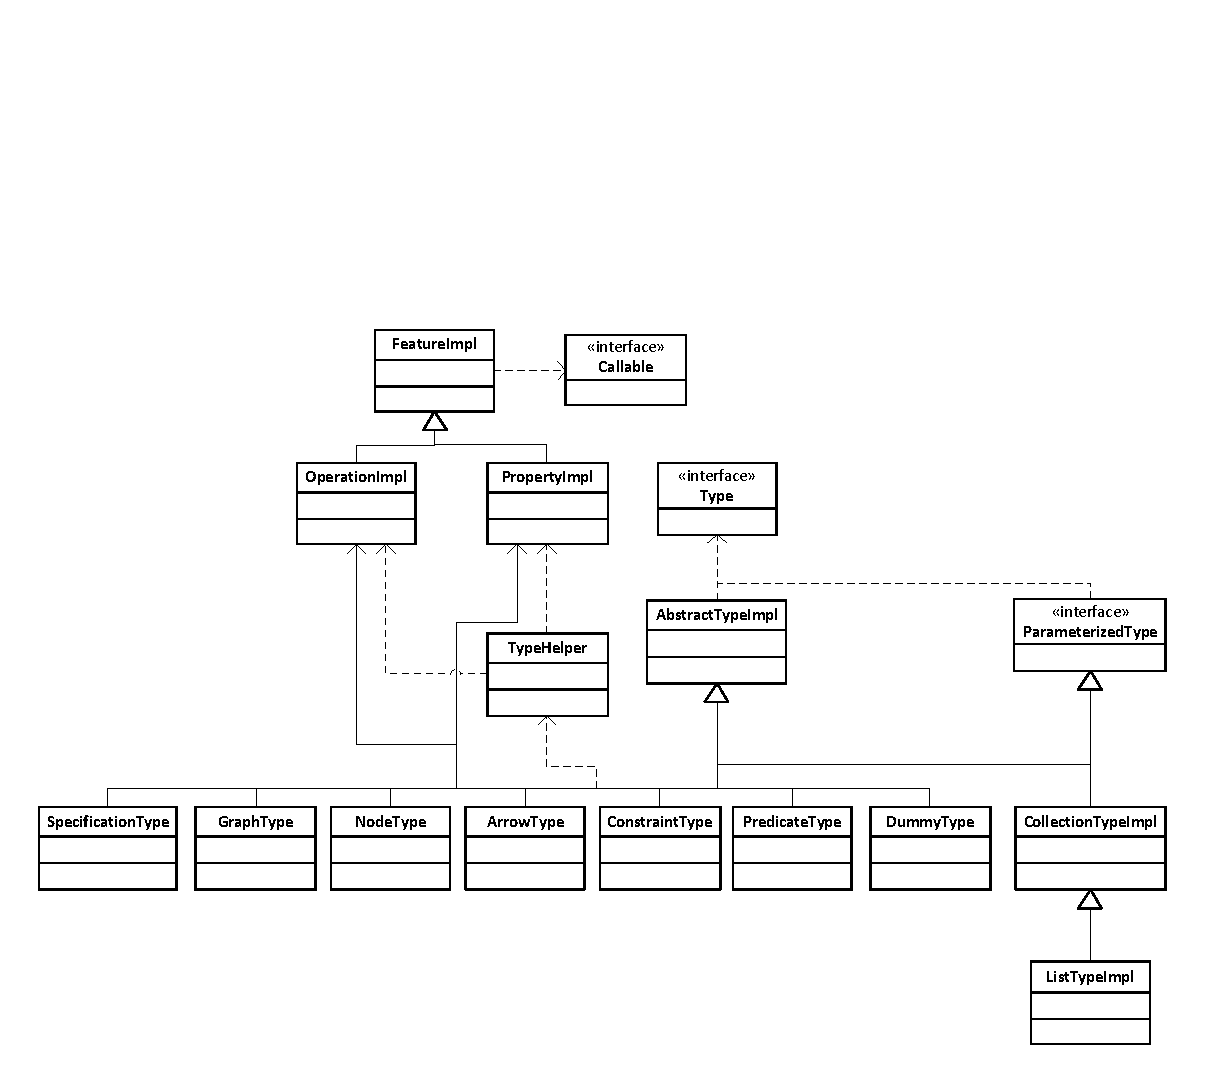
\includegraphics[scale=0.8]{images/typeuml.pdf}}
  \caption[DPF Xpand types]{Figure shows the type system in the DPF Xpand metamodel.}
  \label{fig:xpand_dpf_types}
\end{figure}

Figure~\ref{fig:xpand_dpf_types} shows an overview of the DPF metamodel's typesystem. For each DPF concept, we have a corresponding type. All of the types inherits \codeText{AbstractTypeImpl} which in its turn implements the \codeText{Type} interface. We also see that the \codeText{CollectionTypeImpl} implements the \codeText{ParameterizedType} interface which defines an inner type of the collection, which is how parameterized types are declared in Xpand. As in the \codeText{java.util} package, the list and set is a specialized case of a collection.

We also see that we have referenced attributes, operations and static properties from our types. \codeText{AbstractTypeImpl} does caching of all the \emph{features} within a type automatically. The \codeText{TypeHelper} class is responsible for creating all the Ecore features for each type based on the DPF type. I.e. an instance of \codeText{Arrow} will provide getters and setters for names, retrieving its graph, target and source etc.

Not all of the custom types provide any alterations to their corresponding DPF entity's type. \codeText{ConstraintType}, \codeText{PredicateType} and \codeText{SpecificationType} are only defined through the functionality in the DPF Ecore metamodel. Due to recent API changes there has not been a priority to define custom behaviour as the DPF Ecore functionality is satisfactory.

\begin{figure}[htpb]
  \centering
  \centerline{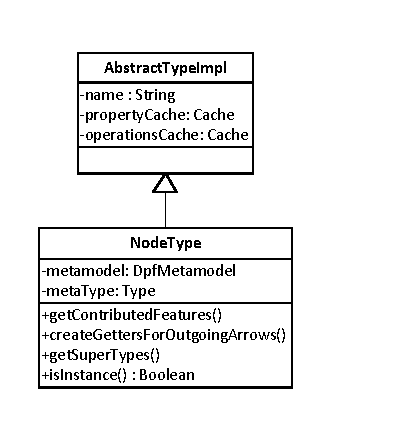
\includegraphics[scale=0.8]{images/nodetypeuml.pdf}}
  \caption[NodeType UML]{A class diagram showing a \codeText{NodeType} and its parent. This graphic only shows selected entities within the classes for simplicity.}
  \label{fig:nodetype}
\end{figure}

Figure~\ref{fig:nodetype} represents a the "anatomy" of a \codeText{NodeType}. All of the specified types for the DPF metamodel inherits \codeText{AbstractTypeImpl}. We see \codeText{AbstractTypeImpl}'s data fields, which contains \codeText{Cache}\footnote{A \codeText{Cache} object is a wrapper around \codeText{java.util.HashMap} with some additional functionality.} objects that store all the \emph{features} of the metamodel. That is, when the method \codeText{getAllFeatures()} is called (which is defined through the Xpand interface \codeText{Type}), the class calls \codeText{getContributedFeatures()} which is an abstract method implemented in the subclass. This is an example of the \emph{template pattern}~\cite{Martin:2003:ASD:515230}.

The Xpand type system supports inheritance within the types. The Java objects which represent the Xpand types has no inheritance in between each other. This inheritance is defined through the method \codeText{getSuperTypes()}, where a type returns a set of Xpand types which the particular type should inherit. In the DPF metamodel each type from the model instance inherits its metatypes's type. Figure~\ref{fig:xpand_dpf_types} shows a type called \codeText{DummyType}, which is a type that only contains its name, no operations and attributes are defined. The reason for implementing this type is to use it as supertypes for the DSML's and instance model's types, for the purpose of defining general methods on e.g. nodes like \codeText{getOutgoingArrows}. Although that particular method is implemented through the DPF Ecore, it will not work due to the DSML and instance model types beeing different from eachother (e.g. a \codeText{NodeType} called \codeText{Process} is not the same type as a \codeText{NodeType} called \codeText{Control}).

The \codeText{createGettersForOutgoingArrows()} is a method which returns custom operations for the node. In short, the method creates a "get" method for each type of arrows which is outgoing from the node. This is the implementation of the scenario mentioned in the beginning of this section.

%dummytype!!!!
% DPF typar som arvar kvarandre
% oversiktsfigur frå nye DPF paper 
% 
% Utfordringar med typar: f.eks Arrow som dummytype, Xpand tek ikkje hand om subtypar.
% Grunn til å bruke model som lag er at ein kan finne kva piler som går kvar når Node.getAttrib()[0].target.Node -> sjekk arrowtype
% \item[\codeText{getType(Object type)}] Returns a corresponding type which the parameter object is matched against. The objects which is matched against \codeText{getType} are the model objects from the DPF \codeText{Specification} object which contains the DSML or model. Every call needs to be handled with the right type in mind because we can not identify the different parts of a DPF model in the same way. 

% typeforname brukt i gettype
\subsection{Reader and Workflow}\label{subsec:reader_workflow}
For the metamodel to work in a MWE workflow, we need a reader component which initates the metamodel with data. In the DPF metamodel's case, we want the reader to load both a DSML and model. A component in Xpand is a class which implements the interface \codeText{WorkflowComponent}. 
% The class consists of a few methods which needs to be implemented

\begin{figure}[htpb]
  \centering
  \centerline{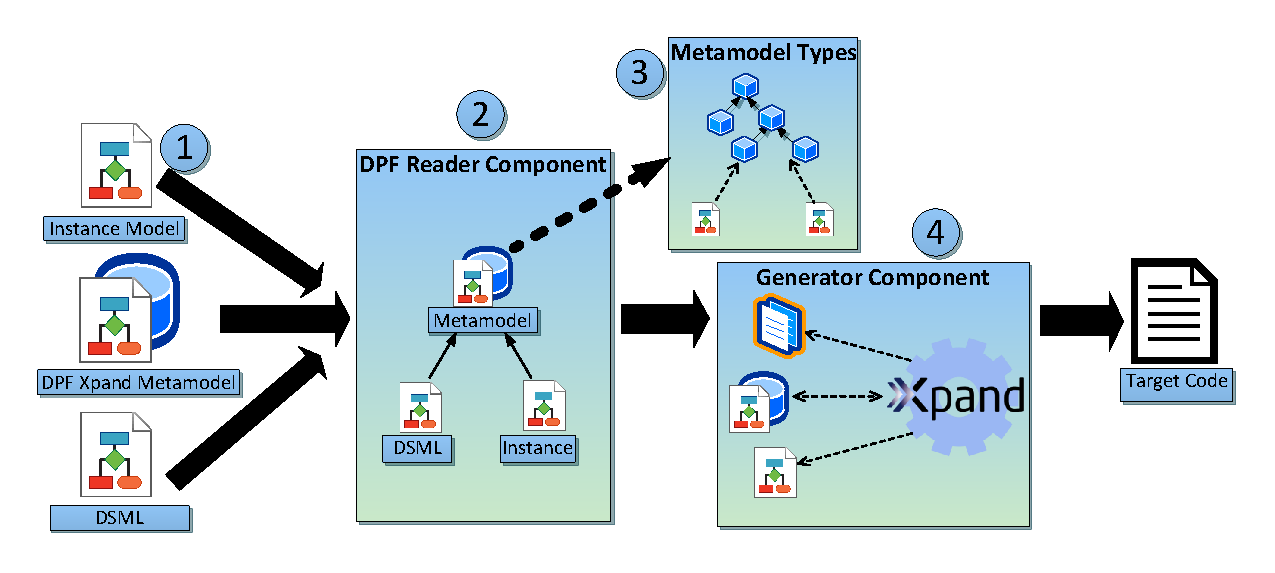
\includegraphics[scale=0.7]{images/xpand2.pdf}}
  \caption[Workflow using the DPF Xpand Metamodel]{Figure shows how the Xpand DPF metamodel works in a workflow.}
  \label{fig:xpand_dpf_workflow}
\end{figure}

Figure~\ref{fig:xpand_dpf_workflow} shows how the workflow proceeds from start to end. This visualization only contains two components, the DPF Reader and the Xpand Generator component.
\begin{enumerate}
  \item The first step in a workflow is to declare properties. We assign a name to e.g. a path or value to simplify the appearance of the workflow file. This is optional as you can use paths directly in the components, the assigned ID is merely an alias. What is important is instantiating the metamodel and assigning it an ID, making it available across components within the workflow. See the three first lines of listing~\ref{list:dpf_component} for example.
  \item The DPF Reader component takes two paths or URIs to the serialized versions of both a DPF DSML and its instance. The purpose of the reader is to initialize the metamodel. The component can be declared more than once with different metamodels and DSMLs.
  \item This step illustrates the mapping from DPF types (from both the DSML and instance model) to Xpand types within the metamodel.
  \item The generator component shows how the Xpand generator utilizes the metamodel by querying it for suitable types based on type definitions in the template, as well as the input model from the reader.
\end{enumerate}

\lstset{language=xml,caption=A MWE workflow that depicts the DPF Reader component.,label=list:dpf_component,captionpos=b}
\begin{table}[ht]
  \centering
\begin{lstlisting}[showstringspaces=false]
<property name="dpf_model" value="/path/to/resource/model.xmi" />
<property name="dpf_metamodel" value="/path/to/resource/metamodel.xmi" />
<bean id="mm_dpf" class="no.hib.dpf.codegen.xpand.metamodel.DpfMetamodel"/>

<component class="no.hib.dpf.codegen.xpand.metamodel.workflow.DpfReader">
  <dpfMetaModel value="${dpf_metamodel}"/>
  <dpfModel value="${dpf_model}" />

  <metaModel idRef="mm_dpf"/>
  <modelSlot value="dpf" />
</component>
\end{lstlisting}
\end{table}

Listing~\ref{list:dpf_component} shows the DPF Reader component with properties declared for clarity. As previously mentioned, the reader component is needed for initializing the metamodel with the data from models. This happens through the \codeText{<dpfMetaModel>} and \codeText{<dpfModel>} tags. The \codeText{<metaModel>} specifies the DPF Xpand metamodel. Internally, we load the specified XMI files with the DPF Core API and call \codeText{addDpfMetaModel} and \codeText{addDpfModel} on the metamodel. The \codeText{<modelSlot>} tag stores the \codeText{Specification} object of the instance model for use in the \codeText{<expand>} statement in the generator component (see listing~\ref{list:workflowexample}).

\newpage
\subsection{Dependencies}
Using a framework like Xpand instead of a simpler solution, often entails some dependencies. The goal of creating a standalone code generation facility is somewhat hard to achieve. If we look past the dependencies of the Xpand framework, the \codeText{no.hib.dpf.codegen.xpand.metamodel} contains a very limited amount of dependencies:
\begin{description}
  \item[no.hib.dpf.core] The DPF core API.
  \item[org.eclipse.emf.mwe.core] Used for the workflow specific code, i.e. the DPF Reader component.
  \item[org.eclipse.xtend] Contains the type system specific functionality.
  \item[org.apache.log4j] The logging facility used for debug statements within the metamodel and its types.
\end{description}

In a language workbench setting, the generators will always be used with the DSML. Using the Xpand framework for the code generation is then not a problem because the dependencies are fulfilled through the language workbench. A scenario could be that one would want to use Xpand without Eclipse; this is possible as Xpand can run standalone.

An interesting scenario could be where you did not want the whole language workbench tooling, but a lightweight textual solution based on e.g. Florian Mantz' textual DPF tool. In such a scenario it could be interesting to generate a code generator for a DSML that takes textual input (instance models) and outputs code. I.e. generate a standalone generator for a particular DSML. This is called a \emph{generator generator}~\cite{tolvanen:dsm}.

\subsection{Testing the Metamodel}\label{subsec:mm_test}
Creating tests for the code generation tool is important, as there is a lot of corner cases that is hard to predict when creating a metamodel. Unfortunately, test-driven development (TDD) was not an option because of time constraints. Another problem is the lack of expert domain knowledge; learning the ins and outs of DPF was not required to create a usable solution. With the adoption of the tool, identifying corner cases will be a lot easier. The most basic tests as loading models into the Xpand metamodel, and retrieving a type based on its name can be achieved using plain JUnit test-cases. When we want to test for a more intricate bug, creating tests programmatically is a lot of manual labour. A solution to this is creating a test fixture that can load models, and expect a particular output from the Xpand framework.

Even if we decide to create a test programmatically we need a model to operate on. Besides beeing time consuming work, this poses a difficult problem which needs to be resolved: migration from one model to another. Every time we see a change in the DPF Ecore metamodel, all models created previously are unusable. What is needed is a migration strategy when these changes occur, so that the model based tests will not break on API change.

\subsection{Documenting the Metamodel}
As a lot of projects in the Eclipse ecosystem, the Xpand framework has limited documentation. There exists a user guide which covers most aspects of the tools, although some are more explained than others. Developer documentation is next to non-existing and the code base is almost without any comments. This makes the learning curve very steep when trying to make sense of how Xpand works. The best bet of getting an explanation for any concept or piece of code is through the Eclipse Community Forums~\cite{eclipse_forums}. The response on the \emph{M2T forum} are excellent, with very helpful representatives from Itemis~\cite{itemis}.

To mitigate the poor existing documentation, the project will be well documented. Hopefully, this project will serve as a foundation for further work, and must thus have as low threshold for learning the code as possible. Besides this report, the final code will be properly commented, with an example implemented (see chapter~\ref{chap:case_study} to demonstrate the tool in use. The metamodel will especially be well commented, as the idea behind it might be hard to grasp when diving into the code base.

%   \begin{itemize}
%     \item considered approaches?
%     \item metamodel, types, reader
%     \item Figure showing flow from workflow to transformation
%     \item Typesystem in Xpand
%     \item Custom types
%     \item Dependencies -> kjøring av generator utan eclipse?
%     \item testing the metamodel
%     \item pakkar med i feature/forklaring av pakkar
%     \item handtering av Ecore metamodell
%     \item migrasjon av modellar
%     \item migrasjon av templates!
%   \end{itemize}
\section{Integration with Eclipse}
An important aspect of the language workbench is the integrated tooling. We want an IDE like experience when defining our generators, with the best possible support and tools for writing templates. Xpand provides rich editor support through the metamodel, but it is not ready for use until we have created a \emph{metamodel contributor}.

\subsection{Packages}
\begin{description}
  \item[no.hib.dpf.codegen.xpand.ui] \hfill \\
  Root package which contains the plug-in activator and \codeText{DpfMetaModelContributor} (see next section). 
  \item[no.hib.dpf.codegen.xpand.ui.nature] \hfill \\
  Contains support for a project nature. A nature is a project-type specific environment, which can be used to load project type specific functionality like a specific editor or a property dialog. There is also support for project specific properties (workspace scope) through a generic get/set property class.
  \item[no.hib.dpf.codegen.xpand.ui.wizards] \hfill \\
  The wizards package provides UI classes for the project creation wizard. It also contains a XML parser which parses the workflow XML files and gives the option to alter attributes.
\end{description}

\subsection{Editor Support}\label{subsec:editor_support}
Editor support for metamodels are not quite supported out of the box. The \codeText{MetamodelContributor} interface needs to be implemented and then registered through an \emph{extension point}\footnote{An extension point is provided by a plug-in for enabling other plug-ins to contribute functionality.} within Xpand. The metamodel contributor has one objective; return the DSMLs which should be associated with the editor. The editor support in Xpand provides syntax checking and a dynamic code assistance which provides auto completion and suggestions when writing templates.

\begin{figure}[ht]
  \centering
  \centerline{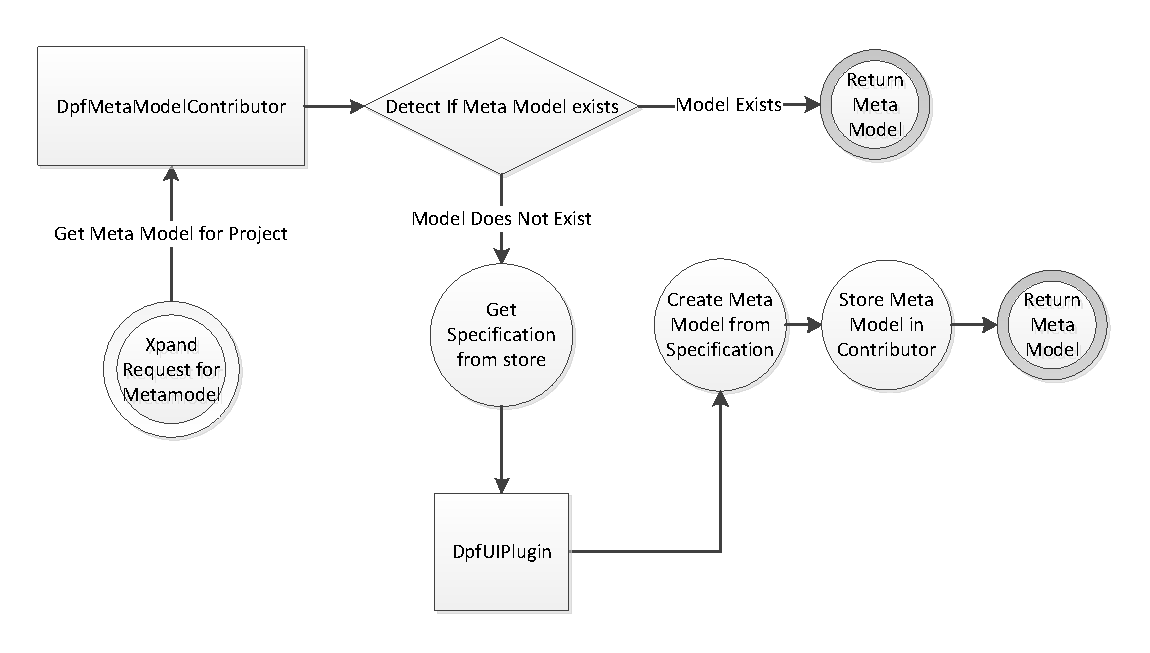
\includegraphics[scale=0.7]{images/metamodel_contributor.pdf}}
  \caption[MetamodelContributor flow chart]{Figure shows the process of retrieving a metamodel for a project.}
  \label{fig:metamodel_contributor_flow}
\end{figure}

Figure~\ref{fig:metamodel_contributor_flow} describes the process of retrieving a metamodel. Xpand will request a metamodel for a project, in which the metamodel contributor will try to look up if it has a metamodel associated with the requested project or not. If not, the metamodel contributor will request that the \codeText{DpfResourceDeltaVisitor} scans the workspace to retrieve any specifications found in either a .prefs file, or a workflow file. The specification found will then be loaded using EMF, and returned to the metamodel contributor where a metamodel object is created with the returned specification as argument. The metamodel contributor then stores the metamodel with the requested project associated for later use and returns the metamodel.

The Eclipse integration and the Xpand generator component both rely heavily on the DPF metamodel. When creating a new DPF Generator Project we specify the location of our DSML through the wizard or the workflow, which then loads the DSML into a metamodel that is associated with the current project. This metamodel is never used for generating code, but only for providing the DSML concepts and its types to the template editor. When generating code, the metamodel and types are instantiated in the workflow, and only exists until the workflow is finished. The template editor's metamodel never has an instance model associated with it, as it is irrelevant.

\subsection{Project Structure}\label{subsec:project_structure}
For the users convenience, we generate a project structure which is ready for use.  Listing~\ref{list:projectstructure} shows the project structure which is generated for the user. The \codeText{src} and \codeText{src-gen} are source code folders where \codeText{src-gen} will contain any generated code. This path is not hardcoded, and can be customized through the workflow file (see listing~\ref{list:workflowexample}). The project is built on top of a Xpand project. This means the project is an Eclipse plug-in which can be used in the same manner as any other Eclipse plug-in project, and we get all the correct dependencies for a Xpand project through the \codeText{MANIFEST.MF} file. The \codeText{.project} file contains details about the project, such as which natures (see next subsection) are activated. This file is essential to let Eclipse know what kind of project we are dealing with. Lastly the \codeText{.settings} folder contains two preference files which are read when the project is recognized as both an Xpand project, and a DPF Generator project. The files define which metamodel is active on the project and where to find the DSML.

\lstset{caption=Listing shows the generated project structure for a DPF Generator Project,label=list:projectstructure,captionpos=b}
\begin{table}[ht]
  \centering
\begin{lstlisting}[showstringspaces=false]
no.hib.dpf.test/
|-- .settings/
|  |-- no.hib.dpf.codegen.xpand.ui.prefs
|  |-- org.eclipse.xtend.shared.ui.prefs                                                                                                                                   
|-- META-INF/
|  |-- MANIFEST.MF
|-- src/
|  |-- template/
|  |   |-- templ.xpt
|  |-- workflow/
|      |-- workflow.mwe
|-- src-gen/
|-- .project
\end{lstlisting}
\end{table}

A template and workflow file are also added. The workflow file contains a simple standard setup, with the DPF Reader component properly defined. The template file contains the "entry" definition of a template, more precisely a \codeText{DEFINE} block for a DPF specification.

\subsection{Project Nature}
In Eclipse the concept of a project nature is to indicate that your project are of a certain type, which uses certain tools. The nature can configure the UI by contributing menu selections, views or any other Eclipse artefact. Natures can also handle project specific properties. 

In the earlier iterations of the codebase, all paths to models was stored in project specific settings. Unfortunately these settings was also workspace specific, which means that if a user checked his project into a VCS and another checked it out, the second user would not have access to the first users settings as to where the models was stored. This problem is avoided by writing a \codeText{.prefs} file in the \codeText{.settings} folder in the project.

This means that the project nature facility in the plug-in is now largely unused, besides always being enabled for new DPF Generator projects. The reason for leaving the code in the plug-in is that it will almost certainly be used in the future if the tool gets further developed.
%   \begin{itemize}
%     \item Plugin and contributor
%     \item Nature?
%     \item Creating project
%     \item Generating project structure with workflow/template <- Illustration
%   \end{itemize}

\section{Shortcomings in the Tool}\label{sec:shortcomings}
\subsubsection{Namespaces and Multiple DSMLs}\label{subsub:namespaces}
In its current state namespaces are not supported. The prefix \codeText{dpf} is hardcoded and used for all types within the metamodel. This poses a problem when one wants to have more than one DSML in the project. It is also not possible to have multiple instance models on one DSML. A solution to this is to run the generator workflow for each DSML and corresponding instance.

This feature was a low priority in this project, and was unfortunately not finished. It might be a usability improvement to manage multiple DSMLs in a single workflow, as well as multiple DSML instances. Multiple DSML instances on a single language requires the implementation of namespaces, as name collisions can occur, and thus returning the wrong node or arrow.

An implementation of this feature is relatively easy. One suggestion is to prefix every entity from the DSML/model with a custom name. Another solution could be to store a map of \codeText{InternalMetamodel}'s and \codeText{InternalModel}'s with the prefix as key.

\subsubsection{Decoupling from \codeText{no.hib.dpf.core}}\label{subsub:decouple}
At this point, there is a very tight coupling between the tool and \codeText{no.hib.dpf.core}. Although a natural dependency, it is problematic that whenever the DPF API is changed, the metamodel might break and its types needs to be updated manually. The nature of the DPF project, where each student works on a separate aspect of the tool, makes it desirable to have each "module" as self sustainable as possible. Learning a new codebase from scratch is a lot of work which can be alleviated by good self-documenting and annotated code, but it is still extra work.

A solution to this problem can be to create an API, beyond the one generated from the DPF Ecore, which is maintained by whoever is responsible for \codeText{no.hib.dpf.core}. Tolvanen and Kelly~\cite{tolvanen:dsm} mentions data-based and message-based APIs to decouple generators from models. A data-based API is basically what we have today, an API which returns parts of the actual model, or a copy. To avoid breaking the API one should mark obsolete methods and classes as \codeText{@Deprecated} rather than removing them. The message-based API is an approach where only proxies for the model are sent back and forth. This means you operate on proxy objects that resolves to a primitive like string or integer at its most basic form.

\subsubsection{Test Coverage}
The current test coverage of the tool is poor. The metamodel and type classes are the only components which have some tests written. The coverage for these components are very limited as well. Besides the lack of time, the issue addressed in section \ref{subsec:mm_test} is the main reason for not creating more tests for the metamodel itself. Other components like the workflow reader and UI related code can be tested programmatically.

\subsubsection{Implementing Constraints and Predicates Using Types}\label{subsub:shortcoming_constr}
When this tool was developed, the signature file (see section~\ref{sec:dpf}) was hardcoded along with its predicates. It was not a priority to do anything about these types, as the Ecore helper within our metamodel exposed the needed functionality. The latest version of DPF Editor gives the opportunity to define custom predicates which opens up new possibilities. There was unfortunately no time to implement this.

Chapter~\ref{chap:case_study} will present a way to simplify the handling of constraints using extensions.

\section{Feature Overview}
We wrap up with an overview of what has been achieved through the development in this project:
\begin{description}
  \item[Xpand metamodel] \hfill \\
  The Xpand metamodel for DPF is the core functionality that lies at the heart of what has been developed in this project. The metamodel is a mapping from the DPF model types to our custom Xpand types. The types exists only in the metamodel, and is available through queries.
  \item[Type system] \hfill \\
  We have defined a type system which Xpand can understand for each of the modelling constructs in DPF. This enables us to easily define new functionality for each modelling constructs, such as DSML specific getters and setters, or utilizing the functionality already defined in the DPF Ecore metamodel.
  \item[Workflow integration] \hfill \\
  With the implementation of the DPF Reader component, we have integrated the metamodel with the Modeling Workflow Engine (MWE). This results in a seamless use of the metamodel between the different components that Xpand offers.
  \item[Eclipse integration] \hfill \\
  With the implementation of a \emph{metamodel contributor}, we can take advantage of all the features which Xpand has to offer. We get editor support for template editing with Xpand, extension editing with Xtend and constraints checking with Check. The editor support contains code completion, syntax coloring, error highlighting, source navigation and refactoring. 
  \item[Project environment] \hfill \\
  As part of the Eclipse integration, we have implemented a project environment that defines a wizard for generating a project structure suitable for code generation. There is also a facilitated a \emph{project nature}.
\end{description}

The time invested in creating this functionality is time well spent, as using any of the alternative approaches (section~\ref{subsec:considered_approaches}) would have been an inferior solution technologically.

Lastly, let us take a look at our problem description in section~\ref{sec:problem_description}. We stated that an ideal solution would solve a few requirements:
\begin{description}
  \item[Clear expression of domain concepts] \hfill \\
  Through the interpreted nature of Xpand, we are able to create an environment for code generation based on the concepts of a DSML rather than an instance model.
  \item[Integration with Eclipse] \hfill \\
  The metamodel and the metamodel contributor give us access to all the features Xpand has to offer.
  \item[Standalone generator] \hfill \\
  This requirement is the one which is not completely fulfilled. A framework with the size of Xpand is bound to have some dependencies. The bright side is that a generator can be executed without Eclipse, with only Xpand, log4j and \codeText{no.hib.dpf.core} as dependencies.
\end{description}
  





\chapter{Demonstrating the Tool}\label{chap:case_study}
This chapter will demonstrate how to use the Xpand framework together with the DPF metamodel and its Eclipse integration. We will generate code for the Play~\cite{playframework} web framework based on a simple DSML. Generating code for a web framework is an excellent use case, because of the similar traits from one application to another. 
% If one defines two web applications in the same framework, they will most likely share the same structure. This makes web applications a popular domain for MDE and code generation~\cite{Vis08}~\cite{uwe4jsf}. 

\section{Components/Packages}
\begin{description}
  \item[\codeText{no.hib.dpf.codegen.examples.dpfplay}] \hfill \\
  Contains the generator implementation.
  \item[\codeText{no.hib.dpf.codegen.examples.dpfplay.ui}] \hfill \\
  This plug-in contains the Eclipse integration for the generator.
\end{description}

The component name chosen is \codeText{codegen} like the DPF Xpand metamodel. The sub component is called examples, as a common subcomponent for all code generation related example projects. The name chosen for the project is "dpfplay".
\begin{quote}
  \emph{NOTE: The plug-ins are part of the reference example project. This chapter will not explain the Eclipse integration found in the \codeText{no.hib.dpf.codegen.examples.dpfplay.ui} plug-in.}
\end{quote}

\section{Choosing a Framework}
The following is a short evaluation of the candidates chosen for this tool demonstration. The criterias used was simple;
a modern framework with as little configuration and boilerplate\footnote{Boilerplate code is a term for code which appears in many places with little to none alterations.} code as possible.  Most popular frameworks today is based on the \emph{Model View Controller (MVC)} pattern, which give them similar properties. If one defines two web applications in the same framework, they will most likely share the same structure. This makes web applications a popular domain for MDE and code generation~\cite{Vis08}~\cite{uwe4jsf}. 

The model part of an MVC framework is usually the most generic and simple to generate code for. \emph{Controllers} and \emph{View} vary a lot more in how they function.  

After a short evaluation the Play Framework was chosen. In addition to fitting the criterias, it is made for Java (and Scala) which was ideal considering the time left in the project. As we will discover, Play enables us to get results with very little code.

\subsection{Lift}
Lift~\cite{liftweb} is a web framework based on the Scala programming language, which focuses on security, scalability and ease of use. The framework tries to fill the same need as other web frameworks such as Ruby-on-Rails and Spring, but tries to improve on the shortcomings other frameworks exhibits. Lift follows the MVC pattern to enforce separation of concern; unlike JSP, Lift does not allow code in the templates. The framework also benefits from Scala's Actor model which provides concurrency in a safe and robust manner. 

\subsection{Django}
Django~\cite{django} is another web framework based on the MVC paradigm which uses the Python programming language. Its focus is to hide the boilerplate code and focus on the functionality. 
Among the wide range of features you find Object-Relational Mapping (ORM), caching framework, template engine, a standalone web-server and automatically generated CRUD interface for your model classes. 

\subsection{Grails}
Grails~\cite{grails} uses the Groovy programming language which is a dynamic language running on the JVM. As with Django and Lift, Grails uses
the MVC pattern. Under the hood it uses a lot of the functionality inside Spring, but stays clear of any XML configuration.

\subsection{Play Framework}
The Play Framework~\cite{playframework} is a MVC web framework for Java and Scala. It aims to be a more effective alternative to other Java frameworks like Spring and Java EE. Play comes with its own runtime that loads code changes directly into the JVM, and removes the need to restart the application server each time a change is made. Another notable feature is the template engine, which uses Groovy as expression language. The result is a concise syntax with less boilerplate code.

\section{Problem Description}
Creating a working example for the code generation tool is needed to demonstrate how it works. The process of creating a generator project is simple, yet it demands some hand coding to create the templates, which are the most important part. Any UI integration of the generator will need to be hand coded in the same manner as any other Eclipse plug-in.

Through this chapter we will demonstrate a simple code generator, which generates simple Java model classes for the Play framework using a simple DSML. We will utilize Play's built-in modules to provide a CRUD (Create, Read, Update, Delete) interface using our generated classes. 

This chapter acts as a tutorial on how to use the code generation tool. The code for this example project can be found at \url{http://dpf.hib.no/downloads/}. It contains a more elaborate example with Eclipse integration for the generator. 

This example project was developed using Eclipse Indigo (modelling tools bundle) with Xpand and the DPF Xpand metamodel installed. The version of Play framework used is 1.2.4.

% The project contains some UI integration with Eclipse so that we get a sense on how to integrate the generator as part of the UI workflow, and not running the workflow file directly through the Modeling Workflow Engine (MWE, see~\ref{subsub:workflow}). The tool will use DSML which is hard coded as the typing of an editor. This editor can create model classes for Play! based on the hard coded typing. Generating code happens through user interaction, where the instance model gets passed to the generator for processing.

\section{Creating the Generator}
\subsection{What to Generate}
As stated in the previous section, we want to generate simple model classes for a Play project. The example is very simple, and will not entail the generation of any behaviour oriented code. We will handle multiplicity constraints to give an example on how to use them in their current state. In section~\ref{sec:create_generator} we briefly discuss the creation of a code generator and what is needed for creating one; mainly a sample input and output to clearly define the generator's requirements. The templates in the generator can be regarded as transformation rules, and it is thus necessary to see what you want to transform and what it should result in.

The first thing we need to do is define a DSML for our problem. This step is not necessarily a part of the code generation activity, as the language might be pre-defined.
% \newpage

\begin{figure}[h]
  \centering
  \centerline{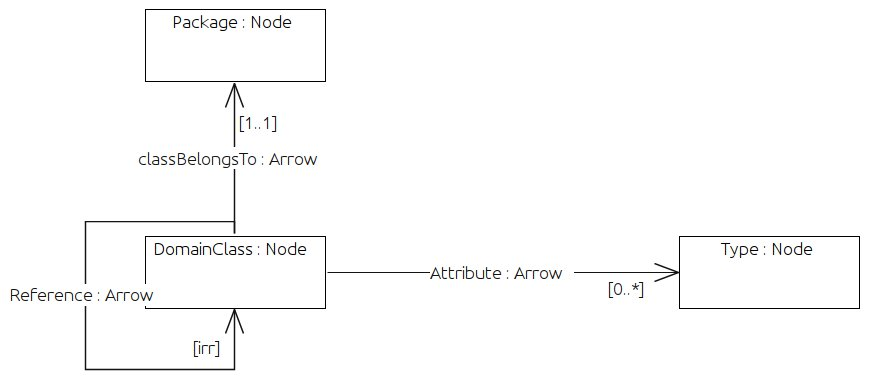
\includegraphics[scale=0.5]{images/web_dsml.jpeg}}
  \caption[DSML for dpfplay]{Figure depicts a simple DSML for creating domain classes.}
  \label{fig:web_dsml}
\end{figure}

Lets go through the DSML step by step:
\begin{enumerate}
  \item We define three \codeText{Nodes} which have the type names \codeText{DomainClass}, \codeText{Type} and \codeText{Package}.
  \item A \codeText{DomainClass} may have a \emph{reference} to one or more \codeText{DomainClasses}.
  \item A \codeText{DomainClass} can not reference itself. This is enforced by the irreflexive \codeText{[irr]} constraint.
  \item A \codeText{DomainClass} has exactly one \codeText{Package} (\codeText{[1..1]} multiplicity constraint).
  \item A \codeText{DomainClass} can have zero or more \codeText{Types} associated.
\end{enumerate}

In short, this DSML enables us to create \codeText{DomainClass} nodes that belongs to a \codeText{Package}. The \codeText{DomainClass} may or may not have any attributes or other \codeText{DomainClasses} associated with it.

To properly understand how to create our generator, we need to create a sample input model:
\begin{figure}[h]
  \centering
  \centerline{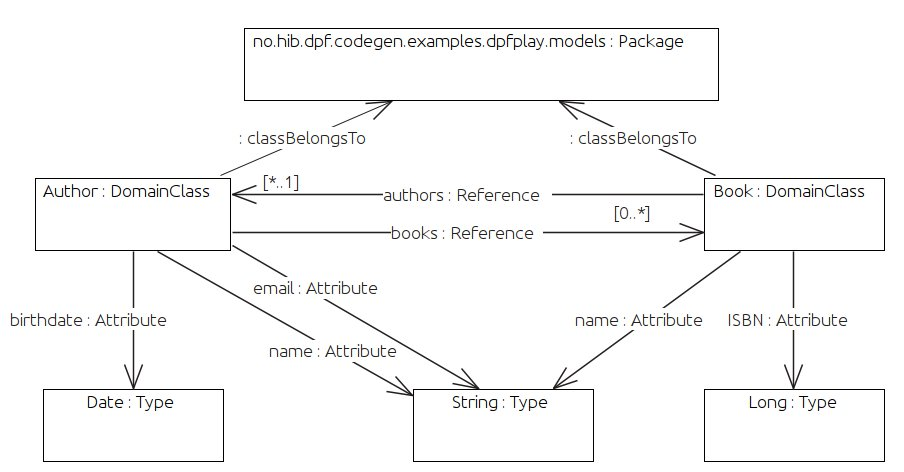
\includegraphics[scale=0.5]{images/dsml_instance.jpeg}}
  \caption[Sample instance model for dpfplay]{An instance model for the DSML (\ref{fig:web_dsml}).}
  \label{fig:web_instance}
\end{figure}

The instance model in figure~\ref{fig:web_instance} shows an example with nodes \codeText{Author} and \codeText{Book} which both are typed by \codeText{DomainClass}. Each node has a few attributes shown by the arrows typed by \codeText{Attribute}. There are also a zero-to-many relation between \codeText{Author} and \codeText{Book} (an author can have zero or more books), as well as a one-to-many relation from \codeText{Book} to \codeText{Author} (one book can have many authors).

Now that we have a sample input defined, we can define what we want to achieve with the generator. This example will create very simple model classes which forms the foundation in a Play web application. 

\lstset{language=Java,caption=Listing shows a preliminary draft of the code we want to generate.,label=list:gencode,captionpos=b}
\begin{table}[hp]
  \centering
\begin{lstlisting}[showstringspaces=false]
Author.java

package no.hib.dpf.codegen.examples.dpfplay.model;

import java.util.Date;
import java.util.ArrayList;

public class Author {
  public String name;
  public String email;
  public Date birthdate;
  public ArrayList<Book> books;

  public Author(String name, String email, Date birthdate, ArrayList<Book> books) {
    this.name = name;
    this.email = email;
    this.birthdate = birthdate;
    this.books = books;
  }
}

Book.java

package no.hib.dpf.codegen.examples.dpfplay.model;

import java.util.ArrayList;

public class Book {
  public String name;
  public String isbn;
  public ArrayList<Author> authors;

  public Book(String name, String email, ArrayList<Author> authors) {
    this.name = name;
    this.isbn = isbn;
    this.authors = authors;
  }
}
\end{lstlisting}
\end{table}

Listing~\ref{list:gencode} shows a draft of how we would like the code to look after code generation. The seasoned reader might see that we have defined our data fields as \emph{public}, rather than \emph{private}. This is an example of the convenience Play provides through its own runtime; all public fields will have getters and setters generated. Model classes in Play will typically also contain Java Persistence API (JPA) annotations for the persistence of the models. These will be added at a later point.

Now that we have defined our DSML, instance model and output sample, we can start thinking about creating a generator project and define our templates.

\subsection{Creating a Generator Project}
When selecting the \emph{New} wizard in Eclipse, we find a new entry under the DPF category, \emph{DPF Generator Project}. This is part of the functionality we defined in the \codeText{no.hib.dpf.codegen.xpand.ui} plug-in.

\begin{itemize}
  \item \emph{Select DPF Generator Project as figure~\ref{fig:codegen_wizard1} shows.}
\end{itemize}

\begin{figure}[h]
  \centering
  \centerline{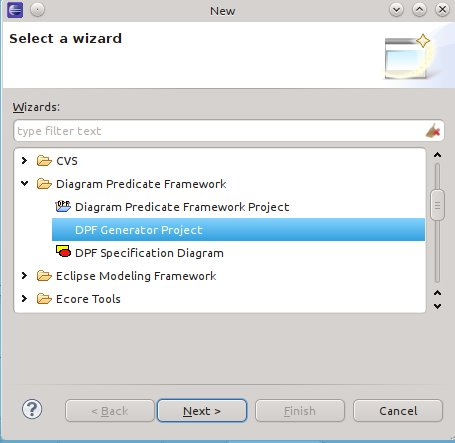
\includegraphics[scale=0.53]{images/codegen_wizard1.jpeg}}
  \caption[Eclipse wizard]{Eclipse \emph{new} wizard showing the DPF category with DPF Generator Project.}
  \label{fig:codegen_wizard1}
\end{figure}

Figure~\ref{fig:codegen_wizard2} shows the DPF Generator Wizard. As shown, there are two fields in the wizard. The project name is obligatory while the location of the DSML is optional. As discussed in section~\ref{subsec:editor_support}, the DSML is needed to enable the editor support. Even though a DSML is not defined for the project you create, one can define the location where it is supposed to be. The DSML will then load upon creation. One can also use the location of DSMLs in other projects in the workspace. We will leave the metamodel location blank for now, as we wish specify it later.

\begin{figure}[h!]
  \centering
  \centerline{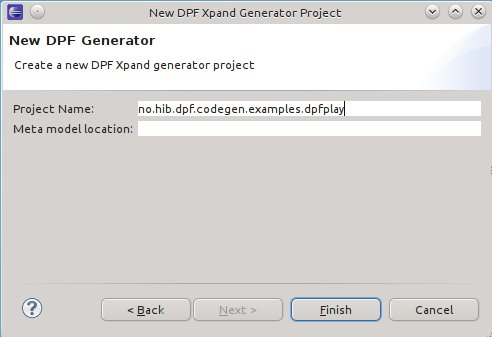
\includegraphics[scale=0.7]{images/codegen_wizard2.jpeg}}
  \caption[DPF Generator wizard]{Figure shows the DPF Generator Wizard.}
  \label{fig:codegen_wizard2}
\end{figure}

\begin{itemize}
  \item \emph{Set project name to \codeText{no.hib.dpf.codegen.examples.dpfplay}}.
  \item \emph{Leave metamodel location blank and press "Finish"}.
\end{itemize}

We have now a ready to use project structure (see~\ref{subsec:project_structure}). As the DSML location has not been defined, the generated template stub will show an error as the \codeText{dpf} namespace is not found.

Before proceeding, we want to define the DSML and instance model using the DPF Editor, so that we can get editor support in the later steps.

\begin{itemize}
  \item \emph{Create a new folder \textbf{models} in our project.}
  \item \emph{Inside the \textbf{models} folder, create a new DPF specification with the name "metamodel".}
%   \item \emph{The \textbf{models} folder should now contain a "metamodel.dpf" and a "metamodel.dpf.xmi".}
  \item \emph{Open the specification and define the DSML in figure~\ref{fig:web_dsml}.}
  \item \emph{Create another DPF specification with the name "author" within the \textbf{model} folder. Use "metamodel.dpf.xmi" as the typing for the specification.}
  \item \emph{Open the specifcation and define it using our model from figure~\ref{fig:web_instance}.}
\end{itemize}

\subsection{Defining the Workflow}
With the project structure a workflow is generated, it contains almost everything that is needed to run it. The generated workflow should look like so:

\lstset{language=XML,caption=The generated workflow file in a DPF Generator Project,label=list:codegenworkflow,captionpos=b}
\begin{table}[h]
  \centering  
  \begin{lstlisting}[showstringspaces=false]
<?xml version="1.0" encoding="UTF-8" standalone="no"?>
<workflow>
  <!-- workflow properties -->
  <property name="dpf_model" value=""/>
  <property name="dpf_metamodel" value=""/>

  <property name="src-gen" value="src-gen"/>

  <!-- set up EMF, only needed when using URI's -->	
  <bean class="org.eclipse.emf.mwe.utils.StandaloneSetup">
      <platformUri value=".."/>
  </bean>
	
  <!-- instantiate metamodel-->
  <bean class="no.hib.dpf.codegen.xpand.metamodel.DpfMetamodel" id="mm_dpf"/>
	
  <!-- DPF component -->
  <component class="no.hib.dpf.codegen.xpand.metamodel.workflow.DpfReader">
      <dpfMetaModel value="${dpf_metamodel}"/>
      <dpfModel value="${dpf_model}"/>
      <metaModel idRef="mm_dpf"/>
      <modelSlot value="dpf"/>
  </component>
	
  <!--  generate code -->
  <component class="org.eclipse.xpand2.Generator">
      <metaModel idRef="mm_dpf"/>
      <expand value="template::templ::main FOR dpf"/>
      <outlet path="${src-gen}">
	  <postprocessor class="org.eclipse.xpand2.output.JavaBeautifier"/>
      </outlet>
  </component>
</workflow>
  \end{lstlisting}
\end{table}

\newpage

As listing~\ref{list:codegenworkflow} shows, we get a workflow file with the DPF Reader component inserted (see~\ref{subsub:workflow} for an explanation of a workflow). The only attributes which must be set is the location for a DSML and an instance model.

\begin{itemize}
  \item \emph{Insert the DSML's path \codeText{models/metamodel.dpf.xmi} into the\newline \codeText{dpf\_metamodel} property's value attribute.}
  \item \emph{Insert the instance model's path \codeText{models/author.dpf.xmi} into the\newline \codeText{dpf\_model} property's value attribute.}
  \item \emph{Save the file.}
\end{itemize}
Defining the instance model at this moment, does not affect anything as it is only used when running the generator. The definition of the DSML on the other hand is more interesting; every time a resource gets changed in the project, we scan it and try to retrieve a valid path to a DSML. The first check is to see if a workflow file is defined. If so, it will look for the \codeText{dpf\_metamodel} attribute and see if a value is defined. If a value is defined, it will mirror the path in the \emph{no.hib.dpf.codegen.xpand.ui.prefs} file and load the specifcation for use in the DPF Xpand metamodel. If no such value is found in the attribute, the tool will try to find a path in the \emph{no.hib.dpf.codegen.xpand.ui.prefs} file. If this fails as well, no metamodel will be loaded for the project. This solution is admittely not the most optimal, as it will not work with more than one DSML per project (in its current state).

\subsection{Defining the Template}
Now that we have defined a DSML in the workflow file, we get editor support. We have defined our input model as well, and created a draft of our output. We will now define a template for creating model classes and use Xtend and Java extensions where it is needed.

\begin{quote}
  \emph{NOTE: When creating/reading templates in Xpand, make sure that the font encoding is set to UTF-8 or another encoding which support \emph{guillemets} (« and »).}
\end{quote}

\subsubsection{Basic Xpand Concepts}
\begin{itemize}
  \item \emph{Open the templ.xpt file.}
\end{itemize}
\flushleft The only content of the file is:
% \lstset{title=,caption=} %DO NOT CHANGE OR SET LIST CAPTION BEHIND THIS WITHOUT RESETTING
\begin{plainlisting}
«IMPORT dpf»

«DEFINE main FOR dpf::Specification»

«ENDDEFINE»
\end{plainlisting}{}
A \codeText{DEFINE} block for a \codeText{Specification} type is required to start with, as it is the assumed input object for the generator. \codeText{DEFINE} statements are also called \emph{definitions} or \emph{templates}. The \codeText{DEFINE} statements are the building blocks of the template files; each statement can invoke other \codeText{DEFINE} statements and so on. 

In our example template, the \codeText{main} block engulfs all of the other \codeText{DEFINE} blocks. The \codeText{main} block is invoked through the workflow engine using \codeText{<expand~value="template::templ::main~FOR dpf"/>}. \codeText{dpf} is the \emph{model slot} defined in the DPF Reader (see~\ref{subsec:reader_workflow}). The \codeText{Specification} object that represents a DPF model has a hierarchy which is reflected in the templates we create. 

The next step in our template is to create a \codeText{DEFINE} statement for a graph.
\begin{quote}
  \emph{NOTE: Guillemets are created using \emph{Ctrl+<} for « and \emph{Ctrl+Shift+<} for ».}
\end{quote}
\begin{itemize}
  \item \emph{Add the following listing to templ.xpt:}
  \begin{plainlisting}
«DEFINE graph FOR dpf::Graph»

«ENDDEFINE»
  \end{plainlisting}
\end{itemize}
To invoke the \codeText{graph} block from \codeText{main}, we need an \codeText{EXPAND} statement. The \codeText{EXPAND} statement is used for invoking other \codeText{DEFINE} blocks.
\begin{itemize}
  \item \emph{Inside the \codeText{main} block, add:}
  \begin{plainlisting}
«EXPAND graph FOR this.graph»
  \end{plainlisting}
\end{itemize}
The \codeText{EXPAND} statement expands the \codeText{graph} block with the \codeText{Specification} object's internal \codeText{graph} object. The \codeText{this} handle refers to the object which the \codeText{DEFINE} block pertains to. 

Our DSML defines the concept \codeText{DomainClass} which represents a model class for use in a Play web application. The next step in our template is to iterate over every \codeText{DomainClass} which is defined in the instance model.
\begin{itemize}
  \item \emph{Create a new \codeText{DEFINE} statement:}
  \begin{plainlisting}
«DEFINE domainclasses FOR dpf::DomainClass»

«ENDDEFINE»
  \end{plainlisting}
  \item \emph{Add the following line to the \codeText{graph} \codeText{DEFINE} block:}
  \begin{plainlisting}
«EXPAND domainclasses FOREACH this.getDomainClasses()»
  \end{plainlisting}
\end{itemize}
We start to see how the DPF Xpand metamodel lets us express the concepts of our DSML rather than the DPF Ecore model (see section~\ref{sec:problem_description} for an example). The \codeText{getDomainClasses()} method is a custom convenience method defined in the DPF Xpand metamodel's \codeText{GraphType}. Using this method we iterate over every \codeText{DomainClass} instead of its type node, \codeText{Node}. An important observation is that we use \codeText{FOREACH} when we want to invoke a \codeText{DEFINE} statement for each element in a collection.

In Java, a class is defined in its own file. This means we need to create a Java class file for each \codeText{DomainClass} type in our instance model. This is achieved using the \codeText{FILE} statement.
\begin{itemize}
  \item \emph{Inside the \codeText{domainclasses} block, add:}
\lstset{label=list:gencode,captionpos=b}
  \begin{plainlisting}
«FILE this.name.toFirstUpper() + ".java"»
«ENDFILE»
  \end{plainlisting}
\end{itemize}
The \codeText{FILE} statement creates a file with a name as argument. The example shows that we retrieve the \codeText{name} of the current \codeText{DomainClass} using \codeText{this}. We also take advantage of the built-in string operation \codeText{toFirstUpper()} that returns the name with the first letter as uppercase.

\begin{itemize}
  \item \emph{Run the MWE workflow by right-clicking the workflow file and selecting "Run As -> MWE Workflow".}
\end{itemize}
We should now see two empty files called "Author.java" and "Book.java" in our \codeText{src-gen} folder.

The basic constructs of Xpand are now familiar and we can start defining the content of the files we generate. From within the \codeText{FILE} block we can insert the first statements.

\subsubsection{Creating an Extension}
\begin{itemize}
  \item \emph{Inside the \codeText{FILE} block, add:}
  \begin{plainlisting}
package «this.getAClassBelongsTos().get(0).target.name»;
  \end{plainlisting}
  \item \emph{Run the workflow.}
\end{itemize}
When executing the workflow, we generate two files which only contains a package declaration in the \codeText{src-gen} folder. Although the statement looks a bit messy, the semantics are easy to grasp. From the current \codeText{DomainClass} type, we retrieve all the outgoing \codeText{classBelongsTo} arrows. The DPF Xpand metamodel defines every getter for an outgoing arrow as a collection for consistency reasons throughout the tool, despite the use of a \codeText{[1..1]} multiplicity constraint on the particular arrow. When we have retrieved the arrow, we call the target attribute, which retrieves the node that the arrow points to, and lastly we fetch the target node's name. We observe that Eclipse displays an error icon on our generated files, and tells us that the files are in the wrong package. This happens because we have told the generator to output everything to the \codeText{src-gen} directory. In our metamodel we have specified that each model class can have its own package which means we do not want to hardcode the package path. Fortunately we can delimit the \codeText{FILE} statement's name argument with a slash, thus defining the output file's path.

Creating a valid path for the \codeText{FILE} statement is an example on where you can use extensions, rather than perform program logic within the template. Replacing all "." with a "/" is done using a single line of code, but it will look tidier with a descriptive method name.
\begin{itemize}
  \item \emph{Create a new package called \codeText{extensions}.}
  \item \emph{Create a new file in the \codeText{extensions} package called \textbf{dpfplay.ext}.}
  \item \emph{Insert the following code:}
  \begin{plainlisting}
import dpf;
getPackage(DomainClass d):
    d.getAClassBelongsTos().get(0).target.name.replaceAll("\\.", "/") + "/";
  \end{plainlisting}
  \item \emph{Insert the following right below the \codeText{import dpf} statement in our template:}
  \begin{plainlisting}
«EXTENSION extensions::dpfplay»
  \end{plainlisting}
  \item \emph{Modify the \codeText{FILE} statement inside the \codeText{domainclasses} block:}
  \begin{plainlisting}
«FILE packageName(this)+this.name.toFirstUpper() + ".java"»
  \end{plainlisting}
  \item \emph{Run the workflow again.}
\end{itemize}
The generator should now output the files into its proper package \codeText{no.hib.dpf.codegen.examples.dpfplay.models}.

The \codeText{Type} nodes in our model can be any type as we have not intended any restrictions on which types that are allowed. We must then take care of this inside our templates (or extensions).
\begin{itemize}
  \item \emph{Create a new \codeText{DEFINITION} statement called imports:}
  \begin{plainlisting}
«DEFINE imports FOR List[dpf::Attribute]»
    «FOREACH this AS e»
	«IF e.target.name == "Date"»
	    import java.util.Date;
	«ENDIF»
    «ENDFOREACH»
«ENDDEFINE»
  \end{plainlisting}
  \item \emph{Add an \codeText{EXPAND} statement below the package definition in \codeText{domainclasses}:}
  \begin{plainlisting}
«EXPAND imports FOR this.getAAttributes()»
  \end{plainlisting}
\end{itemize}
We now have an import for the \codeText{Date} type if it is defined in the template. In a more advanced scenario, it would perhaps be easier to use a fully qualified name for the import to avoid long chains of \codeText{IF} statements for definition of every possible type. Clearly defining which types are allowed would also be a way to fend off unnecessary complexity.
% A robust generator should be able to handle situations where the input is unexpected

\subsubsection{Creating a Java Extension}
Creating collections of \codeText{Reference} types is possible, and this means we need to handle this in a proper manner. We need to figure out if the \codeText{Reference} is constrained with a multiplicity constraint, and what the bounds are. 

In the DPF Ecore metamodel, constraints are defined on the \emph{graph} and not on the nodes and arrows it constrains\footnotemark. Each constraint contains a list of the nodes and arrows it constrains, and a reference to the predicate which it is an instance of. To identify what kind of constraint we are dealing with, we need to look at its predicate. When writing templates, these are the idiosyncrasies which can be dealt with through defining operations in our DPF Xpand metamodel's type system. Unfortunately there is no solution for this in place for various reasons (see section~\ref{subsec:type_system}). Creating an extension to simplify the process is a satisfactory solution for now.

In Xpand we can define Java extensions which are an Xtend function that calls methods in external Java classes.

\footnotetext{In the latest version of the DPF core, constraints can be retrieved on the nodes and arrows it constrains. The code generation tool is not (yet) compatible with the new API.}

\begin{itemize}
  \item \emph{Create a new Java file in the \codeText{extensions} package called \textbf{TemplateHelper.java}.}
  \item \emph{Insert the following content:}
  \begin{plainlisting}
package extensions;

import no.hib.dpf.core.Node;

public class TemplateHelper {
    public static String printArrayImport(Node n) {
	return "import java.util.ArrayList;"; 
    }
}
  \end{plainlisting}
  \newpage
  \item \emph{Insert into \textbf{dpfplay.ext}:}
  \begin{plainlisting}
String publicArrayImport(DomainClass d):
    JAVA extensions.TemplateHelper.printArrayImport(no.hib.dpf.core.Node); 
  \end{plainlisting}
  \item \emph{Insert a call to this extension in your template below the \codeText{imports EXPAND} statement.}
\end{itemize}
For now we hardcode the return value from the Java extension. 

Type inference in Xtend\footnote{Xtend is the Xpand extension language, see section~\ref{sec:xpand}.} does not apply to Java extensions which is why we have specified String as the return value. One must also use the fully qualified name of the class and method to invoke it.

\subsubsection{Finishing the Template}
Up until now we have been thorough with the explanations of the Xpand language and its concepts. We are now equipped with enough knowledge to speed things up.

\begin{itemize}
  \item \emph{Below the \codeText{printArrayImport} insert:}
  \begin{plainlisting}
public class «this.name.toFirstUpper()» {                                                                             
    «getDomainClassAttrRef(this.getAAttributes(), this.getAReferences())»                                                                                                                                                                 
                           
    public «this.name»(«paramList(this.getAAttributes(), this.getAReferences())») {                                             
	«constructorSetAttributes(this.getAAttributes(), this.getAReferences())»                                            
    }   
}        
  \end{plainlisting}
  \item \emph{The extensions above are found listed below.}
\end{itemize}

All of the defined extensions needs to know if we have a multiplicity constraint so that it can write \codeText{ArrayList<Book>} instead of \codeText{Book}. The extensions shown in listing~\ref{list:xtendextension} shows both Xtend extensions as well as Java extensions. The listing below demonstrates the vast amount of code needed to handle simple constraints using the DPF API directly.
\newpage
% \lstset{language=Java,caption=Listing shows the Java extension file for resolving multiplicity constraints.,label=list:javaextension,captionpos=b}
% \begin{table}[h!]
%   \centering   
%  \begin{lstlisting}[showstringspaces=false]
\begin{plainlisting}
package extensions;
import java.util.List;
import no.hib.dpf.core.Arrow;
import no.hib.dpf.core.Constraint;
import no.hib.dpf.core.Node;

public class TemplateHelper {
    public enum Mult {MANY_TO_ONE, ONE_TO_MANY, MANY_TO_MANY, ONE_TO_ONE};
    private static String MULT_CONSTRAINT = "[mult(m,n)]";
    public static Mult parseConstraint(String expr) {
        String f,l;
        Mult m;
        try {
            f = expr.substring(0, expr.indexOf(','));
            l = expr.substring(expr.indexOf(',') + 1, expr.length());
            
            if(Integer.parseInt(f) == 1 && Integer.parseInt(l) == -1) {
                m = Mult.ONE_TO_MANY;
            } else if(Integer.parseInt(f) == -1 && Integer.parseInt(l) == -1) {
                m = Mult.MANY_TO_MANY;
            } else if(Integer.parseInt(f) == -1 && Integer.parseInt(l) == 1) {
                m = Mult.MANY_TO_ONE;
            } else m = Mult.ONE_TO_ONE;
        } catch (StringIndexOutOfBoundsException e) {
            m = Mult.ONE_TO_ONE;
        }
        return m;
    }
    public static String printArrayImport(Node n) {
        List<Arrow> la = n.getOutgoingArrows();
        boolean ret = false;
        for(Arrow a : la) {
            ret = hasOneOrManyToOtherConstraint(a);
            if (ret) return "import java.util.ArrayList;"; 
        }
        return "";
    }
    public static String getAttr(Arrow a) {
        if(hasOneOrManyToOtherConstraint(a)) return "private ArrayList<" +
                    a.getSource().getName() + "> " + a.getName() + ";";
        else return "public " + a.getTarget().getName() + " " + a.getName() + ";";
    }
\end{plainlisting}
\newpage
\begin{plainlisting}
    public static boolean hasOneOrManyToOtherConstraint(Arrow a) {
        for(Constraint c : a.getGraph().getConstraints()) {
            if(c.getPredicate().getSymbol() != null &&
                    c.getPredicate().getSymbol().equals(MULT_CONSTRAINT)) {
                for(Arrow tmp : c.getConstrainedArrows()) {
                    if(tmp != null && a != null && tmp.getId() == a.getId()
                            && !parseConstraint(c.getParameters()).equals(Mult.MANY_TO_ONE)) {
                        return true;
                    }
                }
            }
        }
        return false;
    }

    public static String getParamList(List<Arrow> aa, List<Arrow> aaa) {
        StringBuffer ret = new StringBuffer();
        ret.append(paramList(aa));
        if (aaa.size() != 0 && ret.length() != 0) 
            ret.append(", " + paramList(aaa));
        return ret.toString();
    }
    private static String paramList(List<Arrow> aa) {
        StringBuffer ret = new StringBuffer();
        for(int i = 0; i < aa.size(); ++i) {
            Arrow a = aa.get(i);
            if(hasOneOrManyToOtherConstraint(a)) ret.append("ArrayList<" +
                    a.getSource().getName() + "> " + a.getName());
            else ret.append(a.getTarget().getName() + " " + a.getName());
            if(i < aa.size()-1) ret.append(", ");
        }
        return ret.toString();
    }
    public static String getConstructorInit(List<Arrow> aa, List<Arrow> aaa) {
        StringBuffer ret = new StringBuffer();
        for(int i = 0; i < aa.size(); ++i) {
            Arrow a = aa.get(i);
            ret.append("this." + a.getName() + " = " + a.getName() + ";"); 
        }
        return ret.toString();
    }
}
\end{plainlisting}
%   \end{lstlisting}
% \newpage
% \end{table}

\lstset{caption=Listing shows the Xtend extensions for our generator.,label=list:xtendextension,captionpos=b,breaklines=true}
\begin{table}[h!]
  \centering  
  \begin{lstlisting}[showstringspaces=false]
import dpf;
extension org::eclipse::xtend::util::stdlib::io;
packageName(DomainClass d):
    d.getAClassBelongsTos().get(0).target.name.replaceAll("\\.", "/") + "/";
    
String printArrayImport(DomainClass d):
    JAVA extensions.TemplateHelper.printArrayImport(no.hib.dpf.core.Node);

getDomainClassAttrRef(List[dpf::Attribute] attr, List[dpf::Reference] ref):
    let attrRet = attr.collect(e|getAttr(e)) :
        attrRet.addAll(ref.collect(e|getRef(e)));
        
String getAttr(dpf::Attribute a):
    JAVA extensions.TemplateHelper.getAttr(no.hib.dpf.core.Arrow);
String getRef(dpf::Reference r):
    JAVA extensions.TemplateHelper.getAttr(no.hib.dpf.core.Arrow);
    
String paramList(List[dpf::Attribute] attr, List[dpf::Reference] ref):
    JAVA extensions.TemplateHelper.getParamList(java.util.List, java.util.List);
    
constructorSetAttributes(List[dpf::Attribute] attr, List[dpf::Reference] ref):
    let constructorInitList = attr.collect(e|"this." + e.name + " = " + e.name + ";") :
        constructorInitList.addAll(ref.collect(e|"this." + e.name + " = " + e.name + ";"));
  \end{lstlisting}
\end{table}
Using Java extensions to mitigate the unpractical DPF API results in verbose code which we would like to avoid. The solution entails looping through all the constraints defined for the graph, finding the ones which are instances of the multiplicity predicate, and then looping through its constrained arrows comparing each one against the outgoing reference arrows of our \codeText{DomainClass} node. This can be achieved in a slightly more consise and elegant way using the Xtend language.

When we run the workflow, Xpand should generate two Java classes which contains valid code. The classes demonstrate handling multiplicity by checking if each reference is constrained by a multiplicity constraint. The example code is very simple and uninteresting, but has potential to define a lot more with few adjustments.

To make the example a little bit more interesting, we will generate a CRUD (create,read, update, delete) interface for our model classes. Fortunately Play makes this very easy for us with its built-in CRUD module.
% \subsection{Creating UI integration}

\section{Creating a Play Project}
The Play framework comes with a plug-in for Eclipse. The functionality is limited due to the separate runtime that is provided with the framework. The Play runtime comes with a web server for testing the web application. Everytime a resource is changed and saved, the Play runtime will update the application on the fly. Creating a new Play project is achieved through the Play runtime's command-line interface (CLI). This tool creates and administers the projects. It controls which modules that should be active, running tests and it generates IDE specific configuration files for each project.

The first step is to obtain the Play framework from the project's web site. The version used in this example is 1.2.4, and not the most recent version. Version 2 was recently released with a lot of improvements. Unfortunately this release was too late for the use in this thesis.

\begin{enumerate}
  \item Obtain Play from \url{http://www.playframework.org/documentation/1.2.4/install}. Follow installation instructions.
  \item Create new project using \codeText{play new dpfcrud}.
  \item Create Eclipse-project configuration with \codeText{play eclipsify dpfcrud}.
  \item Import project into Eclipse workspace using the import wizard.
\end{enumerate}

\subsection{Configuring Play}
The next step is to enable the CRUD module in Play. This is done through the \textbf{dependencies.yml} file in the \codeText{conf} directory. We must also resolve the dependencies and generate new Eclipse project files. Each module is created as a linked resource within the project, and must therefore update the \codeText{.project} file.
\begin{itemize}
  \item \emph{Open \textbf{dependencies.yml} and add "\codeText{-> crud}" after "\codeText{- play}".}
  \item \emph{Run \codeText{play dependencies dpfcrud}.}
  \item \emph{Run \codeText{play eclipsify dpfcrud}.}
  \item \emph{Refresh your project in Eclipse.}
\end{itemize}

Play needs to know which database JPA should use. In this example we will use an in memory database for simplicity.
\begin{itemize}
  \item \emph{Open the \textbf{application.conf} file and add:}
  \begin{plainlisting}
db=mem
  \end{plainlisting}
\end{itemize}
The configuration file shows examples on how to use other datasources like PostgreSQL and MySQL.

The next thing to do is redirect every HTTP request to the \codeText{/admin} area through the CRUD module. Defining which part of the application that handles specific URLs is done through the \textbf{routes} file in the \codeText{conf} directory.
\begin{itemize}
  \item \emph{Open the \textbf{routes} file and add the following rule before the last rule:}
  \begin{plainlisting}
*     /admin    module:crud
  \end{plainlisting}
\end{itemize}


\subsection{Modifying our Generator}
We need to alter our generator to generate JPA annotations, as well as controllers for the CRUD module. The template file \codeText{templ.xpt} should look like so:
\lstset{caption=Listing shows the updated Xpand template.,label=list:xpandupdated,captionpos=b, breaklines=true}
  \begin{lstlisting}[showstringspaces=false]
«IMPORT dpf»
«EXTENSION extensions::dpfplay»
«DEFINE main FOR dpf::Specification»
  «EXPAND graph FOR this.graph»
«ENDDEFINE»

«DEFINE graph FOR dpf::Graph»
  «EXPAND domainclasses FOREACH this.getDomainClasses()»
«ENDDEFINE»

«DEFINE domainclasses FOR dpf::DomainClass»
  «FILE "models/"+this.name.toFirstUpper() + ".java"»
    package models;
    
    «printArrayImport(this)»
    «EXPAND imports FOR this.getAAttributes()»
    import javax.persistence.Entity;
    import play.db.jpa.Model;
    
    @Entity    
    public class «this.name.toFirstUpper()» extends Model {                                                                             
         «FOREACH getDomainClassAttrRef(this.getAAttributes(), this.getAReferences()) AS e»
           «e-»
         «ENDFOREACH»
                                                                                                                                                                          
          public «this.name.toFirstUpper()»(«paramList(this.getAAttributes(), this.getAReferences())») {                                             
	    «FOREACH constructorSetAttributes(this.getAAttributes(), this.getAReferences()) AS e»
	      «e-»
	    «ENDFOREACH»                                         
         }   
    }            
  «ENDFILE»
  «FILE "controllers/"+this.name.toFirstUpper() + "s.java"»
    package controllers;
    import play.mvc.*;
    import play.*;

    public class «this.name.toFirstUpper()+"s"» extends CRUD {

    }    
  «ENDFILE»
«ENDDEFINE»

«DEFINE imports FOR List[dpf::Attribute]»
  «FOREACH this AS e»
    «IF e.target.name == "Date"»
      import java.util.Date;
    «ENDIF»
  «ENDFOREACH»
«ENDDEFINE»
\end{lstlisting}
Listing~\ref{list:xpandupdated} shows the updated template. As the code we are generating is still very simple, we have avoided changing the models. We have generated \codeText{@Entity} annotations for the model classes. The seasoned developer might notice that none of the datafields are generated with an \codeText{@Id} annotation which is mandatory. This happens in the \codeText{Model} class which we extend, where a generic id is created for each entity.

To generate the controller classes, we have introduced a new \codeText{FILE} statement which also generates a file for each \codeText{DomainClass}. Each model has a corresponding controller class. By convention the controllers have a plural name of the corresponding model, e.g. \codeText{Author} becomes \codeText{Authors}. To enable the CRUD functionality, we only need to extend the \codeText{CRUD} controller.

We have decided to ignore the \codeText{Package} as models and controllers always reside in their respective package (model and controller) in the \codeText{app/} source folder.

\newpage
\subsection{Running the Project}
Now that everything is ready, we can run the workflow and generate our code. If desired you can hardcode the path to the Play project in the \codeText{src-gen} attribute in the workflow file. If not, you need to copy and paste the files into your Play project.

\begin{itemize}
  \item \emph{Run workflow.}
  \item \emph{Copy and paste generated files into Play project. Model files goes in \codeText{app/models}, controllers goes in \codeText{app/controllers}.}
  \item \emph{Use the Play console tool to run: \codeText{play run dpfcrud}.}
  \item \emph{Point your browser to \textbf{\url{http://localhost:9000/admin/}}.}
\end{itemize}

If everything went according to plan, you should see a simple CRUD interface for your model classes like figure~\ref{fig:crud1} and figure~\ref{fig:crud2} shows.
\begin{figure}[p]
  \centering
  \centerline{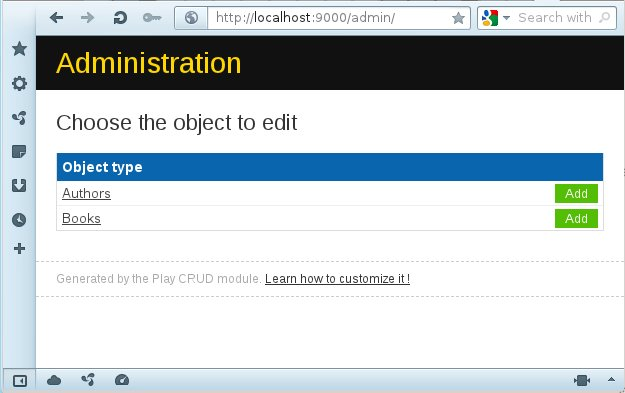
\includegraphics[scale=0.7]{images/crud1.jpeg}}
  \caption[CRUD interface for Play]{Figure depicts the CRUD interface which Play provides for simple model classes.}
  \label{fig:crud1}
\end{figure}
\begin{figure}[p]
  \centering
  \centerline{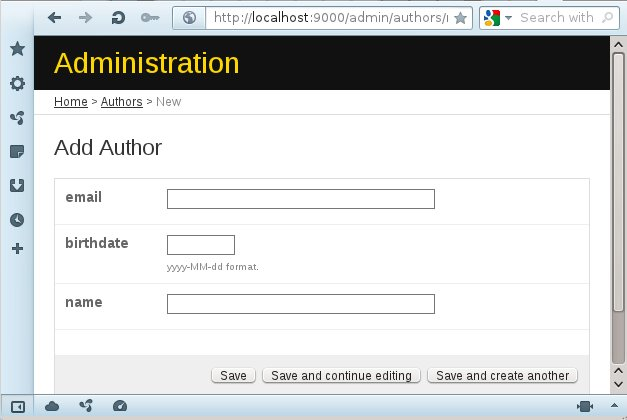
\includegraphics[scale=0.7]{images/crud2.jpeg}}
  \caption[CRUD interface for Play 2]{Figure depicts editing an Author object with the Play CRUD interface.}
  \label{fig:crud2}
\end{figure}

\subsection{Conclusion}
The tutorial has shown how the process of creating a code generator works. We start off by defining our DSML and a sample instance model and corresponding textual output.

Through the chapter we have seen the basic building blocks and features of a Xpand template, everything from defining the output to using extensions for abstracting away complex code. Lastly, we have seen how to generate a simple CRUD interface using Play.

The complete example project can be found at \url{http://dpf.hib.no/downloads/}, which includes Eclipse integration for the project.


% 
% create project in play!
% 
% 
% -constraints er ikkje handheva i generering
% - what to generate -> model classes
%   - input/output slik som definert i kap 3
% -create project
%   - bilete av vegvisar
%   - prosjektstruktur med generert workflow og template
% - defining a template 
%   - constructs som blir brukt
%   - extensions
% - project that uses the generator
% - utfordringar når ein ikkje har symbol, vanskelig å lage oversiktlege diagram.
% - debugging the workflow
% Things to add:
% \begin{itemize}
%     \item Introduction to Play Framework
%     \item How to it works
%     \item Describe process of creating generator from beginning to end
%     \item Illustration showing how the project interacts with *metamodel and *ui
%     \item Illustration showing typed template editor?
% \end{itemize}
\chapter{Conclusion}\label{chap:conclusion}
This chapter will give an overview of what has been achieved through this project. The code generation tool which is developed in this project serves as a proof of concept solution which we will propose further work on. As the thesis has had some focus on the concept of language workbenches, we will propose some further work in this directon as well.

\section{Summary}
Previous efforts to create a DPF based tool has never reached the level of maturity needed to start serious work on code generation. With the work of Øyvind Bech and Dag Viggo Lokøen, we now have a diagrammatic editor which conveys the most important metamodelling concepts in DPF. The editor is built on top of a solid platform that enables us to create rich tooling for the DPF project. Through the chapters of this thesis we have created a solution for metamodel based code generation with the Xpand framework. Like the DPF Editor, this solution is based on Eclipse technologies and is thus well integrated.

Although the creation of a metamodel for Xpand is not a unique concept, we have yet to find any implementations of custom metamodels besides the ones provided with the framework.

Through the project we achieved the following:
\begin{description}
  \item[General solution for creating code generators] \hfill \\
  We have introduced a solution which can be applied to any DSML created with the DPF Editor. The solution provides a functional environment for creating code generators. Creating a metamodel for Xpand has enabled us to use the domain concepts of a DSML when defining templates, extensions and constraints checking. This is possible because the metamodel is a mapping from DPF specifications to types which Xpand understands. We have defined a type system which represents each of the modelling constructs in DPF (i.e. node, arrow, constraint etc.). The types expose the functionality that is defined in the DPF Ecore metamodel, together with additional functionality that is defined to enhance the process of creating code generators.
  \item[Eclipse integration] \hfill \\
  With the implementation of a Xpand metamodel, we get a lot of functionality (almost) for free. Xpand provides a rich editing experience for templates, extensions and constraint checking based on the DPF Xpand metamodel. The editors feature code completion, syntax coloring, refactoring and error highlighting among others.
  \item[Moved DPF Editor towards becoming a language workbench] \hfill \\
  A DSML without any tooling around it is worthless. One of the most essential activities in a language workbench is model transformations, where model-to-text transformations might be the most pragmatic solution. Creating a usable language workbench without the support of creating code is arguably not a language workbench. Although the code generation activity can be seen as separate from creating the language itself, it is indeed part of a language workbench.
\end{description}

\section{Further Work}
This section will propose further work for the code generation tool, as well as some suggestions for features that takes the DPF Editor further towards becoming a language workbench.

\subsection{Code Generation}
The code generation tool should be regarded as a prototype as it have not been properly tested. The following section will explore some of the aspects which can be worked on.

\subsubsection{Work on Shortcomings}
Section~\ref{sec:shortcomings} contains a small list of functionality which is not implemented at the time of writing. The tasks are relatively simple to implement, but might be time consuming.

\begin{description}
  \item[Consistent API:] This is not a shortcoming in the tool itself, but a project-wide problem. When relying on the DPF core API, one is very prone to errors due to modifications in the DPF Ecore metamodel (e.g. changing names, methods etc.). However, the biggest problem with this is rendering all "older" DPF models invalid. A migration strategy is needed, both for the API and models.
  \item[Constraints and predicates as Xpand types:] Predicates and constraints are not properly implemented using their designated types (\codeText{PredicateType} and \codeText{ConstraintType}) for various reasons. The current functionality might be sufficient for now, but hopefully adoption of the tool will help to identify where the need for alterations lies.
  \item[Test coverage:] The DPF Xpand metamodel has not been properly tested. Creating tests is also a challenge, and hard without using DPF models directly. Spending development time on creating model based tests is a waste of time if the models become invalid after the first change to the DPF Ecore metamodel.
  \item[Namespaces:] Implementing the support for more than one DSML per project was not a priority when developing the DPF Xpand metamodel. This is a relatively simple task to achieve.
\end{description}

\subsubsection{Validating Constraints}
The DPF Editor validates the different entities when creating a DSML. Each layer gets checked for the correct typing, and all constraints are validated. When creating a code generator the validation of constraints is left to the user. E.g. if a model has some kind of multiplicity constraint, there is no way to check if the constraint has been fulfilled in the generated code. Xpand provides a constraints checking language called \emph{Check} (see section~\ref{sec:xpand}), but this language works on the Xpand types rather than checking if the template code has fulfilled the constraints, which is defined within the model. Check can however be used to validate the generator's input models if this is desired.

An idea can be to define a post-processor (see Xpand documentation~\cite{xpand}) which scans the output and checks statements against the model.

\subsubsection{Investigate Xtend 2}
In section~\ref{subsec:xtend2}, the Xtend 2 language is introduced as the replacement for Xpand. Xtend 2 is a general programming language (GPL) which compiles to Java. Unfortunately Xtend 2 is not compatible with Xpand as it is a completely different approach (Xpand uses an interpreter). Xtend 2 has not been properly investigated to draw any conclusions on if it can be used in the DPF Editor providing the same functionality as Xpand. At the time of writing there are indications which suggests that Xtend 2 is not able to fulfill the use case that Xpand fills, namely interpreting models runtime, and providing an editing environment based on the content of the model. The good news is that the template language used in Xtend 2 is Xpand, which means any templates written in the current tool, will (largely) be compatible with Xtend 2. This does not apply to any extensions specified, as these are written in Xtend 2.

Although Xpand's future is uncertain, it will be supported a while longer. This means that bugs will be fixed, but no larger releases will occur.

A few solutions to this problem can be:
\begin{itemize}
  \item Migrate our solution to Xtend 2
  \item Fork the Xpand project
  \item Create an in-house code generation solution
  \item Find another solution (e.g. Acceleo)
\end{itemize}
It is the author's opinion (based on the current knowledge) that Xpand is a better solution than Xtend 2. Xtend 2 is a GPL that uses Xpand "template expressions" within the code, thus mixing code and templates. As stated, there does not seem to be any way of interpreting DPF models, which means we are back to using the Ecore instance directly (see section~\ref{sec:problem_description}).

This is not a pressing issue as Xpand is a modern solution with a very stable code base. 

\subsection{Language Workbench}
A part of the DPF project's vision is to create a working tool that increases the developer's productivity, and do not exist solely for academic purposes. This thesis has introduced the term language workbench, which is a pragmatic take on the MDE methodology. In a language workbench the tooling which supports the modeler and its users are of upmost importance. This section will propose further work that will move the DPF Editor even closer towards the goal of becoming a productive language workbench.

\subsubsection{Symbol Editor}
One of the challenges the DPF Editor faces is visualizing the DSMLs. In chapter~\ref{chap:model_based_development} we looked at MetaCase's MetaEdit+ tool, which has the ability to create custom symbols for their \emph{object} modelling entity. This is an effective way of communicating the intent of the language and its concepts. In DPF there is no support for attributes on the nodes, there is only nodes and arrows. A DSML of only nodes and arrows can look a lot more complex than it actually is, which then becomes a usability problem.

To tackle the problem with complex models, one can create create symbols for nodes and arrow. Currently there is support for using simple pre-defined shapes, like ellipse, square, circle etc.

The most recent work by Ph.D. student Xiaoliang Wang has resulted in a signature editor where one can define custom predicates. All predicates needs a symbol, which means a symbol editor would be a nice fit for this requirement as well. The symbol editor can be a simple drawing application, with the possibility of importing graphics.

\subsubsection{Visualization for DSMLs}
Even though symbols will create a better user experience when modelling, the problem of only having nodes and arrows are not dealt with. Our models are centered around graph concepts. A solution to this problem is to create a visualization independent of the underlying model structure. One can group different nodes and arrows, and create a visualization for the group. As an example we could group the \codeText{DomainClass}, \codeText{Attribute} and \codeText{Type} concepts from the DSML in chapter~\ref{chap:case_study}, and create a visualization similar to an UML class.

This way DSML modelers have a greater freedom in how he/she wants to present the domain concepts of the created language. One could also ship the tool with pre-defined DSMLs, visualizations and code generators that defines e.g. UML class diagrams, a language for modelling Android apps, petri-nets etc.

A solution like this is as far as the author knows unique, and would probably give an advantage over other language workbenches.

\subsubsection{Textual Representation of DPF models}
The comparsion at the end of chapter~\ref{chap:model_based_development} mentioned the need for a textual representation of models in addition to projectional representations in language workbenches. Of the more popular solutions on the market, no one seems to have this feature. The language workbenches are either textual or graphical. An optimal solution would be a textual, human readable representation of a DPF model which the graphical representation was based on. Any modifications in either model should be reflected in the other.

We have through Florian Mantz' Ph.D. work, an external DSL for DPF which could be integrated with the DPF Editor.

\subsubsection{File Format}
The current state of file formats in DPF are XMI serializations of the specifications, as well as the corresponding visualization\footnote{The serialization of the visualization is recent work by Ph.D. student Xiaoliang Wang, and was not implemented for the most part of this projects' time span}. A file format could be an archive file which contained all the specifications in a metamodelling hierarchy, together with its visualizations and signature.  If a textual model representation is integrated in the DPF Editor, there needs to be room for this in the file format as well. An important aspect of this task is to create a file handling facility which can keep compatibility between different versions files, and the models within.

\subsubsection{Version Control System for Models}
Creating a VCS for DPF models would be another unique feature for the DPF Editor. This subject was the focus of Alessandro Rossini's Ph.D. thesis~\cite{rossini_thesis_2011} which provides a formal approach to the problem.

\section{Final Words}
The work on this thesis has resulted in a prototype code generation tool, which provide the opportunity to create code generators for an arbitrary DSML. Code generation is an important activity in MDE, and thus an important feature in a language workbench. A usable code generation facility is critical for the success of the DPF Editor.

Even though the Xpand framework's future is uncertain, it is a state of the art tool. The author is confident that Xpand and the prototype developed in this thesis is a solid foundation for further work.
















%%%%%%%%%%%%%%%%%%% APPENDIX %%%%%%%%%%%%%%%%%%%%
%\appendix
%\include{appendix/ap0_eclipsesetup}
%\include{appendix/ap1_resources}

%%%%%%%%%%%%%%%%%%% META CONTENT  %%%%%%%%%%%%%%%%%%%%
% \cleardoublepage
% \phantomsection
% \addcontentsline{toc}{chapter}{List of Figures}
% \listoffigures
% 
\cleardoublepage
\phantomsection
\addcontentsline{toc}{chapter}{Bibliography}
\bibliographystyle{plain}
\bibliography{../bib/bibliography}

%\newpage
%\addcontentsline{toc}{chapter}{Index}
%\printindex

\end{document} 